%%%%%%%%%%%%%%%%%%%%%%%%%%%%%%%%%%%%%%%%%
% Masters/Doctoral Thesis 
% LaTeX Template
% Version 2.5 (27/8/17)
%
% This template was downloaded from:
% http://www.LaTeXTemplates.com
%
% Version 2.x major modifications by:
% Vel (vel@latextemplates.com)
%
% This template is based on a template by:
% Steve Gunn (http://users.ecs.soton.ac.uk/srg/softwaretools/document/templates/)
% Sunil Patel (http://www.sunilpatel.co.uk/thesis-template/)
%
% Template license:
% CC BY-NC-SA 3.0 (http://creativecommons.org/licenses/by-nc-sa/3.0/)
%
%%%%%%%%%%%%%%%%%%%%%%%%%%%%%%%%%%%%%%%%%

%----------------------------------------------------------------------------------------
%	PACKAGES AND OTHER DOCUMENT CONFIGURATIONS
%----------------------------------------------------------------------------------------

\documentclass[
11pt, % The default document font size, options: 10pt, 11pt, 12pt
%oneside, % Two side (alternating margins) for binding by default, uncomment to switch to one side
english, % ngerman for German
singlespacing, % Single line spacing, alternatives: onehalfspacing or doublespacing
%draft, % Uncomment to enable draft mode (no pictures, no links, overfull hboxes indicated)
%nolistspacing, % If the document is onehalfspacing or doublespacing, uncomment this to set spacing in lists to single
%liststotoc, % Uncomment to add the list of figures/tables/etc to the table of contents
%toctotoc, % Uncomment to add the main table of contents to the table of contents
%parskip, % Uncomment to add space between paragraphs
%nohyperref, % Uncomment to not load the hyperref package
headsepline, % Uncomment to get a line under the header
%chapterinoneline, % Uncomment to place the chapter title next to the number on one line
%consistentlayout, % Uncomment to change the layout of the declaration, abstract and acknowledgements pages to match the default layout
]{MastersDoctoralThesis} % The class file specifying the document structure

\usepackage[utf8]{inputenc} % Required for inputting international characters
\usepackage[T1]{fontenc} % Output font encoding for international characters

\usepackage{mathpazo} % Use the Palatino font by default

\usepackage[backend=bibtex,style=authoryear,natbib=true]{biblatex} % Use the bibtex backend with the authoryear citation style (which resembles APA)

\addbibresource{example.bib} % The filename of the bibliography

\usepackage[autostyle=true]{csquotes} % Required to generate language-dependent quotes in the bibliography

% add from other template
\usepackage{amsmath, amssymb}
%\usepackage{graphics} 
\usepackage{wrapfig,lipsum,booktabs}
\usepackage{setspace}
\usepackage{enumerate}
\usepackage{subfigure}
%\usepackage{fancyhdr}
\usepackage{eucal}
\usepackage[below]{placeins}
\usepackage[english]{babel}
%\usepackage[usenames, dvipsnames]{color}
%\usepackage[perpage]{footmisc}
%\usepackage{multirow}
%\usepackage{ifthen}
%\usepackage[square,sort,comma,numbers]{natbib} % Gang
\usepackage{mathrsfs} % Curlicue characters %Gang
%\usepackage{dcolumn}% Align table columns on decimal point %Gang
\usepackage{bm}% bold math %Gang
\usepackage{sidecap} %Gang
% Nomenclature
\usepackage{nomencl}
\usepackage{graphicx} % Include figure files
\usepackage{epstopdf} % PDFLATEX is not able to handle EPS graphic files, but converters epstopdf will help. The best way is to include epstopdf, which must follow the graphicx package
\usepackage{float}  %introduces a placement option H enforcing the placement exactly at that point.
\usepackage{placeins} %provides the command \FloatBarrier to limit the floating of figures or tables. You could place such a barrier before and after a listing.
\usepackage{xcolor}
\usepackage{color}
\usepackage{soul}
\usepackage{xspace} %In order to have space after "\newcommands" 
\usepackage{listings}  %use for listing source codes
%\usepackage[all,cmtip]{xy}  %xypic
\lstset{ 
    language=python, % choose the language of the code
    basicstyle=\fontfamily{pcr}\selectfont\footnotesize\color{black},
    keywordstyle=\color{red}\bfseries, % style for keywords
    numbers=none, % where to put the line-numbers
    numberstyle=\tiny, % the size of the fonts that are used for the line-numbers     
    backgroundcolor=\color{white}, % we can also choose: darkgray
    showspaces=false, % show spaces adding particular underscores
    showstringspaces=false, % underline spaces within strings
    showtabs=false, % show tabs within strings adding particular underscores
    frame=single, % adds a frame around the code
    tabsize=2, % sets default tabsize to 2 spaces
    rulesepcolor=\color{gray},
    rulecolor=\color{black},
    captionpos=b, % sets the caption-position to bottom
    breaklines=true, % sets automatic line breaking
    breakatwhitespace=false, 
}
%\usepackage[toc,page]{appendix} %For adding appendices
\usepackage{pgfplots} % a plotting package in latex
\usepackage[export]{adjustbox}[2011/08/13]

%=================================================
%(Re-)New commands
%=================================================
%\renewcommand{\nomname}{List of Symbols and Abbreviations}
\newcommand{\etal}{\textit{et al.}}
\newcommand{\abinitio}{\textit{ab initio}\xspace}
\newcommand{\Li}{Li$^{+}$\xspace}
\newcommand{\Na}{Na$^{+}$\xspace}
\newcommand{\K}{K$^{+}$\xspace}
\newcommand{\Cl}{Cl$^{-}$\xspace}
\newcommand{\Br}{Br$^{-}$\xspace}
\newcommand{\I}{I$^{-}$\xspace}
\newcommand{\li}{Li$^{+}$}
\newcommand{\na}{Na$^{+}$}
\newcommand{\pot}{K$^{+}$}
\newcommand{\cl}{Cl$^{-}$}
\newcommand{\br}{Br$^{-}$}
\newcommand{\Iodine}{I$^{-}$}
\newcommand{\COO}{COO$^{-}$\xspace}
\newcommand{\sfg}{Sum Frequency Generation\xspace}
\newcommand{\cm}{cm$^{-1}$~\xspace}
\newcommand{\centimeter}{cm$^{-1}$}
\newcommand{\nm}{nm$^{-2}$\xspace}
\newcommand{\z}{\textit{z}-axis\xspace}
\newcommand{\water}{H$_2$O\xspace}
\newcommand{\wat}{H$_2$O}
\newcommand{\NVT}{\textit{NVT}\xspace}
\newcommand{\T}{\textit{T}\xspace}
\newcommand{\nitrate}{NO$_3^-$\xspace}
\newcommand{\nit}{NO$_3^-$}
\newcommand{\LiN}{LiNO$_3$\xspace}
\newcommand{\X}{$x$\xspace}
\newcommand{\Y}{$y$\xspace}
\newcommand{\Z}{$z$\xspace}

%
\newcommand{\CHB}{$C_{\text{HB}}(t)$\xspace}
\newcommand{\SHB}{$S_{\text{HB}}(t)$\xspace}

%Renew the \AA command in order to have a space when we want
\let\oldAA\AA
\renewcommand{\AA}{\oldAA\xspace}
\newcommand{\A}{\oldAA}
%=================================================

%----------------------------------------------------------------------------------------
%	MARGIN SETTINGS
%----------------------------------------------------------------------------------------

\geometry{
	paper=a4paper, % Change to letterpaper for US letter
	inner=2.5cm, % Inner margin
	outer=3.8cm, % Outer margin
	bindingoffset=.5cm, % Binding offset
	top=1.5cm, % Top margin
	bottom=1.5cm, % Bottom margin
	%showframe, % Uncomment to show how the type block is set on the page
}

%----------------------------------------------------------------------------------------
%	THESIS INFORMATION
%----------------------------------------------------------------------------------------

\thesistitle{Structure, Dynamics and Vibrational Spectroscopy of Interfacial 
Alkali Nitrate Aqueous Solutions from \abinitio Molecular Dynamics} % Your thesis title, this is used in the title and abstract, print it elsewhere with \ttitle
\supervisor{Apl. Prof. Dr. Marialore \textsc{Sulpizi}} % Your supervisor's name, this is used in the title page, print it elsewhere with \supname
\examiner{} % Your examiner's name, this is not currently used anywhere in the template, print it elsewhere with \examname
\degree{Doctor of Philosophy} % Your degree name, this is used in the title page and abstract, print it elsewhere with \degreename
\author{Gang \textsc{Huang}} % Your name, this is used in the title page and abstract, print it elsewhere with \authorname
\addresses{} % Your address, this is not currently used anywhere in the template, print it elsewhere with \addressname

\subject{Statistical Physics and Soft Matter} % Your subject area, this is not currently used anywhere in the template, print it elsewhere with \subjectname
\keywords{sum-frequency generation, hydrogen bond dynamics, water/vapor interfaces} % Keywords for your thesis, this is not currently used anywhere in the template, print it elsewhere with \keywordnames
\university{\href{https://www.uni-mainz.de}{Johannes Gutenberg Universit\"at Mainz}} % Your university's name and URL, this is used in the title page and abstract, print it elsewhere with \univname
\department{\href{https://www.iph.uni-mainz.de}{Institute for Physics }} % Your department's name and URL, this is used in the title page and abstract, print it elsewhere with \deptname
\group{\href{https://www.komet1.physik.uni-mainz.de}{Condensed Matter Theory Group}} % Your research group's name and URL, this is used in the title page, print it elsewhere with \groupname
\faculty{\href{https://www.komet1.physik.uni-mainz.de}{Condensed Matter Theory}} % Your faculty's name and URL, this is used in the title page and abstract, print it elsewhere with \facname

\AtBeginDocument{
\hypersetup{pdftitle=\ttitle} % Set the PDF's title to your title
\hypersetup{pdfauthor=\authorname} % Set the PDF's author to your name
\hypersetup{pdfkeywords=\keywordnames} % Set the PDF's keywords to your keywords
}

\begin{document}

\frontmatter % Use roman page numbering style (i, ii, iii, iv...) for the pre-content pages

\pagestyle{plain} % Default to the plain heading style until the thesis style is called for the body content

%----------------------------------------------------------------------------------------
%	TITLE PAGE
%----------------------------------------------------------------------------------------

\begin{titlepage}
\begin{center}

\vspace*{.06\textheight}
{\scshape\LARGE \univname\par}\vspace{1.5cm} % University name
\textsc{\Large Doctoral Thesis}\\[0.5cm] % Thesis type

\HRule \\[0.4cm] % Horizontal line
{\huge \bfseries \ttitle\par}\vspace{0.4cm} % Thesis title
\HRule \\[1.5cm] % Horizontal line
 
\begin{minipage}[t]{0.4\textwidth}
\begin{flushleft} \large
\emph{Author:}\\
\href{http://www.johnsmith.com}{\authorname} % Author name - remove the \href bracket to remove the link
\end{flushleft}
\end{minipage}
\begin{minipage}[t]{0.4\textwidth}
\begin{flushright} \large
\emph{Supervisor:} \\
\href{https://www.staff.uni-mainz.de/sulpizi}{\supname} % Supervisor name - remove the \href bracket to remove the link  
\end{flushright}
\end{minipage}\\[3cm]
 
\vfill

\large \textit{A thesis submitted in fulfillment of the requirements\\ for the degree of \degreename}\\[0.3cm] % University requirement text
\textit{in the}\\[0.4cm]
\groupname\\\deptname\\[2cm] % Research group name and department name
 
\vfill

{\large \today}\\[4cm] % Date
%\includegraphics{Logo} % University/department logo - uncomment to place it
 
\vfill
\end{center}
\end{titlepage}

%----------------------------------------------------------------------------------------
%	DECLARATION PAGE
%----------------------------------------------------------------------------------------

\begin{declaration}
\addchaptertocentry{\authorshipname} % Add the declaration to the table of contents
\noindent I, \authorname, declare that this thesis titled, \enquote{\ttitle} and the work presented in it are my own. I confirm that:

\begin{itemize} 
\item This work was done wholly or mainly while in candidature for a research degree at this University.
\item Where any part of this thesis has previously been submitted for a degree or any other qualification at this University or any other institution, this has been clearly stated.
\item Where I have consulted the published work of others, this is always clearly attributed.
\item Where I have quoted from the work of others, the source is always given. With the exception of such quotations, this thesis is entirely my own work.
\item I have acknowledged all main sources of help.
\item Where the thesis is based on work done by myself jointly with others, I have made clear exactly what was done by others and what I have contributed myself.\\
\end{itemize}
 
\noindent Signed:\\
\rule[0.5em]{25em}{0.5pt} % This prints a line for the signature
 
\noindent Date:\\
\rule[0.5em]{25em}{0.5pt} % This prints a line to write the date
\end{declaration}

\cleardoublepage

%----------------------------------------------------------------------------------------
%	QUOTATION PAGE
%----------------------------------------------------------------------------------------

\vspace*{0.2\textheight}

\noindent\enquote{\itshape The accurate description of water has been and continues to be a challenge for both
experiment and simulations due to the directional nature and the weakness of the hydrogen bonds in conjunction 
with its autodissociation properties.}\bigbreak

\hfill Dominik Marx  and J\"urg Hutter 

%----------------------------------------------------------------------------------------
%	ABSTRACT PAGE
%----------------------------------------------------------------------------------------

\begin{abstract}
\addchaptertocentry{\abstractname} % Add the abstract to the table of contents
I have analyzed the interfacial structure and dynamics of solutions containing alkali nitrates by Density Functional Theory-based 
Molecular Dynamics (DFTMD) simulations. In particular I have presented a detailed analysis of the Hydrogen Bond (HB) structure at the interface and 
have calculated the interface vibrational spectra in order to provide a molecular interpretation of available experimental data.
%
As a first system I have analyzed the behaviour of a salty water/vapor interface containing LiNO$_3$.
Both the measured and calculated Vibrational Sum-Frequency Generation (VSFG) spectra shows a reduced intensity of the lower frequency portion region,
when compared to the pure water/vapor interface.
This reduction is attributed to the H-bonds established between the \nitrate and the surrounding water molecules at the interface.
This effects is only related to the presence of \nitrate at the water surface and is not affected by the presence of alkali metal ions.
I have shown that although the \Li can reside relative close to the water surface, also forming a water mediated
ion pair with \nit, its effect on the VSFG spectrum is not visible. The water molecule which mediate the interaction
between the \nitrate and the \Li would produce a red-shifted peak in small water cluster, but its influence is not visible
neither in the VSFG spectra.
I have shown that the use of simple models, such as small cluster is not suitable to reproduce the experimental spectra 
and cannot provide a microscopic interpretation of the spectra.
Realistic models of the interface are required to address the perturbation of the ion on the water surface.
%
The difference between the HB dynamics outside the first shell of the \Li and that of nitrate-water Hydrogen (H-) bonds
at interfaces is not visible from the values of the HB relaxation time. They reflect the difference 
between HB dynamics in bulk water and that at the water/vapor interfaces.
For the water/vapor interface of alkaline iodine solutions, I find that the cations does not alter the H-bonding network outside the first hydration shell of cations.
It is concluded that no long-range structural-changing effects for alkali metal cations.
%
From the results of nonlinear susceptibilities, I conclude that these water molecules at the water/vapor interfaces of LiI, NaI, and KI solutions are participating
in weaker H-bonds, compared with those at the pure water surface.
The origin of the characteristics may come from a unique distribution of \I ions and alkali metal cations,
which form a double layer over the thickness on the order of 5--10 \A.
%
Finally, I obtain that faster rotational anisotropy decay exists for water molecules at the interface of aqueous alkali-iodine solutions, 
which is the result of a different HB types from the usual HB type in pure bulk water. 
This effect on anisotropy decay is due to the H--I bond at the interface.
This difference of HB structure from pure water/vapor interface changed the Im$\chi^{(2),\text{R}}$ spectrum
and the HB dynamics of the interface of alkali-iodine solution.
\end{abstract}

%----------------------------------------------------------------------------------------
%	ACKNOWLEDGEMENTS
%----------------------------------------------------------------------------------------

\begin{acknowledgements}
\addchaptertocentry{\acknowledgementname} % Add the acknowledgements to the table of contents
I wish to express my sincere gratitude to my supervisor,
Prof. Dr. Marilore Sulpizi for her excellent guidance during my research, and her detailed and valuable advice for my writing.
I thank her for bringing me into interesting and novel areas of density functional theory-based molecular dynamics simulation 
and interface physics and chemistry. By communicating with her, I was implicitly and positively affected. 
She is rigorous in academic studies, optimistic and active, and has a wide range of interests. 
All these have kept in my heart and gave me greater confidence in future scientific research work.

I wish to thank Prof. Dr. Thomas Kühner, Dr. Giovanni Settanni, Dr. Peter
Virnau, Dr. Hans Behringer, Prof. Dr. Thomas Speck and in the Institute for
Physics for leading me to the fundamental statistical physics and excellent lectures
and discussions. I am grateful to Prof. Dr. Friederike Schmid and Prof. Dr. Kurt
Binder for their talks and guidance.

I am grateful to Dr. R\'emi Khatib for programing skills and helpful guidance on
the programs for calculating the VSFG spectra. I also thank Dr. Shuanhu Qi, Dr. Jiajia Zhou and Dr. Fei Yu for useful discussions 
on the the calculation of response functions. I would like to
thank my colleagues Leila Salimi, Isidro Lorenzo Geada, Santosh Kumar Meena and Anusha Lalitha, 
at the Institute for Physics, for their encouragement and assistance.

I am grateful to my parents Dehuai Huang and Yuhua Diao and my brother Jialiang Huang for being there for me during the
last years.

The financial supports of the China Scholarship Council and TRR146 are gratefully acknowledged.
\end{acknowledgements}

%----------------------------------------------------------------------------------------
%	LIST OF CONTENTS/FIGURES/TABLES PAGES
%----------------------------------------------------------------------------------------

\tableofcontents % Prints the main table of contents

\listoffigures % Prints the list of figures

\listoftables % Prints the list of tables

%----------------------------------------------------------------------------------------
%	ABBREVIATIONS
%----------------------------------------------------------------------------------------

\begin{abbreviations}{ll} % Include a list of abbreviations (a table of two columns)

\textbf{ACF} & \textbf{A}uto-\textbf{C}orrelation \textbf{F}unction\\
\textbf{AIMD} & \abinitio \textbf{M}olecular \textbf{D}ynamics\\
\textbf{BLYP} & \textbf{B}eck-\textbf{L}ee-\textbf{Y}ang-\textbf{P}arr\\
\textbf{BOMD} & \textbf{B}orn-\textbf{O}ppenheimer \textbf{M}olecular \textbf{D}ynamics\\
\textbf{CPMD} & \textbf{C}ar-\textbf{P}arrinello \textbf{M}olecular \textbf{D}ynamics\\
\textbf{DFT} & \textbf{D}ensity \textbf{F}unctional \textbf{T}heory\\
\textbf{DFTMD} & \textbf{D}ensity \textbf{F}unctional \textbf{T}heory-based \textbf{M}olecular \textbf{D}ynamics\\
\textbf{GGA} & \textbf{G}eneralised \textbf{G}radient \textbf{A}pproximation\\
\textbf{HB} & \textbf{H}ydrogen \textbf{B}ond\\
\textbf{HK} & \textbf{H}ohenberg-\textbf{K}ohn\\
\textbf{KS} & \textbf{K}ohn-\textbf{S}ham\\
\textbf{LDA} & \textbf{L}ocal \textbf{D}ensity \textbf{A}pproximation\\
\textbf{MD} & \textbf{M}olecular \textbf{D}ynamics\\
\textbf{MP2} & \textbf{M}oller-\textbf{P}lesset \textbf{P}erturbation\\
\textbf{PBE} & \textbf{P}erdew-\textbf{B}urke-\textbf{E}rnzherhof\\
\textbf{PS} & \textbf{P}hase-\textbf{S}ensitive\\
\textbf{RDF} & \textbf{R}adial \textbf{D}istribution \textbf{F}unction\\
\textbf{SCF} & \textbf{S}elf \textbf{C}onsistent \textbf{F}ield\\
\textbf{VDOS} & \textbf{V}ibrational \textbf{D}ensity \textbf{O}f \textbf{S}tates\\
\textbf{VSFG} & \textbf{V}ibrational \textbf{S}um-\textbf{F}requency \textbf{G}eneration\\
\textbf{XC} & e\textbf{X}change  and \textbf{C}orrelation\\

\end{abbreviations}

%----------------------------------------------------------------------------------------
%	PHYSICAL CONSTANTS/OTHER DEFINITIONS
%----------------------------------------------------------------------------------------

\begin{constants}{lr@{${}={}$}l} % The list of physical constants is a three column table

% The \SI{}{} command is provided by the siunitx package, see its documentation for instructions on how to use it

speed of light in vacuum  & $c$ & \SI{299 792 458}{\meter\per\second} (exact)\\
%Constant Name & $Symbol$ & $Constant Value$ with units\\
Boltzmann constant & $k_{\text{B}}$ & 1.380 650 3(24)$\times 10^{23}$ \si{\joule\per\kelvin} \\
elementary charge & $e$  & 1.602 176 462(63)$\times 10^{-19}$ C \\
electron mass & $m_{\text{e}}$ & 9.109 381 88(72) $\times 10^{-31}$ kg \\
proton mass & $m_{\text{p}}$ & 1.672 621 58(13) $\times 10^{-27}$ kg \\
Avogadro constant & $N_{\text{A}}$ & 6.022 141 99(47) $\times 10^{23}$ mol \\
Planck constant & $h$ & 6.626 068 76(52) $\times 10^{-34}$ J s \\
molar gas constant & $R$ & 8.314 472(15) J mol$^{-1}$ K$^{-1}$
\end{constants}

%----------------------------------------------------------------------------------------
%	SYMBOLS
%----------------------------------------------------------------------------------------

\begin{symbols}{lll} % Include a list of Symbols (a three column table)

% $a$ & distance & \si{\meter} \\
% $P$ & power & \si{\watt} (\si{\joule\per\second}) \\
% $\omega$ & angular frequency & \si{\radian} \\
%Symbol & Name & Unit \\

\addlinespace % Gap to separate the Roman symbols from the Greek

$Z_{\text{X}}$ & atomic number of atom X & \\
$\tau_{\text{HB}}$ & average lifetime of H-bonds & \\
$\kappa_i$ & decay rate of $C_2(t)$ & \\
$n_{\text{X}}$ & coordination number of ion X & \\
${\bf M}$ & dipole moment & \\
$\mu^{i,l,\epsilon}$ & dipole moment of the bond $\epsilon$ of the $i$-th water molecule in the lab frame & \\
$A$ & dipole polarizability (tensor) & \\
$D$ & direction cosine matrix  & \\
$r$ & distance & \\
${\mu}$ & electric dipole vector & \\
${\bf E}$ & electric field strength &  \\
$V_{\text{ee}}$ & electron-electron repulsion energy & \\
$E_{\text{disp}}^{(2)}$ & empirical two-body dispersion correction of energy & \\
$E_{\text{disp}}^{(3)}$ & empirical three-body nonadditivity dispersion correction of energy & \\
$\Delta F_{AB}$ & free energy difference between configuration A and B &  \\
$F_A$ & free energy of configuration A &  \\
$L_{\eta\kappa}$ & Fresnel coefficients & \\
$\omega_{\text{SFG}}$ & frequency of the sum-frequency generation beam & \\
$\omega_{\text{vis}}$ & frequency of the incident visible beam &  \\
$\omega_{\text{IR}}$ & frequency of the incident infrared beam &  \\
$h(t), H(t)$ & HB population operators & \\
$C_{\text{HB}}$ & HB population operator correlation function & \\
$\omega_{\text{I}}$ & highest nuclear phonon frequency & \\
$\theta$ & H-O-H angle in a water molecule&  \\
$\beta$ & hyperpolarizability; reciprocal temperature & \\
$j(t)$ & integrated flux departing the HB configuration space at time t & \\
$I_{\text{SFG}}$ & intensity of the sum-frequency generation beam & \\
$I_{\text{vis}}$ & intensity of the incident visible beam & \\
$I_{\text{IR}}$ & intensity of the incident infrared beam & \\
$r_{\text{OO}}$ & interoxygen distance & \\
$\omega_{\text{e}}$ & the lowest electronic frequency &  \\
$r_{\text{OO}}^{\text{c}}$ & the maximum value of the interoxygen distance in the definition of HB & \\
$\phi^{\text{c}}$ & the maximum value of the angle between the O--O axis and one of the O--H bonds in the &  \\
                  & definition of HB & \\
$N$ & number of water molecules & \\
$R_{\text{OH}}$ & O-H length in water molecule & \\
$C_2(t)$ & orientational anisotropy decay & \\
$Z$ & partition function & \\
$\alpha$ & polarizability tensor & \\
$\alpha^{i,l,\epsilon}$ & polarizability of the bond $\epsilon$ of the $i$-th water molecule in the lab frame & \\
$P(t)$ & probability distribution of HB lifetime & \\
$C_z(t)$ & projected velocity auto-correlation function along $z$-axis & \\
$x^{\text{l}},y^{\text{l}},z^{\text{l}}$ & position coordinates in the lab frame  & \\
$x^{\text{m}},y^{\text{m}},z^{\text{m}}$ & position coordinates in the molecular frame  & \\
$x^{\text{b}},y^{\text{b}},z^{\text{b}}$ & position coordinates in the bond frame  & \\
$g_z(\nu)$ & projected VDOS for selected atoms along $z$-axis &  \\
$g_{\text{A--B}}$ & radial distribution function & \\
$k$ & rate constant of breaking an HB & \\
$\theta_{\text{SFG}}$ & reflected angle of SFG beam with respect to the normal direction in the medium  & \\ 
$k(t)$ & reactive flux & \\
$\tau_{\text{R}}$ & relaxation time of HB population operator correlation function & \\
$P_2(x)$ & the second Legendre polynomial &  \\
$\chi^{(2),\text{R}}$ & second-order resonant susceptibility & \\
$\chi^{(2),\text{NR}}$ & second-order nonresonant susceptibility & \\
$E_{\text{KSDFT}}$ & self consistent KS energy & \\
$\Delta \nu'$  & shift of vibrational frequency & \\
$K_{\text{p,X}}$ & surface/bulk molar concentration ratio of ion X &  \\
$S_{\text{HB}}$ & survival probability of HB & \\
$t_t$ & temporal resolutions for calculating HB dynamics & \\
$d$ & thickness of layer of interface (model) & \\
$\hat{\mu}(t)$ & unit vector of the transition dipole & \\
$g(\nu)$ & VDOS for selected atoms &  \\
${\bf v}$ & velocity of an atom & \\
$C(t)$ & velocity auto-correlation function & \\
$\nu$ & vibrational frequency & \\
\end{symbols}

%----------------------------------------------------------------------------------------
%	DEDICATION
%----------------------------------------------------------------------------------------

\dedicatory{To my parents Dehuai Huang and Yuhua Diao, and my brother Jack Huang.} 

%----------------------------------------------------------------------------------------
%	THESIS CONTENT - CHAPTERS
%----------------------------------------------------------------------------------------

\mainmatter % Begin numeric (1,2,3...) page numbering

\pagestyle{thesis} % Return the page headers back to the "thesis" style

% Include the chapters of the thesis as separate files from the Chapters folder
% Uncomment the lines as you write the chapters

\chapter{Introduction}\label{CHAPETR_1}
%Why ions at water/vpaor important?
%Water and aqueous solution are indispensable to life.
Interfaces of water and electrolyte solutions exist in many biological and industrial chemical systems, and
are essential for all kinds of physical [\cite{Yamamoto2008, Salmeron2009,Balajka2018}] and chemical processes. [\cite{Tobias99,Benderskii00,Benderskii02}]
Many phenomena in biology and chemistry, such as adsorption,
bubble formation, occur at aqueous interfaces. [\cite{Ball2008}]
Particularly, water/vapor interfaces are the most common liquid interface. [\cite{Kuo2004b}] 
Water/vapor interfaces of aqueous solutions play a important role in environmental chemistry, biological systems, [\cite{ZhangLY09,Nostro12}] 
man-made systems [\cite{Richmond02,LiuH04,Asahi01}] and atmospheric science. [\cite{TianCS08,Irwin88}] 
%2.
Ions at the water/vapor interface can undergo heterogeneous or interfacial reactions. [\cite{HuJH95,LiuDF04,Clifford07,Manna13,Pillar2014}] 
%for example, water accelerate organic reactions under heterogeneous condition.\cite{Manna13} 
%Heterogeneous reactions of ozone with bromide at the water/vapor interface of NaBr aerosol were observed, 
%by Clifford and Donaldson, with measuring pH changes associated with the interfacial reaction of ozone and bromide\cite{Clifford07}.
%In 2014, Pillar et.al.'s work shows a scheme that catechol, a molecular probe of the oxygenated aromatic hydrocarbons, 
%present in secondary organic aerosols, contribute interfacial reactive species, which enhance the production 
%of humic-like substances under atmospheric conditions.\cite{Pillar2014} It also implys that catechol undergoes fast oxidation 
%at the water/vapor interface by some competing pathways.
%Reactions between gases and halide anions are enhanced at the interfaces.\cite{HuJH95,LiuDF04}
%3.
Therefore, the distribution of ions at water/vapor interfaces is essential for understanding the structure and dynamics of interfaces. 
The hydrogen (H-) bonding network \cite{Einsenberg1969,Speedy1976,Poole1992,Soper2008,Nilsson2011,Ball2001,Pettersson2015} as well as electrostatic force, and van der Waals force are the main factors that determine the structure of interfaces. 
Salts change the H-bonding structure of water in the interfacial region. [\cite{EAR04,McLain2006,Ball2008}] 
The difference between anions' distribution may have significant influence on the H-bonding network of interfacial water. [\cite{Morita2008}]

%Fact: 
Compared to bulk atoms or molecules,
interfacial atomic or molecular layers generally have very different optical properties. 
Experimentally, in order to determine the structure of an interface, one can use Vibrational Sum-Frequency Generation (VSFG) spectroscopy.
%What VSFG can provide for water/vapor interface?
The VSFG spectroscopy utilizes a second-order nonlinear optical process and the resulting signal is very sensitive to surface ions and 
molecules of a submonolayer level. [\cite{Morita2008,WangHongFei2015,WenYuChieh2016,Ishiyama2017,Penalber-Johnstone2018}] 
This technique allows for detecting intramolecular vibrational modes, and molecular orientation by detecting polarization dependence of the VSFG signals. [\cite{Vidal05}]  
Furthermore, the VSFG spectroscopy does not require ultrahigh-vacuum environment. [\cite{WeiX02}]
The advantage is its wide applicability to almost every interface as long as light can reach them. 
Therefore, the VSFG spectroscopy can be used to probe many types of interfaces, namely, liquid-liquid and 
solid-liquid interfaces. [\cite{Guyot-Sionnest1987,RS91,Du93,QD94,Richmond02,Gopalakrishnan2006,ShenYR2006,Morita2008}]
With the electric dipole approximation, the VSFG process is forbidden in any centrosymmetric bulk medium, [\cite{Che12}] 
such as isotropic liquids and glasses,  but it is allowed at interfaces because of the broken inversion symmetry at the interfaces. [\cite{PF00}]
%DONE from vsfg spectra?
The VSFG spectroscopy can also be applied to metal and semiconductor surfaces. [\cite{Harris87,Superfine88}]
The VSFG spectra suggest that the interfacial H-bonding between water molecules is changed by the presence of salt, 
especially the anions. [\cite{EAR04}]
%The progress of theoretical support for the VSFG spectra?
Molecular-level properties of interfacial materials arising from interactions between water and minerals, 
such as swelling, wetting, hydrodynamics can also be studied by the VSFG spectroscopy. [\cite{Rotenberg14}]

%There are still two problems in VSFG spectra.
However, the quantitative interpretation of the VSFG spectra is not straightforward,
because the VSFG intensity is influenced by several factors, including ions' concentration, 
molecular orientation and distribution and local field correction. \cite{Morita2008}

%[Known]
%Progress of the study of interfacial structure (a)
Although there is some general consensus on the fact that anions propensity inversely correlates with
the order of the Hofmeister series, namely 
CO$_3^{2-}$ $>$  SO$_4^{2-}$ $>$ F$^-$ $>$ Cl$^-$ $>$ Br$^-$ $>$ NO$_3^-$ $>$ I$^-$ $>$ ClO$_4^-$ $>$ SCN$^-$, [\cite{PJ06,ZYJ10,DT08,DFP11}]
the driving force and the microscopic details of the solvation structure are still debated. 
%[DONE for water/vapor interface--Simulations] 
%Progress of the study of interfacial structure (b)
In terms of the Gibbs adsorption equation, the traditional theory predicts that 
no atomic ions will exist at interfacial regions of solutions. However, 
Molecular Dynamics (MD) simulations have shown that more polarizable anions (e.g., larger halide anions) are present in the surface region. [\cite{PJ01,PJ02}] 
Tian and coworkers [\cite{CST11}] also have predicted that some ions, such as \I and Br$^{-}$, could accumulate at the interface.
%Auer and Skinner\cite{Auer08} found that water molecules, at the water/vapor interface, without an H-bond to the H atom are responsible for the distinct shoulder on the blue side of the Raman spectra, by decomposing the transition frequency distribution into subdistributions for water molecules in different H-bonding environments.
%Caleman and coworkers tried to interprete halide ions' surface preference by molecular simulations of alkali and halide ions in water droplets, 
%by using physical properties of ions, such as water-water interaction, ion-water energy, entropy and polaribability, without using chemical properties.\cite{Caleman11}
%Done for infering properties of water/vapor interface
The surface tension has been used to infer the composition of water/vapor interface, 
since the surface tension of the water/vapor interface is generally altered by dissolved substance. [\cite{PJ02}]

%[The ions propensity for the water/vapor interface, as well as their influence on  
%the water's hydrogen bond (HB) network are of special interest to the atmospheric chemistry 
%community.\cite{FPBJ,BJ} Various ions play critical roles in the kinetics 
%and mechanisms of heterogeneous chemical reactions at the water/vapor interface of atmospheric aerosols. 
%The use of surface specific vibrational spectroscopy techniques has 
%permitted to elucidate some aspects of surface HB structure for water in 
%the presence of ions.\cite{AJ12,AGL05} The influence of molecular ions such as nitrate­, sulfate­ and 
%carbonate ions­ has also been analyzed, but proved more elusive than that for halide solution. \cite{SG05,PS03}
%Recently lots of attention has been driven by the nitrate ions in aqueous phase for their 
%ubiquitous role in atmospheric aerosols from polluted water to the remote troposphere.
%\cite{BJ}]

%How to calculate VSFG spectra?
%Unlike an absorption spectrum, the Vibrational Sum-Frequency Generation (VSFG) signal can be considered as a sum of signed contributions 
%from different hydrogen-bonded species in the sample.\cite{Pieniazek11}
%[Done]O: 
%Pieniazek and coworkers\cite{Pieniazek11} had shown that the observed positive feature at low frequency, in the imaginary part of
%the VSFG signal, is a result of cancellation between the positive contributions from four-hydrogen-bonded
%molecules and negative contributions from those molecules with one or two broken H-bonds.

%Via the Gibbs adsorption equation, it has been known that, in 
%aqueous solutions of simple inorganic salts, such as the
%alkali halides, the surface tension increases with solute concentration.\cite{PJ01}
%Traditional thermodynamic model suggests ions in water should be
%repelled from the water/vapor interface, but recent 
%MD simulations have predicted that some ions, such as
%\I and Br$^{-}$, could accumulate at the interface.\cite{CST11,PJ01}

% 5th
%[REMOVE] 
%[Progress of the study of HB dynamics of the interface (a)]
% Second, H-bonding network is important for interfaces of aqueous electrolyte solutions.
%The microscopic structure of water is determined by O-H$\cdots$O H-bonds between the hydroxy group 
%and O atoms of neighboring molecules. Therefore, the H-bonded network of water molecules determines complex structural changes 
%and properties on ultrafast time scales.\cite{Stenger01, Jimenez94,SC02}
%Processes such as aqueous solvation and the transport of protons is governed by liquid water's properties, 
%and these properties arise from the motions of water molecules within a constantly changing H-bonding network.\cite{CJF03}
%Because of the H-bonding, electrostatic force and dispersion forces, 
%at water/vapor interfaces there exists an interface-specific bonding network, 
%which is different from H-bonding network in corresponding bulk liquid.\cite{Allongue96,Velasco-Velez14}
%The structural relaxation of the protein also arise from the relaxation of the H-bonding network 
%via solvent translational displacement.\cite{Tarek02} In experimental situations, the presence of ions in aqueous 
%electrolyte solutions may significantly change the property of the H-bonding network. 
%The formation of H-bonding network indicates a reduction in the orientational degree of freedom, 
%an enhancement in the local structure of water around the solute, or change (decrese) of entropy.\cite{Frank45a, Frank45b,Frank45c}
%The iceberg model was proposed to consider the anomalously large decrease in entropy during hydration.\cite{Frank45c}

%DONE for HBD
%The femtosecond InfraRed Spectroscopy (fsIRS) has been used as a new experimental tool to see the HB dynamics in ionic hydration shells.\cite{Laage07} 
%Tominaga and coworkers studied the dynamical structure of water in the presence of alkali-metal and halide ions as functions of temperature and concentration, 
%by using the low frequency Raman spectroscopy. 
%They found that the water-water intermolecular stretching frequency decrease with increasing ion concentration.\cite{KM98,Amo00}

%H-Bonds act as bridges between protein binding sites and their substrates. \cite{Ball05}
%The structure and dynamics of H bonds play an important role in determining the thermodynamic properties of biomolecules in aqueous solutions.\cite{HX01}  Water’s HB dynamics is also intimately connected to its ultrafast vibrational dynamics.\cite{Nagata15} The dynamic process of rupturing and reforming of H-bonds is water solution can be indirectly probed by a number of experimental methods.\cite{OC84,JT85}  The dynamical response of water is intimately related to the lifetime of H-bonds.\cite{SP05}) Although it can not be yield by experimental methods, it can be studied by computer simulations.\cite{DCR83,VPV09}
%Computer simulations are tools for the study of  hydrogen-bond kinetics near the solvated ions and biomolecules. \cite{PJR79,YKC98}
%Reactive halogen atoms involved in catalytic reactions are main resource to the Arctic tropospheric ozone depletion. \cite{Foster97,Knipping00,Oum98} 

% WE HAD KNOW THE PROBLEM, THEN HOW TO SET UP OUR MODELS and START TO TRYING TO SOLVE THEM
%The structural and dynamical properties of aqueous solutions have been long studied, but the basic physical
%property has not been fully clarified.
%Complex ions, such as nitrate (\nitrate) and ammonium (NH$_4^+$) ions,
%are abundant in environmental and  atmospheric chemistry.\cite{SG05,Yadav2017} 
%Nitrate ions containing in water affect the properties of water, and therefore human beings as well.\cite{Comly45,Knobeloch00} 
%Raymond and Richamond have shown that there exists anions in the surface region of aqueous solutions of alkali halide salts, 
%by using VSFG spectroscopy and comparing the VSFG signal from four alkali halide salt solutions---NaF, NaCl, NaBr 
%and NaI. 
Recently considerable attention has been given to the nitrate ions in aqueous phase 
for their ubiquitous and diverse role in atmospheric aerosols, polluted water, 
and the remote troposphere. [\cite{XuM2009,Jubb2012}]
In order to clarify the variations of the structural and dynamical properties 
of water containing ions with high surface propensity, MD simulations are a valuable tool, 
which can provide detailed information on the structure and dynamics  
of water in a simple and well-known system like alkali metal nitrate and alkali metal halide solutions. [\cite{KM98}]
%Lots of researchers have studied the dynamical structure of aqueous solutions by using low-frequency Raman spectroscopy (LF-RS).\cite{Ujike99} 
%A femtosecond laser technique enables one to investigate the dynamical property of water by Raman induced Kerr effect
%spectroscopy (RIKES).\cite{Mizoguchi92,Righini93}
%
%Useful models for investigating HB dynamics includes the Jump model, extended jump model\cite{Laage07};
%The analytic kinetic model connected to $C(t)$;\cite{Laage07}
%monoexponential decay, characterized by the reorientation time $\tau_2$, of the orientational time correltion function:
%$C(t)=\langle P_2[{\bf u}(0)\cdot{\bf u}(t)]$, where $P_2$ is the second-rank Legendre polynomial and ${\bf u}$ is the OH-bond direction vector.
%Chloride diffusion constant in water, is calculated from simulations through the ion mean-square displacement 
%$D=\lim\limits_{t\to\infty} 1/6t \langle |r(t)-r(0)|^2\rangle$\cite{Laage07}.
%
%DONE by others
In recent years, MD simulations have been used for calculating properties, 
such as the depth profile of ion concentrations of interfaces, [\cite{PJ01,PJ02}]
and the VSFG spectra of electrolyte solution surfaces, [\cite{Gopalakrishnan2006,Johnson2014,Ishiyama2014,Ishiyama2017}] 
but the results depend heavily on the molecular model and interaction potentials used. [\cite{LXD03,MKP04,TI07,MM05}]
In this thesis, we use Density Functional Theory-based Molecular Dynamics (DFTMD) simulations to compute 
the interfacial VSFG spectra of eletrolyte solutions and to provide their molecular interpretation.
The advantageof DFTMD is that it does not require a priori parameterization and it is capable to include polarization effects, [\cite{Ufimtsev2011}]
also including electronic polarization. DFTMD at the gradient corrected level, and also including dispersion corrections [\cite{Grimme04,Grimme06,Grimme07,Grimme10,Baer2011}] 
has been shown to provide an accurate description of the vibrational properties at interface. [\cite{Fornaro2015}]
%[anisotropy dynamics is important] 
%In bulk water, measuring the anisotropy dynamics of O-H stretch vibrations\cite{Woutersen99} demonstrated the rapid F{\"o}rster resonant energy transfer between O-H vibrations of different water mmolecules.

%This thesis gives the microscopic structural characters of water/vapor interfaces of alkali-nitrate and alkali-halide solutions,
%by calculating the sum-frequency vibrational spectroscopy (SFVS), HB dynamics and rotational anisotropy decay of water molecules on these water interfaces. 
The thesis is organized as follows. 
In chapter \ref{CHAPTER_Methods}, we present the methods of \abinitio Molecular Dynamics and one of its implementations--- 
the DFT, the calculation of the Vibrational Density of States (VDOS), and the method to calculate the VSFG spectra.
In chapter \ref{CHAPTER_SFG_Exp}, we showed the experimental VSFG spectra of salty interfaces.
In chapter \ref{CHAPTER_results_clusters}, we present the results of VDOS for water clusters including alkali metal nitrates, 
 which are calculated for interpreting the vibrational characteristics of water molecules in a special water/vapor interface---the water clusters.
The theoretical results of VSFG spectra of water/vapor interfaces of alkali metal nitrate solutions are included in chapter \ref{CHAPTER_SFG_Calculation}. 
Chapter \ref{CHAPTER_HB} focuses on the Hydrogen Bond (HB) dynamics of water/vapor interfaces, 
% (based on a specific geometric definition of H-bond,)
and the rotational anisotropy decay of water at interfaces of alkaline iodine solutions. 
The conclusions are summarized in chapter \ref{CHAPTER_Summary}.

\raggedbottom
\chapter{Methods}\label{CHAPTER_Methods}
In this chapter, we describe the methods we use to study the structure and dynamics of water and aqueous solutions.
We use DFTMD simulations to calculate the theoretical VSFG spectra. 
Our motivations for adopting DFTMD simulations are manifold.
In general, by using DFTMD, 
(1) Structure and reactivity can be treated in a consistent way;
(2) Efficient treatments of basis sets and long range interactions in the DFT do extend the simulation capabilities to 
thousands of atoms, i.e. it allows realistic models for interfaces;
(3) They provide information on the structural organization of the solvent in the interfaces. 
In particular, the interface of the solution contains a large number of water molecules and a HB network composed of H-bonds between them.
As Stillinger said, "Since hydrogen bonding is the most important interaction in liquid water and since these interactions 
are cooperative (that is, nonadditive), it is insufficient for the purposes of computer simulation to use the potential energy function for dimers alone."\cite{Stillinger1980}
Paragraph \ref{section_AIMD} to \ref{section_BOMD} will give an introduction to the basic ideas of AIMD and DFT as well as the BOMD we adopted.
Paragraph \ref{section_VDOS} and \ref{section_VSFG} will introduce the analysis methods used in this paper, including the method of calculating VDOS from velocity autocorrelation and the method of calculating SFG spectrum from velocity correlation function.
\section{Modeling Interfaces with \abinitio Molecular Dynamics}\label{section_AIMD}
Modern theoretical methodology, aided by the advent of high speed computing, has advanced
to a level where the microscopic details of dynamical processes in condensed phases can be
treated on a relatively routine basis. One common theoretical approaches
for obtaining these microscopic details of the system is the MD method.
In the MD simulations,  the classical Newtonian equations of motion for
a system are solved numerically starting from a prespecified initial state, and subject to a set of
boundary conditions appropriate to the problem. The MD methodology allows both equilibrium
thermodynamic and dynamical properties of a system at finite temperature to be computed,
while simultaneously providing a view of the microscopic motion of individual atoms
in the system. \cite{Tuckerman2010}

%[The reason to use  AIMD to simulate the water/vapor interface]
Despite the success of classical molecular dynamics simulations, they  have some limitations. First, charges
are treated as static parameters, therefore electronic polarization effects are
not included.  The so-called polarizable models, [\cite{Rick94,SWR02,Lamoureux03}] in which charges 
and induced dipoles are allowed to fluctuate in a changing environment, 
have been proposed to overcome this problem. 
While they have considerable success, they also have serious limitations, including a lack of transferability 
and standardization. [\cite{TME02}] Second, force fields assume a pre-specified connectivity among the atoms, therefore, they suffer
from an inability to describe chemical bond-forming and -breaking. This problem
can be treated using techniques such as the empirical valence
bond method [\cite{AW80}] or other semi-empirical approaches. Unfortunately, these methods are also not
transferable and, therefore, need to be reparametrized for each type of reaction and may end
up biasing the reaction path in undesirable ways.

To overcome these limitations of force field based approaches, \abinitio molecular dynamics (AIMD) simulation techniques [\cite{DKR90,MCP92,Allen1993,MET96,MP97,DM00,RC02}] 
can be used. The AIMD combines finite temperature dynamics with forces
obtained from electronic structure calculations performed ‘on the fly’ as the MD simulation
proceeds. [\cite{DM00}] Because the electronic structure is treated explicitly in the AIMD calculations,
many-body forces, electronic polarization and bond-forming and -breaking events are described
with the accuracy of the electronic structure representation. Moreover, the AIMD
method can be easily extended to incorporate nuclear quantum effects via the Feynman
path integral approach, [\cite{RPF65,RPF72}] leading to the \abinitio path integral technique. [\cite{DM96,MT96,DM99}]

The AIMD method have been used to study a wide variety of chemically
interesting problems in areas such as chemical reactivity, H-bonds for the interfacial structure, pKa,
and vibrational spectroscopy. AIMD applications include calculations of the structure and dynamics of water and other H-bonded liquids, 
proton transport in aqueous and condensed phase environments, structure, proton order/disorder and dynamical properties of ice, structure of
liquid silicates and glasses, mechanisms of polymer knotting, Ziegler-Natta industrial catalysis
and other surface catalytic processes. 
More recently, the AIMD methods have started to impact the
biological sciences and have been applied in calculations of nuclear magnetic resonance chemical shifts in 
drug-enzyme complexes, structure of nucleic acids, exploration of the design of possible
biomimetics and structure, dynamics and binding mechanisms in myoglobin.
In many of these applications, new physical phenomena have been revealed, which could
not have been uncovered using empirical models, often leading to new interpretations of
experimental data and even suggesting new experiments to perform. [\cite{TME02}]

%[The reason to use the AIMD? ] 
%[How to model the water/vapor interface system? ]
To study the heterogenous environment at water interface, AIMD is particularly suitable for the following reasons:
(1) AIMD is only relying on the atomic coordinates of the model system $\bf R$, and not on any adjustable parameter, 
i.e., the interatomic forces ${\bf F}_{\text{I}}=-\bigtriangledown_{{\bf R}_{\text{I}}}V({\bf R})$, where $V({\bf R})$ is the potential energy, [\cite{VKMP}]
are determined using the first principle electronic structure methods on the fly; 
(2) New phenomena that are not foreseen before starting the simulation can simply happen if necessary.
Therefore, AIMD is also a good predictive tool. 
However, as a drawback, the AIMD simulations are expensive and can nowadays be performed on size-limited system of 100--1000 atoms for up to a few hundred ps. 

\section{Density Functional Theory} \label{section_DFT}
In most currently performed AIMD simulations, the dynamics is performed within the so-called Born-Oppenheimer approximation.
Since the mass of an electron is much smaller than that of any nuclei, there is a strong separation of timescales between the electronic and nuclear motion. 
We assume that the kinetic energy of nuclei is zero and their potential energy is constant in each moment of the dynamics.
Therefore, the electrons can be treated independently at constant nuclear coordinates $\bf R$.
Applying Born-Oppenheimer approximation, the potential energy $V(\bf R)$ is  written as
\begin{equation}
  V({\bf R})=\langle \Psi_0 | H_{\text{e}} | \Psi_0 \rangle + E_{I}({\bf R}),
\label{eq:BO}
\end{equation}
where $|\Psi_0\rangle$ is the ground state, 
and $H_{\text{e}}$ is the electronic many-body Hamiltonian, which depends on the electronic 
coordinates but parametrically on the nuclear degrees of freedom. 

After the Born-Oppenheimer approximation, a formidable task is to solve the electronic, non-relativistic, time independent many-body Sch\"{o}dinger equation
\begin{equation}
H_{\text{e}} |\Psi_0 \rangle = \epsilon_0({\bf R})|\Psi_0 \rangle,
\label{eq:SE}
\end{equation}
where $E_I({\bf R})$ is the energy of the nuclei.
This is a high-dimensional eigenvalue problem, and it is still time consuming. 
One great solution to the electronic structure problem (to solve the electronic, non-relativistic, time independent many-body 
Sch\"{o}dinger equation) is the DFT. [\cite{HK64,KS65}]

DFT can be used to map the problem of a interacting electron gas onto that of a single particle in an effective non-local 
potential. [\cite{MCP92}] It provides a favorable compromise between computational cost and accuracy.

%[HK theorem]
Hohenberg and Kohn (HK) proved that the total energy of a many-electron system is a unique functional of the electron density $n(\bf r)$.
The first HK theorem proves that there exists a one-to-one correspondence between the ground state electronic density $n_0(\bf r)$ 
and an external potential $v(\bf r)$, i.e., the electron density  $n$ determines all
properties of a non-degenerate ground state of an atom or molecule (for a degenerate 
ground state the density $n$ determines the energy).
(If we want to solve variationally for the ground state energy of a system with $H=T + V_{ee}+\sum_{i=1}^N v(i)$) the 
HK theorem says that there exists a valid functional $Q[n]$ that delivers the sum of the electronic kinetic energy $T[n]$ 
and electron-electron repulsion energy $V_{ee}[n]$ of each trial electron density $n$. [\cite{Levy1979}]

The electronic density $n(\bf r)$ which depends on just 3 electronic degrees of freedom, become the central quantity in DFT 
in place of the complex $3N_{\text{e}}$-dimensional many-body wave-function.

The second HK theorem states that the total energy in the electronic density space satisfies
\begin{equation}
        E^{\text{DFT}}[n_0]= \psi_0  H_{\text{e}} \psi_0 \leq \psi' H_{\text{e}} \psi' =E^{\text{DFT}}[n'],
\label{eq:HK2}
\end{equation}
for which the equality holds iff $n_0=n'$. (variational principle)
One try to choose different $n$ to optimize $E^{\text{DFT}}[n]$, the quantum expectation value of $H_{\text{e}}[n]$, thus to determine $E^{\text{DFT}}[n_0]$, i.e.
\begin{equation}
E^{\text{DFT}}[n_0]= \min\limits_{\psi} \psi  H_{\text{e}} \psi  = \min\limits_{n}\psi[n]H_{\text{e}}[n]\psi[n] =\min\limits_{n}E^{\text{DFT}}[n],
\label{eq:var}
\end{equation}
Eq.\thinspace(\ref{eq:SE}) can be solved by iteratively diagonalizing $H_{\text{e}}[n]$ within a self consistent field (SCF) procedure.

%[The ground-state energy of a many-electron system as minimum of an energy functional]
Assuming atomic units and considering the physical relevant Coulomb interaction, the total Hamiltonian is 
\begin{align}        
        H_{\text{e}} =& \frac{1}{2}\sum_{i=1}^{N_{\text{e}}}\bigtriangledown_i^2 +\sum_{i<j}^{N_{\text{e}}}\frac{1}{|{\bf r}_i -{\bf r}_j|} +\sum_{I,i}^{N,N_{\text{e}}}\frac{Z_I}{|{\bf R}_I - {\bf r}_i|}   \nonumber \\
        =& {\hat{T}}+{\hat{U}}+{\hat{V}},
\label{eq:H}
\end{align}
where $Z_I$ is the atomic number of atom $I$, ${\hat{T}}$ is the operator of kinetic energy of electrons, ${\hat{U}}$ is the 
electron-electron interaction and  ${\hat{V}}=\sum_i v({\bf r}_i)$ is the electron-nuclei operator.

In DFT, we obtain the ground state energy of a many-electron system as minimum of an energy functional
\begin{equation}
E^{\text{DFT}}[n({\bf r})] = T[{n (\bf r)}] + U[n({\bf r})] + V[n(\bf r)].
\label{eq:asume}
\end{equation}
The next problem is how to provide an explicit form for the three terms appearing in Eq.\thinspace(\ref{eq:asume}). 
The solution is the Kohn-Sham approach to DFT. 
A reference system with the same electron density as the density for the full interacting system  and without electron electron repulsion is introduced. 
For such reference system, the kinetic energy functional is
\begin{equation}
        T_\text{s}[n({\bf r})]= - \frac{1}{2}\sum_{i=1}^{N_{\text{e}}}\int d{\bf r} \psi_i^*({\bf r})\bigtriangledown^2\psi_i({\bf r})
        = T_\text{s}[\{\psi_i[n({\bf r})]\}],
 \label{eq:kinetic_ks}
\end{equation}
and the electronic density can be written as 
\begin{equation}
n({\bf r})=\sum_{i=1}^{N_{\text{occ}}}f_i \psi_i({\bf r})\psi_i^*({\bf r}),
\end{equation}
in which $N_{\text{occ}}$ is the number of occupied orbitals and $f_i$ the occupation number of the $i$th state, so that
\begin{equation}
 \sum_{i=1}^{N_{\text{occ}}}f_i =N_{\text{e}},
\end{equation}
and $\psi_i({\bf r})$ is the wave-function of the $i$-th state. 

The total energy functional of the Kohn-Sham (KS) system is
\begin{align}
 E^{\text{KS}}[n({\bf r})]=&E^{\text{KS}}[\{\psi_i[n({\bf r})]\}]  \nonumber \\
        =&T_\text{s}[\{\psi_i[n({\bf r})]\}] +U_H[n({\bf r})] +V[n({\bf r})]+E_{\text{XC}}[n({\bf r})] \label{eq:T_s} \\
 =&-\frac{1}{2}\sum_{i=1}^N f_i \int d{\bf r} \psi_i^*({\bf r})\bigtriangledown^2\psi_i({\bf r})
 +\frac{1}{2}\int d{\bf r} \int d{\bf r}'\frac{n({\bf r})n({\bf r}')}{{\bf r}-{\bf r}'}  \nonumber \\
+&\int d{\bf r} v_{\text{ext}}({\bf r})n({\bf r}) + E_{\text{XC}}[n({\bf r})], \label{eq:E_KS}
 \end{align}
 where $ E_{\text{XC}}[n({\bf r})] \equiv (T[n({\bf r})] - T_\text{s}[\{\psi_i[n({\bf r})]\}])+(U[n({\bf r})]-U_H[n({\bf r})])$ 
 is the exchange and correlation (XC) energy functional and 
$v_{\text{ext}}=\delta V[n({\bf r})]/\delta n({\bf r})$ is the external potential. 
The energy functional $ E_{\text{XC}}[n({\bf r})]$ is the only unknown part of the total energy functional.
This definition of XC energy functional shows that a significant of part $E_{\text{XC}}$ is due to correlation effects 
of the kinetic energy, that is expressed explicitly only with the reduced 2-particle density matrix.

Directly minimizing Eq.\thinspace(\ref{eq:T_s}) is not straightforward because $T_\text{s}[\{\psi_i[n({\bf r})]\}]$ 
is an explicit orbital functional. However, it is more appropriate to
make $E_{\text{KS}} [\{\psi_i [n({\bf r})]\}]$ stationary by the following Euler-Lagrange equation.
It is possible to use the variational principle to derive the corresponding Euler-Lagrange equation of
the non- interacting system within the potential $v_{\text{ext}}$.
The KS scheme permits to map the full interacting many-body problem, with the electron-electron interaction $\hat U$
onto an equivalent fictitious single-body problem, with an effective potential operator 
$\hat V_{\text{KS}}=\hat U_s + \hat V_{\text{H}} + \hat V_{\text{XC}}$.

%\paragraph{Euler-Lagrange equation}
%[Hartree-Fock Approx.]
If we figure out a way to approximate the $V_{\text{XC}}$ accurately, we will have a much less demanding set of equations 
to solve than those of the true system. [\cite{Burke07}]
Using the variational principle is possible to derive the corresponding Euler-Lagrange equation of the  reference system (
non-interaction system) within the potential $v$.
To determine the set of wave-functions $\psi_i$ which minimize the KS energy functional , we can iteratively solve the equation
\begin{align}
  \bigl[T_\text{s}[n({\bf {r}})] +V_\text{H}[n({\bf{r}})] +V[n({\bf{r}})]+E_{\text{XC}}[n({\bf{r}})] \bigr]\psi_i({\bf{r}})=\varepsilon_i\psi_i({\bf{r}}), \label{eq:KSE}
\end{align}
where $\varepsilon_i$ is the eigenvalue of each equation, $V_\text{H}$ is the Hartree potential of the electrons:
\begin{align}
 V_{\text H} = e^2 \int\frac{n({\bf r})n({\bf r}') }{|{\bf r}- {\bf r}'|}d{\bf r} ',
 \end{align}
and the exchange and correlation potential
 \begin{align}
 V_{\text {XC}} = \frac{\delta E_{\text{XC}}[n({\bf r})]} {\delta n({\bf r}) }.
 \end{align}
Given the explicit form of the exchange and correlation functional $E_{\text{XC}}$, the exchange and correlation potential $V_{\text {XC}}$ can be determined, and thus electron density $n({\bf r})$. Thus the KS equation must be solved self-consistently.

The simplest density functional approximation is the Local Density Approximation (LDA). 
In LDA, the exchange and correlation energy of an electronic system is
\begin{equation}
E_{\text{XC}}[n({\bf r})]= \int\varepsilon_{\text{XC}}({\bf r}){n({\bf r})}d{\bf r},
\label{eq:E_XC}
\end{equation}
and
\begin{equation}
\frac{\delta E_{\text{XC}}[n({\bf r})]}{\delta n({\bf r})}=\frac{\partial n({\bf r})\varepsilon_{\text{XC}}({\bf r})}{\partial n({\bf r})},
\label{eq:delta_E_XC_2}
\end{equation}
where 
\begin{equation}
\varepsilon_{\text{XC}}({\bf r})= \varepsilon^{\text{hom}}_{\text{XC}}[n({\bf r})].
\end{equation}
The LDA is accurate for systems with slowly varying charge densities. It has a tendency to favor more homogeneous systems and over-binds solids and molecules. The dielectric and piezoelectric constant calculated from the LDA are approximately 10\% over estimated. 
The limitations of the LDA suggest that care must be taken into its applications. For example, the independent particle picture  breaks down in strongly correlated systems, where the LDA is very inaccurate. 
Furthermore, the LDA does not take into account variation of the electronic density and van der Waals interactions, [\cite{Burke07}] so it does not give a very accurate description of H-bonding.
H-bonding is essential for a correct description of water and interfaces 
with water, therefore, a functional beyond the LDA is needed in the description of hydrogen-bonded systems, including water.

For any density that varies sufficiently slowly, an expansion of a functional $f$ in gradients should have increasing
accuracy:
\begin{equation}
f[n]= \int d^3r [a n({\bf r})+b n({\bf r})|\nabla n({\bf r})|^2 + \cdots].
\label{eq:any_f}
\end{equation}
But the gradient expansion of the exchange-correlation energy does not always improve results, sometimes it leads to divergences.
Therefore, a more general approach which is called Generalised  Gradient Approximation (GGA) is considered. An approach to improve the 
LDA is to include gradient corrections , in which $E_{\text{XC}}$ is a functional of density and its gradient:
\begin{equation}
  E^{\text{GGA}}_{\text{XC}}[n({\bf r})] = \int \varepsilon_{\text{XC}}\bigl(n({\bf r})\bigr)n\bigl(F_{\text{XC}}[ n({\bf r}), |\nabla n({\bf r})| ]\bigr)d{\bf{r}},
\end{equation}
where $F_{\text{XC}}[n({\bf r})]$ is a correction chosen to satisfy conditions for $E_{\text{XC}}$. The XC energy depends locally on the
gradient of the density $\nabla n$ as well as the density $n$. There are several forms of the GGAs. 

The GGA is usually the best compromise between speed and accuracy in large systems. For solids, the most commonly used functional
with the GGA is the one proposed by Perdew, Burke and Ernzherhof (PBE). [\cite{PBE96}] 
Another popular GGA functional is the BLYP functional.  
The electron densities of electric dipole and quadruple moments are not uniform in space.
Physically, GGAs include information on the spatial variation in the electron densities,
and thus they can create functionals with better flexibility to describe dipole and quadruple moments. 
Therefore, GGAs generally describe the dipole and quadruple moments of the monomer quite well. 
However, they somewhat overestimate polarizabilities, the predicted dipolar 
polarizability (also called dipole polarizability) being typically 10\% too large.

%[Dispersion Forces]
Dispersion is a general term referring to weak, long-range correlations in electronic structure. It includes van der Waals interactions,
which originates from the coupling of the electric field generated by fluctuations in the electronic density at position $\bf{r}$ 
in the system with the density at another point $\bf{r'}$. [\cite{Kohanoff06}] These interactions are not well modelled by any mean-field level of theory, 
the \abinitio wave-function theory such as second-order M{o}ller-Plesset perturbation theory (MP2), 
or standard DFT functionals, eg. LDA, GGAs, etc. 
The mean-field theory does not include the electron correlation effect, MP2 theory usually overestimate the binding energies 
and underestimates intermolecular equilibrium distances, and all the gradient corrected DFT are unable to describe dispersion 
interactions,because they can not describe the long-range electron correlation.
In the last two decades, a series of empirical corrections have been proposed which can improve the structural properties 
without more computational cost. [\cite{WuX01,WuQ02,Zimmerli04,Grimme04,Grimme06,Grimme07,Grimme10}]
Among such empirical approaches we  choose the DFT-D3 correction which can be used in our application to interfaces with water. [\cite{Grimme10,Klimes2012}]

%Detail of D3
In the DFT-D3 correction, also used in this thesis, the input parameters are cutoff radii and dispersion coefficients, and they can be calculated by 
KS-DFT methods using extended atomic orbital basis sets. The use of structure dependent dispersion coefficients, 
i.e., functional coordination number, to interpolate between dispersion coefficients of atoms in different chemical environments, 
increases the accuracy.  Moreover, no atom connectivity information is required and all the properties are calculated only 
from Cartesian coordinates and atomic numbers. [\cite{Grimme10}]

If the three-body nonadditivity terms are considered, as well as the pairwise terms, the total energy is given by 
\begin{equation}
    E_{\text{DFT}} = E_{\text{KS-DFT}}+E_{\text{disp}}^{(2)}+E_{\text{disp}}^{(3)},
\label{eq:e_dftd3}
\end{equation}
where $E_{\text{KS-DFT}}$ is the usual self-consistent KS energy obtained from the chosen density functional, $E_{\text{disp}}^{(2)}$ is the empirical two-body  dispersion correction term and $E_{\text{disp}}^{(3)}$ is the three-body nonadditivity term. $E_{\text{disp}}^{(2)}$ is given by
\begin{equation}
    E_{\text{disp}}^{(2)} = \sum_{\text{AB}}\sum_{n=6,8,10,\cdots}s_n\frac{C_n^{\text{AB}}}{R_{\text{AB}}^n}f_{\text{dmp},n}(r_{\text{AB}}),
    \label{eq:e_disp_2}
\end{equation}
where $\sum\limits_{\text{AB}}$ denotes the sum over all atom pairs in the system,
$C_n^{\text{AB}}$ is the averaged $n$-order dispersion coefficients ($n=6{,}8{,}10{,}\cdots$) for atom pair AB,
$r_{\text{AB}}$  is the inter-nuclear distance of atom pair AB,
and $f_{\text{dmp},n}(r_{\text{AB}})$ is the damping function used to avoid near-singularities for small distance $R$  between nuclei.
The damping function in Eq.\thinspace(\ref{eq:e_disp_2}) is given by 
\begin{equation}
    f_{\text{dmp},n}(r_{\text{AB}}) = \frac{1}{1+6(r_{\text{AB}}/(s_{r,n}R_0^{\text{AB}}))^{-\alpha_n}},
    \label{eq:e_damping}
\end{equation}
where $s_{r,n}$ is the order-dependent scaling factor of the cutoff radii $R_0^{\text{AB}}$, 
which is the most important parameter that has to be adjusted for each density functional 
and $\alpha_n$ is a parameter which can be adjusted manually such that the dispersion correction is 
smaller than 1\% of max($|E_{\text{disp}}|$) for typical covalent bond distances.
In the Ref.[\cite{Grimme10}] $s_{r,6}$ is optimized by a least-squares fitting procedure and $s_{r,8}$ is fixed to 1 for all density functionals.

The leading non-additive dispersion term for three atoms A, B and C is
\begin{equation}
    E_{\text{disp}}^{(3)} =\frac{C_9^{\text{ABC}}(3\text{cos}\theta_a\text{cos}\theta_b \text{cos}\theta_c+1)}{(r_{\text{AB}}r_{\text{BC}}r_{\text{CA}})^2},
\label{eq:e_ABC}
\end{equation}
where $\theta_a$, $\theta_b$ and $\theta_c$ are the internal angles of the $\Delta$ABC,
and $C_9^{\text{ABC}}$ is the triple-dipole constant defined by 
\begin{equation}
  C^{\text{ABC}} =\frac{3}{\pi}\int_0^{\infty}\alpha^{\text{A}}(i\omega)\alpha^{\text{B}}(i\omega)\alpha^{\text{C}}(i\omega),
\label{eq:C_ABC}
\end{equation}
which can be approximated by a geometric mean
\begin{equation}
C^{\text{ABC}} \approx -\sqrt{C_6^{\text{AB}}C_6^{\text{AC}}C_6^{\text{BC}}},
\label{eq:C_ABC_approx}
\end{equation}
since the total three-body contribution is typically 5--10\% of $E_{\text{disp}}=E_{\text{disp}}^{(2)}+E_{\text{disp}}^{(3)}$.
%
\section{Born-Oppenheimer Molecular Dynamics}\label{section_BOMD}
%[Ehrenfest MD, CPMD and BOMD]
In computational material science, the most popular AIMD simulation methods are the Born-Oppenheimer Molecular Dynamics (BOMD) and Car-Parrinello Molecular Dynamics (CPMD) methods. 
In the BOMD, the potential energy $E[\{\psi_i\};\bf{R}]$ is minimized at each MD step with respect to $\{\psi_i({\bf r})\}$  under the orthonormality condition
\begin{equation}
\langle\psi_i({\bf{r}})|\psi_j({\bf r})\rangle=\delta_{ij}.
\label{eq:e_XC}
\end{equation}
Thus the Lagrangian density is 
\begin{align}
L_{BO} (\{\psi_i\}; {\bf R}_{\text{I}})=&\frac{1}{2}\sum^N_{I=1}M_{\text{I}}\dot{\bf R}^2_{\text{I}} - {\text{min}}_{\{\psi_i\}}E[\{\psi_i\};{\bf R}_{\text{I}}] \nonumber \\
             +& \sum_{i,j}\Lambda_{ij}(\langle\psi_i|\psi_j\rangle-\delta_{ij} ),
\label{eq:L_BO}
\end{align}
in which $\Lambda$ is the Hermitian Lagrangian multiplier matrix. By the Euler-Lagrange equations one obtains the equations of motion
\begin{align}
     M_{\text{I}}{\bf \ddot{R}}_{\text{I}} =& -\nabla_{R_{\text{I}}} \bigl[ {\text{min}}_{\{\psi_i\}}E[\{\psi_i\};{\bf R}_{\text{I}}] |_{\langle\psi_i|\psi_j\rangle=\delta_{ij} }\bigr]\nonumber \\
     =&-\frac{\partial E}{\partial {\bf R}_{\text{I}}}  + \sum_{i,j}\Lambda_{ij}\frac{\partial}{\partial {\bf R}_{\text{I}}}\langle\psi_i|\psi_j\rangle \nonumber \\
     -&2\sum_i \frac{\partial \langle\psi_i|}{\partial {\bf R}_{\text{I}}}\biggl(\frac{\delta E}{\delta\langle\psi_i|}-\sum_j \Lambda_{ij}|\psi_j\rangle\biggr) 
\label{eq:LEE_BO}
\end{align}
The term $-\frac{\partial E}{\partial {\bf R}_{\text{I}}}$ is the Hellmann-Feynman force, and the term $\sum_{i,j}\Lambda_{ij}\frac{\partial}{\partial {\bf R}_{\text{I}}}\langle\psi_i|\psi_j\rangle$, i.e., the wave-function force $F_{\text{WF}}$, [\cite{Pulay69}] is a constraint force due to the orthonormality constraint. The last term comes from the fact that there is always an implicit dependence on the atomic positions through the expansion coefficient $c_{ij}({\bf r})$ that is defined by 
\begin{equation}
\psi_i({\bf r})=\sum_j c_{ij}({\bf r})\phi_i({\bf r}),
\label{eq:linear_combination}
\end{equation}
where the KS orbitals are assumed to be real.

The CPMD is an alternative method to the BOMD, which includes the 
electrons in a single state. [\cite{CP}] In the CPMD, a coupled electron-ion dynamics is performed.
The CP Lagrangian is 
\begin{align}
L_{\text{CP}} (\{\psi_i\}; {\bf R},\dot{{\bf R}}) =& \frac{\mu}{2}\sum_i\langle\dot{\psi}_i|\dot{\psi}_i\rangle +  \frac{1}{2}\sum^N_{I=1}M_{\text{I}}\dot{\bf R}^2_{\text{I}}  - E[\{\psi_i\};{\bf R}] \nonumber \\
   +& \sum_{i,j}\Lambda_{ij}(\langle\psi_i|\psi_j\rangle -\delta_{ij} ),
\label{eq:L_CP}
\end{align}
where the electronic degrees of freedom carries a fictitious mass parameter $\mu$, and are characterized by orbital velocities 
$\{\dot{\psi}_i\}$.  Applying the Euler-Lagrangian equations leads the equations of motion:
\begin{align}
  M_{\text{I}}\ddot{\bf R}_{\text{I}} =& -\nabla_{R_{\text{I}}} \bigl[E[\{\psi_i\};{\bf R}]|_{\langle\psi_i|\psi_j\rangle=\delta_{ij} }\bigr]\nonumber \\
  =&-\frac{\partial E}{\partial {\bf R}_{\text{I}}}  + \sum_{i,j}\Lambda_{ij}\frac{\partial}{\partial {\bf R}_{\text{I}}}\langle\psi_i|\psi_j \rangle\\ 
  \mu\ddot{\psi}_i({\bf r},t) =& -\frac{\partial \langle\psi_i|}{\partial {\bf R}_{\text{I}}}\biggl(\frac{\delta E}{\delta\langle\psi_i|} + \sum_j \Lambda_{ij}|\psi_j\rangle\biggr)\nonumber \\
  =& -\hat{H}_{\text{e}}\langle\psi_i| + \sum_j \Lambda_{ij}|\psi_j\rangle,
\label{eq:LEE_CP}
\end{align}
where $-\delta E/\delta\psi_i$ are the electronic forces to propagate the electronic degrees of freedom in time 
within a fictitious Newtonian dynamics.  No SCF cycle is required to quench the electrons to the Born-Oppenheimer surface and 
to force them to evolve adiabatically with respect to the nuclei.

%[A proper choice of the ficticious mass $\mu$]
To ensure the adiabatic energy-scale separation of the nuclear and the electronic degrees of freedom, i.e. 
to prevent energy transfer between them, the highest nuclear phonon frequency  $\omega_{\text{I}}$ must be 
much smaller than the lowest electronic phonon frequency $\omega_{\text{e}}$. The condition $\omega_{\text{I}} \ll \omega_{\text{e}}$ 
is ensured by a proper choice of the fictitious mass $\mu$. The fictitious mass determines the computational accuracy.  

%BOMD or CPMD? 
Which method is to favor depends largely on the definition of accuracy, as well as on the particular application.
In the applications in this thesis, we use the BOMD method, as implemented in CP2K package. \cite{CP2K} 
In the BOMD  
(1) the nuclear positions are propagated in time followed Newton's equations of motion with the electronic ground state energy as the potential energy surface; 
(2) the time evolution of the atomic coordinates is performed with the velocity Verlet algorithm. [\cite{FS2002}]

%[The integration time step problem]
Since there is no explicit electron dynamics, the maximum integration time step is simply given by the one intrinsic 
to nuclear motion, i.e., $\tau_{e}^{\text{BO}}\approx\tau_{\text{n}}$. 
In BOMD, the time step can be even larger if the nuclear dynamics becomes fairly slow. [\cite{GK93}] 
But in order to resolve vibrations in molecular systems, the time step must be decreased to less than 1 fs in this thesis. [\cite{DM00}]
%
\section{Vibrational Density of States}\label{section_VDOS}
In order to obtain information on the vibrational properties of a molecular systems, it is possible to use the velocities auto-correlation functions (ACFs),
as calculated from the AIMD trajectories.
The obtained Vibrational Density Of States (VDOS) can 
provide information on the local environments on the OH-stretching mode of water molecules. 
For a system comprised of $N$ atoms, the velocity ACF $C(t)$ for a molecule is [\cite{MTD,JMD,TI07}] 
\begin{equation}
C(t)=\frac{\langle\sum^{N}_{i=1}{\bf{v}}_i(t)\cdot{\bf{v}}_i(0)\rangle}{\langle\sum^{N}_{i=1}{\bf{v}}_i(0)\cdot{\bf{v}}_i(0)\rangle},
\label{eq:Ct3s}
\end{equation}
where $\langle\dots\rangle$ denotes the average over starting times, $t$ is the time interval, and ${\bf{v}}_i$ denotes 
the velocity of the $i$-th atom. The VDOS $g(\nu)$ for selected atoms, which is a function of the vibrational frequency $\nu$ 
of atoms, is expressed in terms of the FT of the velocity ACF of the atoms. [\cite{MPA86}]
In equilibrium, $C(-t)=C(t)$, and $g(\nu)$ is a real function, i.e., 
\begin{equation}
g(\nu)= \sqrt{\frac{2}{\pi}}\int^{\infty}_{0}\text{d}t \text{cos}(2\pi\nu{t})C(t).
\label{eq:f_omega2}
\end{equation}
Single components of the velocities ACFs can be also calculated. For example in the case of an interface it may be of interest to look at 
$z$-component (where $z$ is the direction perpendicular to the surface),
we can calculate the Fourier transform $g_z(\nu)$ of the ACF of the vertical component of atomic velocity. 
$g_z(\nu)$ can be calculated by Eq.\thinspace(\ref{eq:f_omega2}), if we replace $C(t)$ by 
\begin{equation}
C_z(t)=\frac{\langle\sum^{N}_{i=1}{v_{i,z}(t){v_{i,z}(0)\rangle}}}{\langle\sum^{N}_{i=1}{\bf{v}}_i(0)\cdot{\bf{v}}_i(0)\rangle},
\label{eq:ACN}
\end{equation}
where $v_{i,z}$ is the vertical component of the velocity of the $i$-th atom.
The VDOS $g_z(\nu)$ for water molecules is used to extract the O-H stretch along the vertical direction to the averaging water/vapor interface. 

\section{Calculation of VSFG Spectroscopy for Water/Vapor Interfaces}\label{section_VSFG}
%SFG calculation and measurement
%[Introduction of the VSFG spectroscopy]
As we introduced in Chapter \ref{CHAPETR_1}, the VSFG spectroscopy is a powerful tool for extracting structural and dynamical information
on surfaces and interfaces.
It can be applied to any interface as long as light can reach it, also including liquid/metal interfaces [\cite{Harris90,Harris90b,DaiHL95,Halevi96,Wieckowski99}] 
and buried interfaces; [\cite{Chen99,Chen07}]
It can probe liquid interface with molecular sensitivity. [\cite{Khatib16,Khatib16b,Khatib2017}]
Therefore, VSFG spectroscopy can yield structural information about water/vapor interfaces which could not be obtained with other techniques.

\subsection{Nonlinear Susceptibility of Water Molecules at Water/Vapor Interfaces}
% [Aim of VSFG simulations and VSFG theory]
%[
%    [PUT ELSEWHERE: this part is FOR introducing VSFG tech] Experiments required theoretical modeling in order to dissect the experimental results, and to rationalize the different factors that contribute to the interfacial properties.
%Perry et al.\cite{Perry03} developed a method to compute the VSFG spectrum from instantaneous normal modes (INM), 
%as well as a time correlation function method. They are based on classical MD simulations.
%]
\paragraph{Sum Frequency Generation}
The sum frequency generation is a coherent nonlinear optical process in which incident laser beams with frequency and wave vector 
($\omega_1, {\bf k}_1$) and ($\omega_2, {\bf k}_2$) produce a signal with frequency and wave vector
($\omega_1+\omega_2, {\bf k}_1+{\bf k}_2$ ) (Fig.\thinspace\ref{fig:sfg_1a}). 
In this process, the  fields arise from the polarization induced over a macroscopically large volume superposition coherently.
%
%\paragraph{Vibrational Resonances and Non-resonances}
The VSFG signal intensity is proportional to the square of the resonant and non-resonant terms:
\begin{equation}
  I_{\text{SFG}}(\omega) \varpropto |\chi^{(2),\text{R}}(\omega)+\chi^{(2),\text{NR}}(\omega)|^2.
\label{eq:I_SFG}
\end{equation}
\begin{figure}[h]
\centering
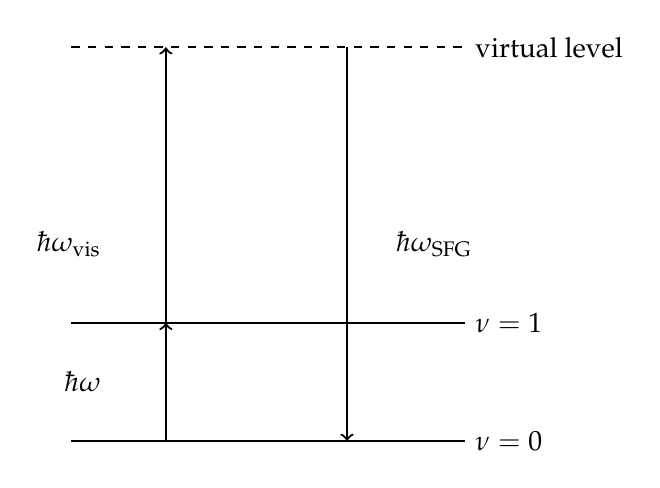
\begin{tikzpicture}[help lines/.style={thin,draw=black!50}]
%%\draw[help lines] (0,0) grid (4,4);
\draw [-, thick] (0,0) -- (5,0) node [anchor = west] {$\nu =0$};
\draw (0.5,0.75) node [anchor = east] {$\hbar\omega$};
\draw [-, thick] (0,1.5) -- (5,1.5) node [anchor = west] {$\nu = 1$};
\draw (0.5,2.5) node [anchor = east] {$\hbar\omega_{\text{vis}}$};
\draw [-, thick,dashed] (0,5) -- (5,5) node [anchor = west] {virtual level};
\draw (4.0,2.5) node [anchor = west] {$\hbar\omega_{\text{SFG}}$};
\draw [->, thick] (1.2,0) -- (1.2,1.5);
\draw [->, thick] (1.2,1.5) -- (1.2,5);
\draw [->, thick] (3.5,5) -- (3.5,0);
\end{tikzpicture}
\caption{The schematic of the VSFG process which involves IR and Raman transitions. The $\nu =0$, $\nu=1$ levels denote the ground and the first excited state of the oscillator, respectively.
 The dashed line denotes a virtual electronic state in the Raman transition.}\label{fig:sfg_1a}
\end{figure}

Because experiments usually employed visible and SFG frequencies are far from resonant 
conditions, $\chi^{(2),\text{NR}}$ can be considered totally off-resonant and therefore 
insensitive to the laser beams' frequencies involved. Therefore, we can neglect the 
frequency dependence of the non-resonant term.
The molecular information is contained in the resonant signal. The resonant susceptibility $\chi^{(2),\text{R}}(\omega)$ is given by 
\begin{equation}
  \chi_{\eta\xi\kappa}^{(2),\text{R}}(\omega)=\frac{-i}{\hbar}\int_0^\infty dt e^{i\omega t} \text{Tr}{[\rho,\mu_\kappa]\alpha_{\eta\xi}(t)},
\label{eq:chi_R}
\end{equation}
where the index $\eta$, $\xi$ and $\kappa$ are one of $x, y$ and $z$ labels of the laboratory coordinate frame.
In Eq.\thinspace(\ref{eq:chi_R}) $\rho=e^{-\beta H/Z}$ for a system with Hamiltonian $H$ and partition function $Z$ at reciprocal temperature $\beta=1/k_BT$;
$\mu_\kappa$ is the $\kappa$-th component of the system electric dipole and ${\alpha_{\eta\xi}}$ is the $\eta\xi$-th component of the polarizabiltiy tensor. [\cite{1995SM}]
Besides the vibrational resonance, $\chi^{\text{(2),R}}$, which reflects the vibrational and orientational characteristics of the surface species, 
the VSFG signal also includes the contribution from the non-resonant signal background $\chi^{\text{(2),NR}}$, 
due to static hyperpolarizability of the interface itself. [\cite{Che12}]  
For example, there are strong non-resonant second-order nonlinear responses [\cite{Pradier11,Vanselow12,Wieckowski99}] of the interface in the case of some metal(-oxide). 
Generally, experiments employ visible light and VSFG frequencies far from resonant conditions, therefore, the non-resonant 
term $\chi^{\text{(2),NR}}$ is approximately off-resonant to the light frequencies involved. [\cite{Morita02}]
%Neglecting the frequency dependence of the nonresonant term $\chi^{\text{(2),NR}}$ is usually a good approximation. 

\paragraph{Microscopic Expression of Molecular Hyperpolarizability} 
As the electric field is increased, the description of the induced dipole moment 
$\boldsymbol \mu$ should include the normally insignificant nonlinear terms. We can express the induced dipole moment as
\begin{equation}
  {\boldsymbol \mu} = {\boldsymbol \mu}_0 +\alpha {\bf E} + \beta {\bf E E}.
\label{eq:induced_mu}
\end{equation}
%or
%\begin{equation}
%  \mu_i = (\mu_0)_i +\alpha_i  E_i + \beta_{ijk}E_j E_k + \cdots.
%\label{eq:induced_mu}
%\end{equation}
The VSFG spectra are determined by the frequency-dependent hyperpolarizability in molecular level description. 
The frequency-dependent hyperpolarizability can be expressed as a sum of resonant and non-resonant terms:
\begin{equation}
\beta_{\eta\xi\kappa}(\omega_{\text{SFG}},\omega_{\text{vis}},\omega)=\beta_{\eta\xi\kappa}^{\text{R}}+\beta_{\eta\xi\kappa}^{\text{NR}},
\label{eq:beta}
\end{equation}
where $\eta$, $\xi$ and $\kappa$ are space-fixed axes.
The resonant term of the frequency-dependent hyperpolarizability is 
\begin{equation}
  \beta_{\eta\xi\kappa}^{\text{R}}(\omega_{\text{SFG}},\omega_{\text{vis}},\omega)=\sum_{v',v}\frac{\langle v|\alpha_{\eta\xi}|v'\rangle\langle v'|\mu_{\kappa}|v\rangle}{(\omega_{v'}-\omega_v)-\omega-i\gamma_{v'v}}\rho_v,
\label{eq:beta_R}
\end{equation}
where the subscripts $\eta$, $\xi$ and $\kappa$ denote body-fixed axes,
$\omega_{v'}-\omega_v$ is the vibrational energy gap, 
$\rho_v$ is the thermal distribution function of the initial vibrational states $v$,
$\alpha_{\eta\xi}$ is the $\eta\xi$-th component of the molecular dipole polarizability,
$\mu_{\kappa}$ is the $\kappa$-th component of the molecular dipole moment,
and $\gamma_{v'v}$ is the damping rate.
Since  
(see Appendix \ref{calculation_of_chi}) 
\begin{align}
\int_0^\infty dt e^{-it((\omega_{v'}-\omega_v)-\omega-i\gamma_{v'v})}=\frac{-i}{(\omega_{v'}-\omega_v)-\omega-i\gamma_{v'v}},
\label{integral_identity1a}
\end{align}
we can rewrite Eq.\thinspace(\ref{eq:beta_R}) as 
\begin{align}
  \beta_{\eta\xi\kappa}^{\text{R}}&=i\int_0^\infty dt \sum_{v'v}e^{-i[(\omega_{v'}-\omega_v)-\omega-i\gamma_{v'v}]t} \langle v|\alpha_{\eta\xi}|v'\rangle\langle v'|\mu_{\kappa}|v\rangle \rho_v \nonumber\\
   &=i\int_0^\infty dt \sum_{v'v}e^{i\omega t} \langle v|e^{iHt}\alpha_{\eta\xi}e^{-iHt}|v'\rangle\langle v'|\mu_{\kappa}|v\rangle \rho_v \nonumber\\
   &=i\int_0^\infty dt e^{i\omega t} \langle\alpha_{\eta\xi}(t)\mu_{\eta\xi}(0)\rangle,
\label{eq:beta_R_b}
\end{align}
where $H$ is the Hamiltonian of the system without external field. 
Eq.\thinspace(\ref{eq:beta_R_b}) indicates that the resonant term $\beta_{\eta\xi\kappa}^{(2),\text{R}}$ is the Fourier-Laplace transformation of the quantity $\langle\alpha_{\eta\xi}(t)\mu_{\kappa}(0)\rangle$, i.e., the ensemble average of the time correlation function $\alpha_{}(t)\mu_{r}(0)$.
The damping rate $\gamma_{v'v}$ is not explicitly included in Eq.\thinspace(\ref{eq:beta_R_b}), because the dephasing is incorporated in the time development of the off-diagonal matrix elements 
of $\alpha_{\eta\xi}(t)$ and $\mu_{\kappa}(0)$.

The $\chi^{(2),R}_{\eta\xi\kappa}$ is microscopically represented as the average sum of first-order hyperpolarizability of the constituent molecules $\beta$ in the space-fixed frame
\begin{align}
  \chi^{(2),R}_{\eta\xi\kappa} = \langle \sum_i^N \sum_{pqr} D_{\eta p}(\Omega_i) D_{\xi q}(\Omega_i) D_{\kappa r}(\Omega_i) \beta_{pqr}\rangle
\label{average_sum}
\end{align}
where $D(\Omega_i)$ is the direction cosine matrix of the $i$-th molecule, projecting $\beta$ onto the space-fixed frame. [\cite{Morita2000}]

%and evaluate it with the static hyperpolarizability, which can be calculated by an \abinitio Molecular Orbital (MO) package\cite{Morita02}, 
%\begin{equation}
%        \beta_{\eta\xi\kappa}^{\text{NR}}=\sigma\beta_{\eta\xi\kappa}^{\text{static}},
%\label{eq:beta_NR}
%\end{equation}
%where $\sigma$ is the symmetry number among the indices $\eta$, $\xi$ and $\kappa$.
%\paragraph{Derive the value of $\sigma$}
%The frequency-dependent hyperpolarizability, $\beta(\omega_1,\omega_2,\omega_3)$, satisfies the following equation 
%\begin{equation}
%\label{eq:beta_condition}
%        P_p(\omega_1)=\sum_q\alpha_{pq}(\omega_1)E_q(\omega_1)+\sum_{qr}\beta_{pqr}(\omega_1,\omega_2,\omega_3)E_q(\omega_2)E_r(\omega_3)+\cdots
%\end{equation}
%where the suffices $p$, $q$ and $r$ range over $x$, $y$ and $z$, and $P_p(\omega_1)$ is the induced dipole moment at frequncy $\omega_1$. The static polarizability and hyperpolarizability are defined as 
%\begin{equation}
%        \alpha_{pq}^{\text{static}}=(\frac{\partial P_p}{\partial E_q})_{E=0},\ \
%        \beta_{pqr}^{\text{static}}=(\frac{\partial^2 P_p}{\partial E_q \partial E_r})_{E=0}
%\label{eq:beta_condition}
%\end{equation}
%and thus the dipole moment in a static exteral electric field is expressed as 
%\begin{equation}
%        P_p^{\text{static}}=(P_p)_{E=0}+\sum_q\alpha_{pq}^{\text{static}}E_q+\frac{1}{2}\sum_{qr}\beta_{pqr}^{\text{static}}E_qE_r+\cdots,
%\label{eq:static_dipole_moment}
%\end{equation}
%where $(P_p)_{E=0}$ is the permanent dipole moment. From Eq. (\ref{eq:beta_condition}) and Eq. (\ref{eq:static_dipole_moment}), we obtain $\sigma=1/2$ in Eq. (\ref{eq:beta_NR}).

\paragraph{The Fresnel Factors}
Because of screening and dipole-dipole coupling, the local electric fields felt by molecules is different from the macroscopic fields. [\cite{Vanselow12}] 
The SFG signal depends on the magnitude of the local electric fields  of the the interacting optical beams at the interfaces. 
While the magnitude of the local electric fields is related to both the intensity of the incident beams and the linear refractive indices 
of the different layers (bulk) of the sample.  [\cite{Khatib16}] The Fresnel coefficients define the magnitude of the electric fields at the interface. 
Therefore, to find out the magnitude of the local electric fields, we need to evaluate the Fresnel factors. 
The SFG intensity $I_{\text{SFG}}$, is proportional to the intensities of the incident visible and infrared beams, $I_{\text{vis}}$, $I$, 
and to the square of the second-order nonlinear susceptibilities,
$\chi_{\eta\xi\kappa}^{(2)}(\omega_{\text{SFG}})$, of the interface:
\begin{equation}
        \chi_{\eta\xi\kappa}^{(2)}(\omega_{\text{SFG}})\propto|\sum_{\eta,\xi,\kappa}L_{\eta\eta}(\omega_{\text{SFG}})\chi_{\eta\xi\kappa}^{(2)}(\omega_{\text{SFG}})L_{\xi\xi}(\omega_{\text{vis}})L_{\kappa\kappa}(\omega)|^2\text{sec}^2(\theta_{\text{SFG}})I_{\text{vis}}I
\label{eq:chi}
\end{equation}
where $\eta$, $\xi$, $\kappa$ are the Descartes coordinates of the reference frame;
$\omega_{\text{SFG}}=\omega_{\text{vis}}+\omega$ is the frequency of SFG beam; 
$L_{\eta\eta}$, $L_{\xi\xi}$ and $L_{\kappa\kappa}$ are the Fresnel coefficients; 
$\theta_{\text{SFG}}$ is the reflected angle of SFG beam with respect to the normal 
direction in the medium.

\subsection{Sum Frequency Generation Spectra from Velocity-Velocity Correlation Functions}
%To construct SFG spectrum of O-H stretching at the water/vapor interface and to ascertain the molecular origin of SFG spectrum, 
%quantum corrected time correlation function \cite{Morita02,Morita04} and instantaneous normal mode (INM) methods are used 
%by Perry and coworkers.\cite{Perry03} 
%For  water/vapor interface, the INM SFG spectrum is in agreement with the time correlatin function SFG spectrum. 
%This implies that motional narrowing effects play little role  in the interfacial line shape. The Shen group suggests that 
%the motional narrowing effects may be significant in the SPS geometry, where the "free O-H" stretching peak is greatly diminished.\cite{WeiX02}
%========================
%\section{solutions}
%Here we discuss the calculation of nonlinear susceptibility of water molecules at liquid/vapor interfaces.
%The SFG spectrum is proportional to the square of the nonlinear susceptibility of water molecules at the water/vapor interface. \cite{QD94}  
%Details:
In this paragraph I review the derivation an expression for the calculation of the sum frequency generation spectra of water interfaces that is
based on the projection of the atomic velocities on the local normal modes, such an approach permits one to obtain the SFG signals from suitable
velocity-velocity ACFs, reducing the computational cost to that of the accumulation of a molecular dynamics trajectory, and therefore cutting 
the overhead costs associated with the explicit calculation of the dipole and polarizability tensor. Moreover, the method permits to interpret 
the peaks in the spectrum in terms of local modes.
The components of the resonant term $\chi^{\text{(2),R}}_{\eta\xi\kappa}$ of the second order susceptibility can be calculated 
according to the classical formula [\cite{Morita02,Morita2008,Nihonyanagi2011}]
\begin{align}
  \chi^{\text{(2),R}}_{\eta\xi\kappa}&=\frac{-i}{k_{\text{B}}T \omega} \int_0^\infty dt e^{i\omega t}\left\langle \dot{A}_{\eta\xi}(t) \dot{M}_{\kappa}(0)\right\rangle 
 \label{eq:chi}
\end{align}
%\begin{align}
% \chi^{(2)}_{XXZ,R}&=\frac{i}{k_BT \omega} \sum\limits_j \int_0^\infty dt e^{i\omega t} \left \langle \frac{\partial A_{XX}}{\partial r_j} \frac{\partial M_Z}{\partial r_j}  \dot{r}_j(0) \dot{r}_j(t) \right\rangle
% \label{eq:chi2}
% \end{align}
where $k_{\text{B}}$ is the Boltzmann constant, $\omega$ is the frequency of the IR beam, ${\bf M}$ (${A}$) are the dipole 
moment (dipole polarizability) of the system, and $\left\langle\dots\right\rangle$ denotes the average over all starting time points. 
%The derivation of Eq.\thinspace(\ref{eq:chi}) is given in Appendix \ref{calculation_of_chi}.
 
 The total dipole moment and dipole polarizability derivatives for the system can be expressed in terms of the water and bond contributions:
\begin{align}
 \dot{A}&=\sum_{i=1}^N \sum_{\epsilon}\dot{\alpha}^{i,\text{l},\epsilon} \\ 
 \dot{{\bf M}}&=\sum_{i=1}^N \sum_{\epsilon}\dot{\mu}^{i,\text{l},\epsilon} 
 \label{eq:A-M}
\end{align}
where ${\mu}^{i,\text{l},\epsilon}$ (${\alpha}^{i,\text{l},\epsilon}$) is the dipole moment (polarizability)
of the bond $\epsilon$ of the $i$-th water molecule, the superscript (l) denote these quantities are measured in the 
lab frame, and $N$ is the total number of the water molecules.
Therefore, the correlation function in Eq.\thinspace(\ref{eq:chi}) can be written as 
\begin{align}
  \langle\dot{A}_{\eta\xi}(t)\dot{M}_{\kappa}(0)\rangle 
    &=\sum_{i=1}^N \sum_{\epsilon}\left\langle\dot{\alpha}_{\eta\xi,i,\epsilon}^{\text{l}}(t)\dot{\mu}_{\kappa,i,\epsilon}^{\text{l}}(0)\right\rangle \nonumber \\ 
    &+\sum_{i=1}^N \sum_{\epsilon}\left\langle\dot{\alpha}_{\eta\xi,i,\epsilon}^{\text{l}}(t)\dot{\mu}_{\kappa,i,-\epsilon}^{\text{l}}(0)\right\rangle \nonumber \\
    &+\sum_{i,j=1;i\neq j}^N \sum_{\epsilon,\epsilon'}\left\langle\dot{\alpha}_{\eta\xi,i,\epsilon}^{\text{l}}(t)\dot{\mu}_{\kappa,i,\epsilon'}^{\text{l}}(0)\right\rangle.
 \label{eq:correl_AM}
 \end{align}
In Eq.\thinspace(\ref{eq:correl_AM}), the first term of the right-hand side is the bond auto-correlation, the second term accounts 
for the correlation between the two bonds in the same water molecule, and the third them for the correlation between 
bonds in two different water molecules.
 
We assume that the bond elongation are small compared to the total bond length and stretching frequencies of the bond are 
much larger than frequencies of bond reorientation, for example, the libration.
Therefore, we can approximately write ${\dot\mu}(0)$ by 
\begin{align}
    \dot\mu_{\kappa}(0)&=\sum_i^{x,y,z}{\bf{D}}_{\kappa i}(0)\dot{\mu}_i(0) \nonumber \\
                       &=\sum_i^{x,y,z}{\bf{D}}_{\kappa i}(0)\biggl(\sum_j^{x,y,z}\frac{d\mu_i}{d r_j}\frac{d{r}_j}{dt}|_{t=0}\biggr) \nonumber \\
                       &=\sum_{i}^{x,y,z}{\bf{D}}_{\kappa i}(0)\frac{d\mu_i}{dr_z}v_z(0),
    \label{eq:dot_mu}
 \end{align}
where ${\bf D}_{\kappa i}$ is the direction cosine between the laboratory-fixed $\kappa$ axis and the molecular-fixed $i$ axis,
and $v_z=\frac{d{r}_z}{dt}|_{t=0}$ is the projection of the velocity on the bond axis.

Similarly, for the dipole polarizability, we have
\begin{align}
  \dot\alpha_{\eta\xi}(t)&=\sum_{i,j}^{x,y,z} \biggl({\bf{D}}_{\eta i}(t)\frac{\partial\alpha_{ij}}{\partial r_z}{\bf{D}}_{\xi j}(t)\biggr)v_z(t). 
  \label{eq:dot_alpha}
 \end{align}
The Eq.\thinspace(\ref{eq:dot_mu}) and Eq.\thinspace(\ref{eq:dot_alpha}) simplify the calculation of the  
$\left\langle \dot{A}_{\eta\xi}(t) \dot{\bf{M}}_{\kappa}(0)\right\rangle$ in Eq.\thinspace(\ref{eq:chi}), because $v_z(t)$
and ${\bf{D}}(t)$ can be readily determined from the DFTMD
trajectory, and $\frac{d\mu_i}{dr_z}$ and $\frac{d\alpha_{ij}}{dr_z}$ can be parameterized. [\cite{Corcelli05,Khatib16}]
%
\begin{figure}
\centering
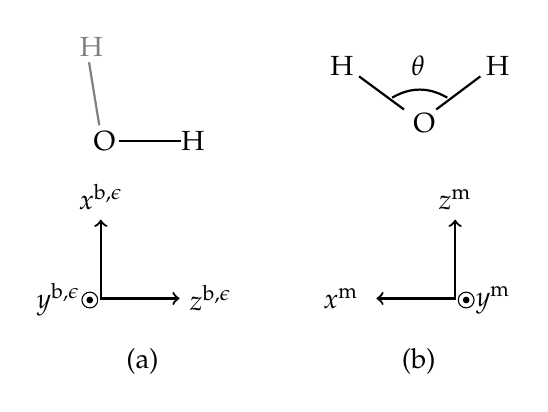
\begin{tikzpicture}[help lines/.style={thin,draw=black!50}]
%\draw[help lines] (0,0) grid (4,4);
%a
\draw [<->,thick] (0,1) node (xaxis) [above] {$x^{\text{b},\epsilon}$}
  |- (1,0) node (zaxis) [right] {$z^{\text{b},\epsilon}$};
  \filldraw[black] (-0.14,-0.02) circle (1pt) node [anchor=east] {$y^{\text{b},\epsilon}$};
\draw(-0.14,-0.02) circle (0.1);
\draw (0.2, -0.8) node [anchor=west] {(a)};
% H2O
\draw[gray,thick] (-0.02, 2.2) coordinate (a_1) -- (-0.15, 3) coordinate (a_2);
\draw[thick] (0.23, 2) coordinate (b_1) -- (1.02, 2) coordinate (b_2);
\draw (0.31, 2) node [anchor=east] {O};
\draw (0.9, 2) node [anchor=west] {H};
\draw[gray] (-0.12, 2.95) node [anchor=south] {H};
%\draw (0.56, 2.61) node {\chemfig{[:-84]H-O-[:0]H}};
%b
\draw [<->,thick] (3.5,0)--(4.5,0) node (xaxis){} 
  |- (4.5,0)--(4.5,1) node (zaxis) [above] {$z^{\text{m}}$};
  \filldraw[black] (4.64, -0.02) circle (1pt) node [anchor=west] {$y^{\text{m}}$};
\draw (2.7, 0) node [anchor=west] {$x^{\text{m}}$};
\draw(4.64,-0.02) circle (0.1);
\draw (3.7, -0.8) node [anchor=west] {(b)};
% H2O
\draw[thick] (3.85, 2.4) coordinate (a_1) -- (3.28, 2.82) coordinate (a_2);
\draw[thick] (4.26, 2.4) coordinate (b_1) -- (4.82, 2.82) coordinate (b_2);
\draw[thick] (3.7,2.55) to [out=30,in=150] (4.4,2.55);
\draw (4.03, 2.7) node [anchor=south] {$\theta$};
\draw (4.37, 2.23) node [anchor=east] {O};
\draw (5.04, 2.7) node [anchor=south] {H};
\draw (3.06, 2.7) node [anchor=south] {H};
%\draw (4.06, 2.61) node {\chemfig{[:-37]H-O-[:37]H}};
\end{tikzpicture}
  \caption{\label{fig:frameworks} The representation of the bond (a) and the molecular (b) frameworks.}
\end{figure}

%
We used three different frameworks: the lab framework ($x^{\text{l}},y^{\text{l}},z^{\text{l}}$), the molecular framework 
($x^{\text{m}},y^{\text{m}},z^{\text{m}}$) and the bond framework ($x^{\text{b}},y^{\text{b}},z^{\text{b}}$) (see Fig.\thinspace\ref{fig:frameworks} [\cite{Khatib2017}]).
In the lab framework, the $z^{\text{l}}$-axis is perpendicular to the interface. 
The molecular frame will be used to decompose the signal into normal modes of water monomers. 
For the $j$-th molecule, the $z^{\text m}$ axis is along the bisector of the H-O-H angle, the $x^{\text m}$ axis is in the molecular plane, 
and the $y^{\text m}$ axis is out of the molecular plane. [\cite{Khatib2017}] 

In the bond framework, $z^{\text{b},\epsilon}$ axis is along the bond $\epsilon$ of a molecule, $z^{\text{b},\epsilon}$
is in the molecular plane and $y^{\text{b},\epsilon}$ is out of the molecular plane.
\begin{align}
  \dot{\alpha}^{\text{l},\epsilon} &= {\bf{D}}^{\text{m}}{\bf{D}}^{\text{b},\epsilon}(\frac{\partial{\alpha}^{\text{b}}}{\partial r}\dot
    r^{\epsilon})({\bf D}^{\text{b},\epsilon})^{\text{T}}({\bf D}^{\text{m}})^{\text{T}}, \\ 
    \dot\mu^{\text{l},\epsilon} &= {\bf{D}}^{\text{m}}{\bf{D}}^{\text{b},\epsilon}(\frac{\partial \mu^{\text{b}}}{\partial r}\dot r^{\epsilon}).
    \label{eq:dot_mu-alpha}
 \end{align}
The direction cosine matrix ${\bf{D}}^{\text{b},\epsilon=1}$ and ${\bf{D}}^{\text{b},\epsilon=-1}$ can be expressed as 
\begin{equation}
    {\bf{D}}^{\text{b},1}=\left(
                \begin{matrix}
                    \text{cos}\frac{\theta}{2} &  0  & -\text{sin}\frac{\theta}{2}\\
                    0 & 1 & 0\\
                    \text{sin}\frac{\theta}{2} & 0 & \text{cos}\frac{\theta}{2}
\end{matrix}
\right),\quad
    {\bf{D}}^{\text{b},-1}=\left(
         \begin{matrix}
             -\text{cos}\frac{\theta}{2} & 0 & \text{sin}\frac{\theta}{2}\\
             0 & 1 & 0\\
             \text{sin}\frac{\theta}{2} & 0  & \text{cos}\frac{\theta}{2}
\end{matrix}
\right),
\label{eq:D_b}
\end{equation}
where $\theta$ is the H-O-H angle in a water molecule.
%The approximate value of the angle is 105.5$^\circ$.
We can use ${\bf{D}}^{\text{m}}$ to transform the coordinates in a molecular framework to coordinates in the lab framework. 
Because the orientation of water molecules is changing during the simulation, 
%the angle $\theta'_i$ between the water dipole moment and the $z$-axis is time dependent, therefore, 
${\bf{D}}^{\text{m}}$ is time dependent. 
%It can be expressed as 
%\begin{equation}
%    {\bf{D}}^{\text{m}}=
%    \left(
%        \begin{matrix}
%            \text{cos}{\gamma} & \text{sin}{\gamma} & 0\\
%            -\text{sin}{\gamma} & \text{cos}{\gamma} & 0\\
%            0 & 0 & 1
%        \end{matrix}
%     \right)
%     \left(
%         \begin{matrix}
%             \text{cos}{\theta'} & 0 & -\text{sin}{\theta'}\\
%             0 & 1 & 0\\
%             \text{sin}{\theta'} & 0  & \text{cos}{\theta'}
%         \end{matrix}
%     \right) 
%     =
%     \left(
%         \begin{matrix}
%             \text{cos}{\gamma}\text{cos}{\theta'} & \text{sin}{\gamma} & -\text{cos}{\gamma}\text{sin}{\theta'}\\
%             -\text{sin}{\gamma}\text{cos}{\theta'} & \text{cos}{\gamma} & \text{sin}{\gamma}\text{sin}{\theta'}\\
%             \text{sin}{\theta'} & 0  & \text{cos}{\theta'}
%         \end{matrix}
%     \right),
%\label{eq:D_m}
%\end{equation}
%where $\gamma$ is the angle between the incident plane (x-z plane) and the molecular plane of a water molecule,
%and $\theta'$ is the angle of the dipole moment of the water molecule from the normal direction of the interface, 
%and both $\gamma$ and $\theta'$ are time dependent.

The parametrization of $\frac{\partial \mu_{k}}{\partial r_z}$ and $\frac{\partial\alpha_{ij}}{\partial r_z}$ is based 
on the calculation of Maximally Localized Wannier Functions (MLWF) [\cite{Marzari97}] 
 and can be done through the approach developed by Salanne \etal [\cite{Salanne08}] and Khatib \etal [\cite{Khatib2017}]
The main advantage of such approximation for the calculation of the susceptibility is that still retain details of the
water/vapor interfaces including the full electronic structure, but its computational
cost is reduced with respect to a full calculation with the instantaneous evaluation of the 
molecular dipoles and polarizabilities. [\cite{sulpizi2013}] 
The implementation of this parametrization is given in Appendix \ref{calculate_derivatives}.
%\paragraph{Calculation of $\chi^{(2)}$ (Method 2)}
%We now consider the velocities projection on the water normal modes, identified by the collective variables ${\bf{R}}_j$ in the molecular framework. 
%The single water molecule has nine normal modes. Six of them have the angular frequencies $\omega$ equal zero and three normal modes remains. 
%The three normal modes are the symmetric stretching (SS), the antisymmetric stretching (AS) and the bending (B).
%The dipole moment and the molecular polarizability of the $i$th water molecule can be rewritten as
%\begin{align}
%    \dot{\bf \alpha}_{i}^{\text{l}}(t)&={\bf{D}}_{\text{m},i}(\sum_{j=Q,SS,AS}\frac{\partial{\bf\alpha}_{i}^{\text{m}}}{\partial R_j}){\bf{D}}^{\text{T}}_{\text{m},i}, \\ 
%    \dot{\bf \mu}_{i}^{\text{l}}&={\bf{D}}_{\text{m},i}(\sum_{j=Q,SS,AS}\frac{\partial{\bf\mu}_i^{\text{m}}}{\partial R_j}\dot{R}_j).  
%    \label{eq:dot_mu_alpha}
%\end{align}
%where $i$ denote the $i$-th water molecule.
%To parametrize the derivatives $\frac{\partial \alpha_i^{\text{m}}}{\partial R_j}$ and $\frac{\partial {\bf{\mu}}_i^{\text{m}}}{\partial R_j}$,
%the Maximally Localized Wannier Functions (MLWF) were emplyed.\cite{Salanne08,Khatib2017}
 
\chapter{Experimental SFG spectra of salty interfaces}\label{CHAPTER_SFG_Exp}
In this chapter, we will give the experimental results obtained on salty solutions containing alkali cations and nitrate (iodide) anions. [\cite{PS03,AJ12,HuaWei2014}] 

%We will choose the interface of lithium nitrate solution as our research object, which is a typical example of the interface of alkali metal nitrate solution.
From the experimental data of surface tension dependence on solute concentration $\text{d}\gamma/\text{d}m_2$ 
at low electrolyte concentrations ($\leq$1.5 M ), [\cite{Weissenborn95,Hey81,Jarvis68,Jarvis72}] 
%and the assumption that \Na is the most excluded cation
the relation of the surface/bulk molar concentration ratio $K_{\text{p}}$ [\cite{Pegram06}] among \li, \Na and \K is: 
\begin{equation}
0=K_{\text{p,Na}^+}< K_{\text{p,K}^+}< K_{\text{p,Li}^+}.
\label{eq:bscr}
\end{equation}
i.e., \Na is the most surface-excluded in the water solution RNO$_3$, \K is less excluded, 
and \Li is the least excluded cation.
In modeling the interfaces of aqueous sulitons of alkali metal nitrates, we decided to start with LiNO$_3$, because the $Li^+$ ion is the least excluded of the vapor-liquid interface 
among the alkali metal ions. 
%
%The aim of our work here is to provide a molecular picture 
%for the water/vapor interface of the \ch{LiNO3}-containing solution 
%to interpret the experimental spectra. In particular a question raises if simple models 
%for the solvated ion clusters can already provide information
%on the ions-water complexes formed at the interface. 
%It is known that nitrate (\nitrate) is a naturally occurring ion which is part of the nitrogen cycle, 
%and it can reach both surface water and groundwater as a consequence of agricultural activity. 
%Nitrate also has effects on human health,  because of the toxicity caused by its reduction to nitrite (NO$_2^-$). \cite{WHO11}
%The biological effect of nitrite in humans is its involvement in the oxidation of
%normal Hb to metHb, which is unable to transport oxygen to the tissues.
%For example, infants who drink water with high levels of nitrate (more than 10 mg/L) may suffer 
%a serious health condition due to blue baby syndrome.\cite{Knobeloch00}
%

%The goal of this chapter is to find the origin of the main characteristics of the VSFG spectra of the \LiN solution,
%and provide a molecular picture to interpret the recorded spectra.
%In order to achieve this goal, we simulate water/vapor interface including \Li and \nitrate, 
%as shown in Fig.\thinspace\ref{fig:interface_chandler},
%and extract the vibrational spectroscopic properties of the water/vapor interface of LiNO$_3$ solution.
%=========
%
%\begin{figure}[htbp]
%\centering
%\includegraphics [width=0.5 \textwidth] {./diagrams/interface_chandler}
%\setlength{\abovecaptionskip}{0pt}
%\caption{\label{fig:interface_chandler} The water/vapor interfaces of \LiN solution and pure water. 
%The right panel shows that the \Li and the \nitrate ions are separated by a water molecule at the salty interface.}
%\end{figure}
%The water molecules below 4 \AA  of the instantaneous interfaces are shown opaquely. 

%
Hua \etal [\cite{HuaWei2014}] have recently measured the VSFG spectra of water/vapor interface of \LiN salt solutions in the OH stretching region
(3000--3800 \centimeter) using Heterodyne Detected VSFG spectroscopy. [\cite{HuaWei2011,HuaWei2011b,ChenXiangKe2010}] 
The experimental result of the VSFG intensity of the alkali nitrate interfaces is given by in Fig.\space\ref{fig:Allen12}. 
At a difference with the spectra for the water interface, in the spectra of 
\LiN solutions, a depletion of the 3200 \cm peak is observed, with an 
enhancement of the 3400 \cm peak.
A similar behaviour had been observed for the interface of NaNO$_3$ and 
Mg(NO$_3$)$_2$ solutions. [\cite{AJ12,HuaWei2014}] It has been 
suggested that this depletion of the 3200 \cm peak, and in some cases 
the enhancement of the 3400 \cm peak, is an indication that nitrate 
ions reside at the interface. On the other hand the small 
cations should have little surface propensity. 
It has also been argued that the positive electric field found at the interface of NaCl, NaI and 
NaNO$_3$ salt solutions is due to the formation of an ionic double layer 
between anions located near the surface and their counter-cations (e.g.
Na$^+$) located further below. In Phase-Sensitive (PS) VSFG experiments the 
magnitude of the induced change in the Im$\chi^{(2)}$ spectra comparatively
to that of the neat water suggested that \nitrate has a surface propensity 
just in between I$^-$ and Cl$^-$. [\cite{Verreault2013,Verreault2009}] 
% exp. results.
\begin{figure}[H] %[htbp]
\centering
  \includegraphics [width=0.6 \textwidth] {./diagrams/vsfg_alkali_nitrate}
\setlength{\abovecaptionskip}{0pt}
  \caption{\label{fig:Allen12}Experimental VSFG intensity of \LiN solutions, compared with that of neat water. [\cite{HuaWei2014}]}
\end{figure}

%\begin{figure}[htbp]
%    \centering
%    \begin{tikzpicture}
%        \begin{axis}[
%        scale=0.8, % scale the figure but the labels
%        /pgf/number format/.cd,
%        %use comma,
%        1000 sep={}, % separator of thousands
%        legend style={draw=none},
%        legend pos=north west,
%        %title=VSFG Intensity,
%        xlabel={Wave Number (cm$^{-1}$)},
%        every axis x label/.style={
%        at={(rel axis cs: 0.5, -0.20)},
%        anchor=center}, 
%        ylabel={Intensity (Arb. Unit)},
%        every axis y label/.style={    
%        at={(rel axis cs:-0.18, 0.5)},rotate=90,
%        anchor=center}, 
%        ymin=0,
%        ymax=0.3,
%        minor y tick num=1,
%        ]
%        \addplot[mark=x, black,domain=3000:3800,very thick]table{./chapters/chap4/data/Net_water.dat};
%        \addlegendentry{Neat Water}
%        \addplot[mark=*, blue,domain=3000:3800,very thick]table{./chapters/chap4/data/LiNO3.dat};
%        \addlegendentry{1M  \LiN}
%      \end{axis}
%   \end{tikzpicture}
% \setlength{\abovecaptionskip}{0pt}
%  \caption{\label{fig:Allen12}Experimental VSFG intensity of \LiN solutions, compared with that of neat water.\cite{HuaWei2014}}
% \end{figure}

  \chapter{Alkali Nitrate Clusters}\label{CHAPTER_results_clusters}
  In this chapter, gas phase clusters including alkali cations, nitrate ions and a few water molecules have been used to understand the
  effects of alkali cations and nitrate anions on hydrogen
  bonding. [\cite{jiangling2010,heine2015}] 
  VDOS is used to extract the vibrational signatures for the water molecules in these systems.
  In the first two paragraphs the effect of the anion and the cation are separately investigated. 
  The two clusters, NO$_3^-$(H$_2$O)$_3$ and \li(H$_2$O)$_4$, are used 
  to study the structural and dynamical properties of water clusters with nitrate ions and with alkali cations at $T= 300$ K. 
  In paragraph \ref{paragraph_clusters_alkali_nitrate_and_water_molecules}, the effects of the alkali metal cations 
  and the nitrate anion are discussed within clusters containing both cations and anions and an increasing number of water molecules.
  %
  \section{Cluster of Nitrate and Water Molecules}\label{paragraph_3w_nitrate}
  %EXAMPLE of FORMULA
  %$$X_n=X_k \qquad\hbox{if and only if}\qquad Y_n=Y_k \quad\hbox{and}\quad Z_n=Z_k.$$
  
  %\begin{wrapfigure}{l}[0.05cm]{8.0cm}
  %\centering
  %\includegraphics[width=0.3\textwidth]{./diagrams/3_NO3_small}
  %\setlength{\abovecaptionskip}{10pt}
  %\caption{The geometry optimized structure of the cluster NO$_3^-$(H$_2$O)$_3$. The red dotted lines denote the H-bonds.}\label{fig:3_NO3_small}
  %\end{wrapfigure}
  \begin{figure}
  \centering
  \includegraphics[width=0.5\textwidth]{./diagrams/clusters_4}
  \setlength{\abovecaptionskip}{0pt}
    \caption{\label{fig:clusters_4}The geometry optimized structure of the clusters: (a) NO$_3^-$(H$_2$O)$_3$; (b)RNO$_3$(H$_2$O)$_3$; (c) RNO$_3$(H$_2$O)$_4$; (d) RNO$_3$(H$_2$O)$_5$ (R=Li,Na,K). More structural properties are shown in Appendix \ref{structure_of_clusters}.}
  \end{figure}
  First, we consider the water cluster with a nitrate ion, NO$_3^-$(H$_2$O)$_3$. The symmetric isomer of the cluster, 
  as shown in Fig.\thinspace\ref{fig:clusters_4}(a), is obtained by geometry optimization at the BLYP/TZV2P level of theory. 
  According to the definition of the H-bond, [\cite{JT90,SB02}] there are three H-bonds in it,
  i.e., only one of the two OH bonds is H-bonded to \nitrate in each water molecule. 
  Therefore, for each water molecule, we say there is one HB and one quasi-HB.
  %The three water molecules in the cluster NO$_3^-$(H$_2$O)$_3$ have similar dynamical properties.
  Therefore, the two OH bonds in each water molecule exhibit different vibrational features. 
  Fig.\thinspace\ref{fig:vdos_NO3-3w_2_H6H7} shows the difference of VDOS for the OH bonds in the cluster.
  %(MS:repetition)It shows that both H atoms have two vibrations modes, but the two H atoms in a water molecule in the cluster prefer to vibrateing differently.
  For each water molecule, one OH bond is vibrating in the frequency range 3680--3700 cm$^{-1}$, 
  while the other in the frequency range 3380--3440 cm$^{-1}$. 
  The difference of frequencies between the vibrational modes is about $\Delta\nu=$ 250 \centimeter.
  %
  \begin{figure}[b!] %[htbp]
  \centering
  \includegraphics [width=0.6\textwidth] {./diagrams/vdos_NO3-3w_2_H6H7_simple}%
  \setlength{\abovecaptionskip}{0pt}
    \caption{\label{fig:vdos_NO3-3w_2_H6H7} The VDOS for the two OH bonds in w1 (Fig.\thinspace\ref{fig:clusters_4}(a)) of NO$_3^-$(H$_2$O)$_3$.} 
    %The length of the DFTMD trajectory is 5 ps.
  \end{figure}  %(Calculated from the function vdos3.f and ft$\_$5s.sh)
  %(MS:repetition)A quasi-HB is formed if the O--H distance $r_\text{OH}$ satisfies the condition $r_\text{OH}<3.5$ \AA, but not that the O--H$\cdots$O angle is less than $\frac{\pi}{6}$. \cite{JT90} 
  Additionally, we label the three water molecules as w1, w2, and w3, respectively (Fig.\thinspace\ref{fig:clusters_4}(a)). 
  For the three water molecules, we can find some difference in the structural parameters.
  Table\thinspace\ref{tab:3_nitrate_bond} gives the calculated lengths of H-bonds in the cluster NO$_3^-$(H$_2$O)$_3$. 
  The average differences $\Delta{d}$ between the H-bonds and the quasi-H-bonds are 0.69 \AA (Table\thinspace\ref{tab:3w_nitrate}). 
  %\paragraph{Lengths of Hydrogen Bonds}
  %[(I deleted this paragraph, because now i am not sure on this idea.) To find the possible source of the different 
  %vibrational features of water molecules in the clusterNO$_3^-$(H$_2$O)$_3$, we considered the structural properties and VDOS for water molecules in this cluster. 
  %=============
  %\begin{table}
  %\centering
  %\caption{\label{tab:3_nitrate_bond}%
  %The lengths of H-bonds in the cluster NO$_3^-$(H$_2$O)$_3$. The indices of H atoms: H6, H7 in w1; H9, H10 in w2 and H12, H13 in w3.} 
  %\begin{tabular}{ccc} \\\toprule
  % HBs& $r_a\pm\delta$ (100 K)(\A) & \multicolumn{1}{c}{ $r_a\pm\delta$ (300 K)}(\A)\\
  %\hline
  % H6-O2 &2.75$\pm$0.62& 2.40$\pm$0.52 \\
  % H7-O4 &2.79$\pm$0.58& 3.02$\pm$0.72 \\
  % H9-O3 &2.89$\pm$0.60 &2.56$\pm$0.48 \\
  % H10-O4 &2.74$\pm$0.49&3.20$\pm$0.41 \\
  % H12-O3 &2.46$\pm$0.45&2.29$\pm$0.47 \\
  % H13-O2 &2.75$\pm$0.59 &3.11$\pm$0.72
  %\end{tabular}
  %\end{table}
  %===================
  %\begin{figure}[htbp]
  %\centering
  %\includegraphics [width=0.5\textwidth] {./diagrams/gdr_ON-wat--3_NO3_Sans} 
  %\setlength{\abovecaptionskip}{20pt}
  %\caption{\label{gdr_ON-wat--3_NO3_Sans}The nitrate O ($\text{O}_\text{n}$)--water O ($\text{O}_\text{w}$) and nitrate O--water H ($\text{H}_\text{w}$) RDFs for the cluster NO$_3^-$(H$_2$O)$_3$.
  %The peaks for the former are 1.93, 2.95 and 3.95 \A, and for the later are 2.95 and 4.80 \A.}
  %\end{figure} 
  %==================================================================================
  %When $T=300$ K, the difference $r_a$ between different hydrogen atoms in one water molecule is
  %$\Delta{r_a}=0.69$ \AA, while $\Delta{r_a}=0.13$ \AA for $T=100$ K.
  %It shows that the vibrational peaks for the three water molecules are much closer than that at the higher temperature 300 K. 
  %
  %The calculated VDOS for water molecules in the cluster 
  %at a lower temperature 100 K is given in Fig.\thinspace\ref{fig:vdos_LiNO3-3w_100K_w1-2-3_font35}. 
  %At the lower temperature,
  %the 3 water molecules are more symmetric distributed bound to the central nitrate.
  %Therefore, the difference between H-bonds in the symmetric isomer of NO$_3^-$(H$_2$O)$_3$ is likely a finite temperature effect, which can be verified by the calculation of the VDOS for water molecules.
  %
  %Both differences $\Delta\nu$ and $\Delta{d}$ decrease as the temperature decrease,
  %Therefore, the different vibrational features are temperature-dependent effect. 
  %--------------------
  %\begin{figure}[htbp]
  %\centering
  %\includegraphics [width=0.5 \textwidth] {./diagrams/vdos_LiNO3-3w_100K_w1-2-3_font35} 
  %\setlength{\abovecaptionskip}{20pt}
  %\caption{\label{fig:vdos_LiNO3-3w_100K_w1-2-3_font35} The VDOS $g(\nu)$ for water 
  %molecules in the cluster NO$_3^-$(H$_2$O)$_3$ at 100 K shows that 
  %the vibrational peaks for the three water molecules are very close to each other ($\Delta\nu <$ 10 \cm)for both vibrational and bending modes.}
  %\end{figure}
  %====================================================================================
  %In addition, the VDOS for H atoms and water molecules in NO$_3^-$(H$_2$O)$_3$ (Fig.\thinspace\ref{fig:vdos_NO3-3w_2_H-wat}) shows that H's contribution dominates that of the water molecule. 
  %\begin{figure}[htbp]
  %\centering
  %\includegraphics [width=0.5\textwidth] {./diagrams/vdos_NO3-3w_2_H-wat}%
  %\setlength{\abovecaptionskip}{20pt}
  %\caption{\label{fig:vdos_NO3-3w_2_H-wat}The comparison between the VDOS for H and of a whole water molecule, for a water molecule ({w1}, Fig. ~\ref{fig:3_NO3_small}), 
  %in NO$_3^-$(H$_2$O)$_3$ at 300 K.}
  %\end{figure}  %(Calculated from the function vdos3.f and ft$\_$5s.sh)
  %============
  %section 4_Li
  %============
  \section{Cluster of Alkali Metal Cation and Water Molecules}
  \begin{wrapfigure}{l}[0.05cm]{6.5cm}
  \centering
  \includegraphics[width=0.25\textwidth]{./diagrams/4_Li}
  \setlength{\abovecaptionskip}{0pt}
  \caption{\label{fig:4_Li}The cluster Li$^+$(H$_2$O)$_4$.}
  \end{wrapfigure}
  %====
  To find the effects of alkali cations on the structural properties of water, we investigate the cluster \li(\wat)$_4$ 
  (Fig.\thinspace\ref{fig:4_Li}). We concentrate on two aspects: the radial distribution function (RDF), 
  and the VDOS for water molecules of this cluster.

  The sharp peaks in the RDF given in Fig.\thinspace\ref{gdr_4_Li} show that the solvation shell of \Li is bound to all the four water molecules.
  The peak for $g_{\text{LiO}}$ is at 2.02 \AA, and for $g_{\text{LiH}}$ is 2.69 \AA. 
  \begin{figure}[b!]
  \centering
  \includegraphics[width=0.6\textwidth] {./diagrams/gdr_4_Li}
  \setlength{\abovecaptionskip}{0pt}
    \caption{\label{gdr_4_Li} The RDFs $g_{\text{Li-O}}$ and $g_{\text{Li-H}}$ for the cluster \li(H$_2$O)$_4$.} 
  \end{figure}
  %
  \begin{figure}[htbp]
  \centering
  \includegraphics [width=0.6\textwidth] {./diagrams/vdos_4_Li} 
  \setlength{\abovecaptionskip}{0pt}
  \caption{\label{vdos_4_Li} %old version: vdos_4_Li-wat_2p 
    The VDOS for the four water molecules (all water molecules) in the cluster \li(\wat)$_4$.} 
  %(a) The VDOS for all water molecules (black line), Li-bound (red) and H-bonded water molecules (blue).
  %(b) The VDOS for H-bonded water molecules (blue), and of both Li-bound and H-bonded water molecules (orange). }
  \end{figure}
  %

  The VDOS for water molecules in the cluster \li(\wat)$_4$ is calculated from a 20-ps trajectory,
  during which one water molecule escaped from the bonding of the \Li and then formed a new HB to 
  another water molecule. First, Fig.\thinspace\ref{vdos_4_Li} 
  shows that, in this case, there are two types of OH stretching modes in \li(\wat)$_4$ cluster:
  free OH stretch which peaks at 3705 \cm and bonded OH stretch at 3625 \centimeter. 
  However, the water molecules just bound to \Li has two degenerate free O-H stretching modes. 
  %Second, Fig.\thinspace\ref{vdos_4_Li}  shows that if a H-bonded water molecule is in the solvation shell of \Li, 
  %the H-bonded OH streching frequency is 75 \cm higher than that of the H-bonded OH strech outside the solvation shell of \Li. 
  %
  \begin{figure}[htbp]
  \centering
  \includegraphics [width=0.6 \textwidth] {./diagrams/vdos_4_Li-wat_w1_5ps} 
  \setlength{\abovecaptionskip}{20pt}
  \caption{\label{vdos_4_Li-wat_w1_5ps} 
    The VDOS for the water molecules bound to Li$^+$ (three water molecules) 
    in the cluster \li(\wat)$_4$.} 
  \end{figure}
  %
The VDOS for water molecules only bound to \Li (Fig.\thinspace\ref{vdos_4_Li-wat_w1_5ps}) shows that these water molecules only have free OH stretch, 
  since there is only a broad stretching mode at 3705 cm$^{-1}$.

  \section{Clusters of Alkali Nitrate and Water Molecules}\label{paragraph_clusters_alkali_nitrate_and_water_molecules}
  %\begin{wrapfigure}{r}[0.05cm]{7.5cm}
  %\centering
  %\includegraphics[width=0.3\textwidth]{./diagrams/3_RNO3}
  %\setlength{\abovecaptionskip}{10pt}
  %\caption{\label{fig:3_RNO3}The clusters RNO$_3$(H$_2$O)$_3$ (R=Li, Na, K).}
  %\end{wrapfigure}
  %===================
  %MS:INSERT AN INTRO:
  %===================
  As a first minimal model system for the interfaces of alkali nitrate solution, we consider alkali nitrate water clusters including 3 to 5 waters. 
  The idea is to investigate the effect of the alkali nitrate on the vibrational properties of those water molecules which are directly 
  H bonded to the ions.
  In our simulations, the clusters are geometry optimized and the most stable configurations are determined (Fig.\thinspace\ref{fig:clusters_4}(b)(c)(d)).
  The first interesting result is that for all the clusters containing 3 to 5 water molecules, a contact ion pair is maintained during the 
  300 K simulation trajectories where a direct interaction involves the cation and one of the nitrate oxygen's. 
  %The most stable isomer of the RNO$_3$(NO$_3$)$_3$ complex (R=Li,Na,K) is shown in Fig.~\ref{fig:clusters_4}(b) and compared to the symmetric slovation of the simple NO$_3$(H$_2$O)$_3$. 
  %Independently of the type of alkali cations (Li,Na,K), the most stable structure is the same.

In the LiNO$_3$(H$_2$O)$_3$ cluster, there are three H-bonds and three Li-O bonds. 
The average lengths of them are given in Table\thinspace\ref{tab:table_lino3}. 
We use HB1, HB2 and HB3 to denote the HB between w1 and w2, w2 and \nitrate, and w3 and \nitrate, 
respectively (Fig.\thinspace\ref{fig:clusters_4}(b)). Both the average lengths of HB1 and HB3 are very close 
to each other and both of them are smaller than those of HB2. 
Since both w1 and w2 are bound to \li, we calculate an average value $\bar{d}_{\text{HB}}=1.81$ \AA of the lengths of HB1 and HB3.
The difference between length of HB2 and $\bar{d}_{\text{HB}}$ is $\delta d_{\text{HB}}=0.19$ \AA.
By testing the difference of environment of each H-bonds,  we obtain that $\delta d_{\text{HB}}$ comes from the 
difference between Li-O  and H-bonds.
\begin{table}[htbp]
\centering
\caption{\label{tab:table_lino3}%
  The average length $r_a$ of H-bonds (Li-O bonds) in the cluster LiNO$_3$(H$_2$O)$_3$.}
\begin{tabular}{ccc}
Bonds& $r_a$( \AA) \\ 
\hline
HB1 &1.83 $\pm$ 0.14\\
HB2 &2.00 $\pm$ 0.25 \\
HB3 &1.79 $\pm$ 0.16 \\
O(w1)-\Li &1.95 $\pm$ 0.09 \\
O(w3)-\Li &1.92 $\pm$ 0.07 \\
O(\nitrate)-\Li &1.91 $\pm$ 0.08
\end{tabular}
\end{table}
%\subsection{Structural Characterization}
The RDF between the alkali (\li, \na\space or \pot) and the water O (panel (a)) and the nitrate O -- water H (panel (b)) are also reported in Fig.\thinspace\ref{fig:gdr_3_RNO3}. 
The sharp peaks in the RDF (Fig.\thinspace\ref{fig:gdr_3_RNO3} (b)) 
show that \nitrate is solvated and in particular a stronger HB is formed in the presence of the cation. 
%=============
%MS: added XXX
% To express number ranges like 2--4, use en-dash, which can be implemented by typing two hyphens (--).
%=============
 The vibrational features associated to the small clusters are calculated from the VDOS and reported in
Fig.\thinspace\ref{fig:vdos_Li_Na_K-NO3-3w}.
In the frequency range 3000--3800 \centimeter, each water molecules has two vibrational bands. In addition
to the free OH peak at 3700 \centimeter, we can see that the HB band is characterized by quite strong red-shifted 
peaks around 3200 \centimeter. These red-shifted peaks are associated to water molecules which are bound either to 
the cation or to both cation and anion and are different with respect to the peaks associated to the water molecules
which only bound to NO$_3^-$ in the simple NO$_3^-$(H$_2$O)$_3$ cluster (3430 \centimeter, see e.g., in Fig.\thinspace\ref{fig:vdos_NO3-3w_2_H6H7}). 
%
\begin{figure}[h!]
\centering
  \includegraphics [width=\textwidth] {./diagrams/gdr_3_RNO3}
\setlength{\abovecaptionskip}{0pt}
\caption{\label{fig:gdr_3_RNO3} (a) The RDF $g_{\text{R-O}}$ for clusters RNO$_3$(H$_2$O)$_3$ (R=Li, Na, K);
  (b) The RDF $g_{\text{O-H}}$ for clusters RNO$_3$(H$_2$O)$_3$ and NO$_3^-$(H$_2$O)$_3$ (no alkali metal cation).}
\end{figure}
%
\begin{figure}[htbp]
\centering
\includegraphics [width=1.2\textwidth, center] {./diagrams/vdos_LiNO3-3-5w}
\setlength{\abovecaptionskip}{0pt}
\caption{\label{fig:vdos_LiNO3-3-5w}The VDOS for each water molecule in the cluster LiNO$_3$(H$_2$O)$_n$: 
  (a) $n=3$;  (b) $n=4$; (c) $n=5$.
  w1: H$_2$O bound to Li$^+$ and \water;
  w2: H$_2$O bound to NO$_3^-$ and \water;
  w3: H$_2$O bound to Li$^+$ and \nit;
  w4: H$_2$O bound to \water;
  w5: H$_2$O only bound to Li$^+$.}
%w1 : the water molecule bonded to \Li and \water,
%w2 the water molecule bound to \nitrate and \wat, 
%and w3 the water molecule bound to \Li and \nit.
\end{figure}
%
\begin{figure}[htbp]
 \centering
 \includegraphics [width=1.2\textwidth, center] {./diagrams/vdos_Li_Na_K-NO3-3w}
 \setlength{\abovecaptionskip}{0pt}
  \caption{\label{fig:vdos_Li_Na_K-NO3-3w}The VDOS for water molecules in clusters (a) LiNO$_3$(H$_2$O)$_3$, (b) NaNO$_3$(H$_2$O)$_3$ and (c) KNO$_3$(H$_2$O)$_3$.  
 w1: \water bound to R$^+$ and \water;
 w2: H$_2$O bound to \nitrate and \water;
 w3: \water bound to R$^+$ and \nit.
 } 
\end{figure}
%

To explore the effect of adding some additional water molecules to
the cluster, we considered the clusters RNO$_3$(H$_2$O)$_n$ ($n$=4, 5; R=Li, Na, K).
The most stable configurations are shown in Fig.\thinspace\ref{fig:clusters_4}(c) and (d),
and the corresponding VDOS for the water molecules are shown in
Fig.\thinspace\ref{fig:vdos_LiNO3-3-5w}(b) and (c) for the clusters LiNO$_3$(H$_2$O)$_n$
($n$=4 and 5). We find that the OH stretching peaks in the HB region are also quite red-shifted.
The red shift is particularly strong for the water molecules which are directly interacting with
the Li$^+$ and those which are simultaneously bound to the Li$^+$ and to the NO$_3^-$ oxygen's (e.g. w3).

%
%In the frequency range 2800--3800 \centimeter, each water molecule has two vibrational bands. In addition to the free OH peak at 3700 \centimeter, we can see that the HB band is 
%characterized by quite strong red-shifted peaks around 3200 \centimeter.
%These peaks are associated to water molecules which are bound either to the cation or to both cation and anion and 
%are different with respect to the peaks associated to the water molecules which only bound to \nitrate in the simple 
%NO$_3^-$(H$_2$O)$_3$ cluster (3460 \centimeter, Fig. ~\ref{fig:vdos_Li_Na_K-NO3-3w_roman_font40}(b) ).
%Compared with the VDOS for NO$_3^-$(H$_2$O)$_3$, the bending modes of the water molecules in RNO$_3$(H$_2$O)$_3$ are redshifted slightly. The OH stretching modes of water molecules bounded to the alkali cation in RNO$_3$(H$_2$O)$_3$ are redshifted ($|\Delta\nu|>200$ \centimeter)(b).

We also calculate the effects of other alkali metal cations, namely Na$^+$ and K$^+$. 
The calculated VDOS for water molecules in clusters NaNO$_3$(H$_2$O)$_3$ and KNO$_3$(H$_2$O)$_3$ are shown in 
Fig.\thinspace\ref{fig:vdos_Li_Na_K-NO3-3w} (b) and (c), respectively. As in the case of LiNO$_3$(H$_2$O)$_3$, the HB 
bands are also characterized by red-shifted peaks around 3200 \centimeter.
In addition, the peaks in the OH-stretching region are also compatible with infrared predissociation
(IRPD) spectra which have been recorded for the Li$^+$(H$_2$O)$_{3-4}$Ar
clusters [\cite{rodriguez2011, Miller2008, Miller2008b}]
and for Na$^+$(K$^+$)(H$_2$O)$_{4-7}$ clusters, [\cite{beck2011}] although there no
nitrate is present and only the effect of the cation was investigated.

To summarize, the vibrational spectra from the clusters clearly point to red-shifted peaks which are not 
recorded in the vibrational sum-frequency generation spectra at the water/vapor interface for the \LiN solutions. 
Therefore, these small clusters cannot be directly used to describe the topmost layer of the \LiN solution, 
and we need to build more realistic models to capture the main features the interface. 
In particular, according to the cluster picture one would be tempted to rule out the possibility of a contact 
ion pair at the interface.

 
\chapter{VSFG Spectroscopy of Water/Vapor Interfaces}\label{CHAPTER_SFG_Calculation}
In Chapter 4, we investigated the VDOS for water clusters containing nitrate ions and alkali metal ions.
We find that the small clusters cannot be directly used to model the interfaces of aqueous solutions,
and we need to build more realistic ones to capture the main features of interfaces.
In this chapter, we will analyze the structure and dynamics of salty solutions containing an alkali cation and a nitrate (iodide) ion and to provide 
a microscopic interpretation of recent experimental results. [\cite{PS03,AJ12,HuaWei2014}] 

The goal of this chapter is to find the origin of the main characteristics of the VSFG spectra of the \LiN solution,
and provide a molecular picture to interpret the recorded spectra.
In order to achieve this goal, we simulate water/vapor interface including \Li and \nitrate, 
as shown in Fig.\thinspace\ref{fig:interface_chandler},
and extract the vibrational spectroscopic properties of the water/vapor interface of LiNO$_3$ solution.
%=========
%
\begin{figure}[htbp]
\centering
\includegraphics [width=0.5 \textwidth] {./diagrams/interface_chandler}
\setlength{\abovecaptionskip}{0pt}
\caption{\label{fig:interface_chandler} The water/vapor interfaces of \LiN solution and pure water. 
The right panel shows that the \Li and the \nitrate ions are separated by a water molecule at the salty interface.}
\end{figure}
%The water molecules below 4 \AA  of the instantaneous interfaces are shown opaquely. 

%\paragraph{The Interface Picture}
%In order to further progress in our analysis beyond the clusters RNO$_3$(H$_2$O)$_n$ (R=Li, Na or K),
We considered a model for water/vapor interface where a slab of 256 water molecules containing one \Li and 
one \nitrate (denoted by LiNO$_3$(H$_2$O)$_{256}$) is included in a periodic simulation box of 19.7 $\times $ 19.7 $\times $ 40.0 \A$^3$ at 300 K.
The slab is 20 \AA thick and infinite in the \X and \Y direction, while the
separation between the periodic slabs in the \Z direction is 20 \A.
The  \LiN was inserted at one of the two interfaces, with the \nitrate residing in the topmost layer and 
the \Li residing somewhat deeper at about 5 \AA from the surface. In this way we have a model with one "salty" interface
and one neat interface which can be used as a reference.  
To provide the interpretation to the above experimental results, the following analysis tools are used:
(1) VDOS; 
(2) calculation of the nonlinear susceptibility; 
(3) reconcile of the interface and cluster picture.
In paragraph \ref{sfg_lino3_interface}, the VSFG spectroscopy of the whole alkali nitrate interfaces of  aqueous solutions is calculated,
to find the connection between these two kind of models: the interface and cluster picture.
Additionally, in order to study the effect of cations, the water/vapor interfaces of alkali-iodine solutions are also studied in paragraph \ref{sfg_alkali_iodide_interface}.
%To test the convergence of the dynamics of the system, $g_z(\nu)$ is calculated for the first half 10 ps and the later half second 10 ps, respectively. 

%=========
%Interface
%=========
%\section{Structure of the Interface of LiNO$_3$ Solutions}\label{stru_lino3_interface}
%In the model of the water/vapor interface of LiNO$_3$ solutions, stable clusters Li$^+$(H$_2$O)$_4$ and NO$_3^-$H$_2$O can be observed,
%and ions \Li and \nitrate are separated by one water molecule.
%We can see both clusters in the right panel of Fig.\thinspace\ref{fig:interface_chandler}.
%This water-separated structure (named as LiNO$_3$H$_2$O) is more stable than the structure in which \Li and \nitrate is bonded directly.
%In the subsystem NO$_3^-$(H$_2$O)$_6$ at the interface of the \LiN solution, the water molecules are bonded to the O atoms of \nitrate.

\section{VSFG Spectra of the Interface of LiNO$_3$ Aqueous Solutions} \label{sfg_lino3_interface}
%By using DFTMD simulation and analysing the VDOS for water molecules in alkali-nitrate-water clusters,  red-shift of H-bonded OH stretching band is induced by alkali cations and nitrate anions in these clusters, compared with the cluster including only water molecules and nitrate anions.This result explains the difference between SFG spectrum of water/vapor interface of water solution of alkali nitrate and that of pure water (Fig. \ref{fig:Allen12}). 
%We estimated the scale of the interface of the alkali nitrate solution 
%by calculation of the nonlinear susceptibility of water/vapor interfaces of aqueous alkali nitrate solutions. 
%
%\begin{figure}[htbp]
%\centering
%\includegraphics [width=0.8 \textwidth] {./diagrams/sfg_117_LiNO3_7A_20ps_gauss150_roman_font40}
%\setlength{\abovecaptionskip}{0pt}
%\caption{\label{fig:sfg_117_LiNO3_7A_20ps_gauss150_roman_font40} (a) Im$\chi^{(2)}_{SSP}$, 
%  and (b) $I_{SSP}$ of water molecules at water/vapor interface of \LiN solution.} 
%\end{figure}
%The simulation time is 25 ps
%and the thickness of the interface is $d$=8 \A.

% MAIN STATEMENT p1: LiNO3 forms a stable water separated ion pair at the interface.
% p1a: NO3- is on the surface.
It has been often put forward the idea that in nitrate solution anion and cation are paired 
at the interface and form a double layer. Based on the relatively high propensity of \nitrate for the interface [\cite{XuM2009,DEO07}]
we decided to start the simulations with the anion at the water surface and to investigate the possibility that  \LiN
forms a stable water-separated ion pair at the interface. The idea that nitrate anions form water-separated pair where
the Coulomb interaction is shielded was already suggested for divalent cation nitrate. [\cite{XuM2009}]
An equilibration time of about 10 ps was considered before the trajectory analysis, and subsequently
40 ps have been considered for production. The first result is that
such model system is stable and the \nitrate remains within the topmost water layer during all the simulation time.
This result can be found in the probability distribution along $z$-axis of the simulation box, 
as shown in Fig.\space\ref{fig:prob_LiNO3-wat--256_LiNO3_Sans_double_axis}.
This is in agreement with previous simulation results based on polarizable classical force field [\cite{DJT13}]
and also with some DFTMD work on nitric acid, which was also found stable at the interface. [\cite{ESS07}] 
Moreover, the \Li remains relatively close to the surface, in a water sub-layer forming a water separated ion pair 
with the \nitrate at the interface.
%
\begin{figure}[h!]
\centering
\includegraphics [width=0.6\textwidth] {./diagrams/prob_LiNO3-wat--256_LiNO3_Sans_double_axis} 
\setlength{\abovecaptionskip}{0pt}
\caption{\label{fig:prob_LiNO3-wat--256_LiNO3_Sans_double_axis} The probability distributions of \Li, \nitrate and water molecules for 
\LiN water interface along the normal direction, through the trajectory of 40 ps. 
During the simulation, the \Li is located in the middle layers of the system. 
Thus, the effects of \Li on susceptibility of the water molecules is canceled. }
\end{figure}
%
% p2: The interface LiNO3 has depletion in 3200 cm-1 in SFG
% p1 => p2
We have calculated the susceptibility for the two interfaces, namely the one containing the \LiN pair(salty interface) 
and the neat one which does not include any ion. 
%The SFG signal is calculated by Eq. ~(\ref{eq:chi}):
%\begin{align}
%  \chi^{(2)}_{SSP,\text{R}}&=\frac{i}{k_BT \omega} \sum\limits_j \int_0^\infty dt e^{i\omega t} \frac{\partial A_{XX}}{\partial r_j} \frac{\partial M_Z}{\partial r_j} \langle \dot{r}_j(0) \dot{r}_j(t) \rangle \nonumber
% \end{align}
%where $r_j$ is the length of the OH bond, %(i.e., the vibrational coordinate of the $j$th normal mode),
%$X, Y, Z$ denote the axes of Cartesian coordinates in space, $A$ is the polarizability,  and $M$ the transition dipole moment.
%
%This VDOS can be seen as the resonant second order susceptibility 
%($\chi^{(2)}_{SSP,\text{R}}$) of a system having an VSFG signal only based (1) on the bond stretching 
%(2) without any correlation between the different bonds and (3) with a fully isotropic polarizability. 
%These approximations are valid, since (1) we are focusing only on the stretching region of water, 
%(2) no splitting between the symmetric and antisymmetric stretching is expected, 
%(3) the total polarizability of water is nearly isotropic.\cite{Salanne08}.
%The main advantage of such approximation for $\chi^{(2)}_{\text{R}}$ is that it retain details of the
%water/vapor interfaces including the full electronic structure, but its computational
%cost is reduced with respect to a full calculation with the instantaneous evaluation of the 
%molecular dipoles and polarizabilities\cite{Sulpizi13}.
% p5: for the top 1 \AA, free OH region is less intense.
% p6: for the top 1\AA, Free OH is less than neat water surface
% p1a: NO3- is in the region of top 1\AA (or NO3- is on the surface). p5 => p6, p6 => p1a.
The calculated imaginary part is reported in panel (a) and the intensity in panel (b) of  
Fig.\space\ref{fig:sfg_LiNO3_7A_20ps_gauss150}. The calculated intensity spectra show a depletion of the 3200 \cm region as in the experiments.
The same feature is also shown in the imaginary part. 
Also the calculated spectra show that the free OH region is less intense in the salty interface with respect to the neat water interface.
%
\begin{figure}[htbp]
\centering
\includegraphics [width=\textwidth] {./diagrams/sfg_LiNO3_7A_20ps_gauss150}
\setlength{\abovecaptionskip}{0pt}
  \caption{\label{fig:sfg_LiNO3_7A_20ps_gauss150} (a) The Im$\chi^{(2),\text{R}}_{SSP}$ and (b) the $\chi_{SSP}^{(2),\text{R}}$ of water molecules at water/vapor interface of \LiN solution. 
The simulation time is 40 ps and the thickness of the interface is $d$=9 \A. The simulation system is \Li ion, 1 \nitrate ion, 
and 256 water molecules in 19.7 $\times $ 19.7 $\times $ 40.0 \A$^3$ simulation box.}
\end{figure}

To find the microscopic origin of the depression of the lower frequency region,
we have also decomposed the salty water interface VDOS into the contributions coming from the different water molecules. 
%======================================================VDOS========================
%{Discuss the difference between the two interfaces using the VDOS--- Lore Sulpizi}
%To explore the ion-induecd effect in the interface, 
The VDOS $g_z(\nu)$ for the water molecules at the interface, which is calculated from the Fourier Transform (FT) of the auto-correlation function 
of velocity of the atoms in the z-axis projection, gives a rough value of the thickness of the interface $d$. 
Using 1, 2 and 5 \AA thicknesses, we have defined three different interfacial regions. 
For the LiNO$_3$ solution, $g_z(\nu)$ of the salty and neat water interfaces in the slab is reported in Fig.\space\ref{fig:surf_x-vs-l_x_d1-5}.
When $d=$1 \A, water molecules at the solution surface have lower free OH stretching frequency than that in pure water.
This means that there are less water molecules with free OH stretch at the interface of \LiN solution than at the interface of pure water. 
It compares very well with the experimental result of the surface propensity of nitrate anions in water solution. [\cite{PS03}] 
Meanwhile, compared to the result of pure water, the H-bonded band of the VDOS for the salty interface has a blue-shift of $\Delta\nu\approx 80$ \centimeter.
As we increase the value of $d$, the difference between pure water and salt water VDOS is gradually reduced. For example, when $d=2$ \A, 
the amount of blue shift $\Delta\nu$ is reduced to 55 \centimeter; when $d=5$ \A, the amount of blue shift is almost zero.
This indicates that the ions' (\li, \na, \K and \nit) effects 
can be found only on the water molecules in the top $\sim$5-\AA layer of the interface.
% p3: l=1A, peak of g_z for the interface is blue-shifted.
As the thickness of the interfacial water layer included in $g_z(\nu)$ increases, the free OH signal is depressed
and at the same time the H-bonded OH bands for the salty and neat water interfaces become more similar.
%To check the convergence of the dynamics of the system, $g_z(\nu)$ is calculated for the first half 10 ps 
%and the later half second 10 ps, respectively. (see Fig.\ref{fig:FT_all_w_in_interf})
%
\begin{figure}[h!]
\centering
\includegraphics [width=0.5 \textwidth] {./diagrams/surf_x-vs-l_x_d1-5}
\setlength{\abovecaptionskip}{0pt}
\caption{\label{fig:surf_x-vs-l_x_d1-5} The VDOS $g_z(\nu)$ of water molecules in the water/vapor interface of LiNO$_3$ solution 
  (solid line) and in vapor-pure water interface (dashed line). (a): $d=1$ \A; (b): $d=2$ \A; (c): $d=5$ \A.}
\end{figure}
%

In order to explore the reason for the blue-shift of the H-bonded OH stretch in the interface system,
we also calculated the VDOS $g(\nu)$ for the 6 water molecules in the subsystems NO$_3^-$(H$_2$O)$_6$
(The structure of this cluster is shown in Fig.\space\ref{fig:interface_chandler}).
Compared to the VDOS for H-bonded water molecules at the surface of pure liquid water, a blue-shift of $\Delta\nu' \approx 80$ \cm on the vibrational modes 
of water molecules is found at the interface (Fig.\space\ref{fig:vdos_LiNO3-256w_w_near_nitrate}).
It indicates that a HB with nitrate acceptor is weaker than that with water acceptor. 
This feature agrees with experimental result obtained by Jubb et.al. [\cite{AJ12}]  
The OH stretching band at 3394 \cm(300 K) also agrees with that of liquid pure water (3400 \centimeter. [\cite{Marechal11})]
Since the value of $\Delta\nu'$ is almost equal to the value of $\Delta\nu$ at $d=1$ \A, we can conclude that the blue shift of the VDOS 
at the salty water interface is mainly caused by the H-bonds between the uppermost nitrate and water molecules at the salty interface.
% Extra info
% In VDOS for water molecules bound to \nitrate in the water/vapor interface 
% and to water molecules in the interface system as shown in Fig. \ref{fig:vdos_LiNO3-256w_w_near_nitrate},
% there is no 3700 \centimeter-peak, all the water molecules considered are H-bonded either to  \nitrate or \wat. 
% Therefore, for the bonded water molecules, those bonded to \nitrate have higher OH stretching frequency (3455 \centimeter) 
% than that (3400 \centimeter) of water molecules H-bonded to \wat. 
%
\begin{figure}[htbp]
\centering
\includegraphics [width=0.65 \textwidth] {./diagrams/vdos_LiNO3-256w_w_near_nitrate}
\setlength{\abovecaptionskip}{0pt}
\caption{\label{fig:vdos_LiNO3-256w_w_near_nitrate}The VDOS for 6 water molecules bound to \nitrate in vapor/\LiN solution interface (salty water) and
 that for 15 water molecules at the top layer ($d$=1 \A) of the neat water.}
\end{figure} 
%
%\paragraph{Radial Distribution Functions}

%In addition, we studied two radial distribution functions at the interface of lithium nitrate solution.
%From the RDFs for the interface of the \LiN solution shown in Fig. \ref{fig:gdr_Li-wat--117_LiNO3_Sans}, we find that
%the water orientation is strongly affected by the \Li ions in the water/vapor interface. 
%There are two layers (6 \AA ) of water molecules with dipole pointing outwards respect to \Li, in the solvation shell.
%
%\begin{figure}[ht!]
%\centering
%\includegraphics [width=0.5 \textwidth] {./diagrams/gdr_Li-wat--117_LiNO3_Sans} 
%\setlength{\abovecaptionskip}{0pt}
%\caption{\label{fig:gdr_Li-wat--117_LiNO3_Sans} The Li--water O (black) 
%and Li--water H (red) RDFs for \LiN/vapor interface. 
%The peaks of Li--water O and Li--water H RDFs are 2.02, 4.10, 6.20 \AA ; and 2.64, 4.80, 6.90 \AA , respectively.}
%\end{figure}
%
%\begin{figure}[h!]
%\centering
%\includegraphics [width=0.5 \textwidth] {./diagrams/gdr_NitrateO-wat--117_LiNO3_Sans} 
%\setlength{\abovecaptionskip}{0pt}
%\caption{\label{fig:gdr_NitrateO-wat--117_LiNO3_Sans } The nitrate O--water O (${\text O}_{\text n}-{\text O}_{\text w}$) 
%and nitrate O--water H (${\text O}_{\text n}-{\text H}_{\text w}$) RDFs for  \LiN water interface. 
%The peaks of nitrate O--water O and nitrate O--water H RDFs are: 2.88, 4.72 and 6.70 \AA ; and 1.88, (3.32 and 3.90 \AA .) }
%\end{figure}
%
%
%The VDOS for water molecules bound to \Li at the interface, in the cluster Li$^+$(H$_2$O)$_4$,
%and in the interface system  LiNO$_3$(H$_2$O)$_{256}$ are compared in Fig. \ref{fig:vdos_Li-4w_gauss150_font35}.
%The alkali cation's effect on the bending modes of interfacial water is trivial.
% (For the bending modes, VDOS for bulk water peaks at 1630 \centimeter. 
% The VDOS for  water molecules in the cluster Li$^+$(H$_2$O)$_4$ is red-shifted with $\Delta\nu=$-20 \cm, 
% and that of water molecules bounded to \Li in the LiNO$_3$(H$_2$O)$_{256}$ interface system  are blue-shifted ($\Delta\nu=$30 \centimeter).)
%What is the microscopic structure at the water/vapor interface for solutions? 
%======================================================VDOS========================

% p1a => p6 => p5
First, there are two reasons to support the view that \nitrate is located at the top layer of the surface.
(1): The reduced intensity of the free OH peak can be explained by that \nitrate is at the surface.
The 3700 \centimeter-peak is the character of free OH stretch in water molecules with 
their dipole moment pointing to the vapor phase. [\cite{Du93,Baldelli1997}] 
\nitrate binds to water molecules from the water surfaces which have less free OH, therefore reduce the intensity of the free OH peak.
% p3 => p1a
%p3:
(2): Those water molecules directly H-bonded to the \nitrate ion show an higher frequency band with respect to the neat 
water at the interface, which explain the increased intensity of the 3400 \cm band.
%It is the water molecules H-bonded to \nitrate cause the blue shift in the VDOS $g_z$. 

% p1b: separated pair
Second, the statement that \Li and \nitrate are separated is confirmed by Ref. [\cite{Pegram06,Pegram08}],
which show that the alkali metal cations are of \emph{small}
composite partition coefficients ($k_{p,\text{K}^+} = 0.00\pm 0.03$, $k_{p,\text{Na}^+} = 0.05\pm 0.17$, $k_{p,\text{Li}^+} = 0.14\pm 0.18$), i.e., 
these cations are more surface-excluded than 
NO$_3^-$ ($k_{p,\text{NO}_3^-} \approx 1.0$).
How do we reconcile the interface picture and the cluster picture?
In the small clusters (with 3, 4 and 5 water molecules) the contact ion pair is the most stable configuration, 
while at the interface the water separated configuration is the most stable.
This suggests that a sufficiently large number of water molecules is required to stabilize a water separated ion pair where
the \nitrate anion still reside at the surface. 
To verify this idea we extracted a relatively large cluster with 30 water molecules from the full interface, centered
around the \Li ion and we simulate it in the gas phase. 
For this medium size cluster we calculated the free energy difference between the
water separated and the contact ion pair. The details of the calculation is given in Appendix \ref{calculate_free_energy}. 
%[REMOVED: We find a very small free energy difference (0.3 kcal/mol) 
%in favor of the water separated ion pair. 
%In the interface system, the relation between free energies of different configurations 
%can give us the explain of the vibrational properties of water molecules. 
%Consider a cluster including an alkali metal cation, a nitrate anion and more water: LiNO$_3$(H$_2$O)$_{30}$.]
The blue-moon ensemble method [\cite{CCHK89,Sprik98,Tuckerman10}] is used to calculate the free energy as a function of a parameter: 
the distance $r$ between alkali metal cation and the nitrogen of \nitrate in LiNO$_3$(H$_2$O)$_{30}$.
In Fig.\space\ref{fig:Li-nitrate-32w_free-ener}, we find that there are two minima in the free energy
at $r=2.9$ \AA (configuration A)  and $r=4.3$ \AA(configuration B).
\Li and \nitrate are bonded in configuration A, but are water-separated in configuration B.
The free energy difference $\Delta{F}_{\text{AB}}=F_{\text{A}}-F_{\text{B}} = 0.3$ kcal/mol. 
%We use C denotes the transition state. 
The energy barrier between C and A (B) is:
$\Delta{F_{\text{CA}}} = 1.2$ kcal/mol ($\Delta F_{\text{CB}} = 1.5$ kcal/mol). Configuration B is more stable than A.
% [REMOVED: This result interprets the probability that the system is in configuration B is larger than in A.]
For the water molecules in interface system, \nitrate resides on the surface and \Li in the layer below, separated from \nitrate by water molecules.
Therefore, no obvious red-shift induced by alkali metal cation and nitrate is obtained in the VSFG spectrum.
Our results show that as the number of waters increases, the first solvation shell around the \Li is stabilized and 
the water separated ion pair is equally stable as the contact ion.
%ALSO: In the medium size cluster, the \nitrate resides at the surface of the cluster as in the full interface.
%
\begin{figure}[h!]
\centering
\includegraphics [width=0.6 \textwidth] {./diagrams/Li-nitrate-32w_free-ener}
\setlength{\abovecaptionskip}{0pt}
\caption{\label{fig:Li-nitrate-32w_free-ener} The free energy profile with respect to the 
distance $r$ between alkali metal cation and the nitrogen in \nitrate in the cluster LiNO$_3$(H$_2$O)$_{30}$.  
\emph{A} denotes the configuration A where $r=2.9$ \A; \emph{B} denotes the configuration B where $r=4.3$ \AA;
\emph{C} denotes the transition states.}
\end{figure}

% p1c: one single water is constantly shared between the \Li and the \nitrate
% p8: The water (bound to both Li and \nitrate<0) shows a vibrational peak with a very pronounced red shift
Finally, in the salty interface, one single water is constantly shared between the \Li and the \nitrate and indeed 
this water shows a vibrational peak with a very pronounced red shift. This clearly reminds the water peak we already observed 
in the small clusters, however if the full interface is considered its signature do not emerge from the spectra, as it can be 
seen in Fig.\space\ref{fig:sfg_LiNO3_7A_20ps_gauss150}.

From the three arguments above, our conclusion is thus that in the VSFG spectra we do only see the changes induced by the \nitrate at the interface.
This points to a clear 3400 \cm band in the vibrational spectra.
The \Li resides in the sub-layer forming a water separated ion pair at the interface.

We have analyzed the behaviour of a salty water/vapor interface containing \LiN.
Both the measured and calculated VSFG spectra show a reduced intensity of the lower frequency portion of
the HB region, namely around 3200 \centimeter, when compared to the pure water/vapor interface. 
This reduction can be attributed to the H-bonds which are established between the \nitrate and the surrounding water molecules at the interface.
This effect is only related to the presence of \nitrate at the water surface and is not affected by the presence of \Li ions.
Indeed we have shown that although \Li can reside relative close to the water surface, also forming a water mediated
ion pair with \nit, its effect on the VSFG spectrum is not visible. The water which mediate the interaction 
between the \nitrate and \Li would produce a red-shifted peak in small water cluster, but its influence is not visible 
neither in the calculated or the measured VSFG spectra. We have also shown that the very simple models,
such as small clusters are not suitable to reproduce the experimental spectra and cannot provide a microscopic interpretation of the spectra. 
A realistic model of the interface is required to address the perturbation of the ion on the water surface.
%In summary, by the DFTMD simulation and analysing the VDOS for water molecules in alkali-nitrate-water clusters and alkali nitrate/vapor interface, 
%we explains the difference between SFG spectrum of water/vapor interface of water solution of alkali nitrate and that of pure water (Fig. ~\ref{fig:Allen12}). 

\section{Interfaces of Other Alkali Nitrate Solutions}
The distribution of O and H atoms in the model of LiNO3 interface is showed in Fig. \ref{fig:prob_wat--ln_itp}.
\begin{figure}[h!]
\centering
\includegraphics [width=0.6 \textwidth] {./diagrams/prob_wat--ln_itp}
\setlength{\abovecaptionskip}{0pt}
\caption{\label{fig:prob_wat--ln_itp}  The probability distributions $P(z)$, along the normal direction, 
  of O and H atoms in LiNO$_3$ solution-air interface, through the trajectory of 20 ps. 
Computational details: The simulated interfacial system consisted of 127 water molecules and a Li$^+$-Nitrate pair in a periodic
box of size $15.7787 \times 15.7787 \times 31.5574$ \AA$^3$, which corresponds to
a density of 0.997 g/cm$^3$. All simulations were performed at 300 K within
the canonical NVT ensemble. The discretized integration time step $\Delta t$ was
set to 0.5 fs. At each MD step the corrector was applied
only once, which implies just one preconditioned gradi-
ent calculation. The Brillouin zone was sampled at the $\Gamma$-point only and, the BLYP XC functional has been
employed.}
\end{figure}

\section{VSFG Spectra of the Interface of Alkali Iodine Aqueous Solutions}\label{sfg_alkali_iodide_interface} %Solutions LiI, NaI, KI
Direct investigations of the dynamics 
of simple ions, such as \I and \br, at interfaces, 
by the x-ray photoelectron spectroscopy [\cite{ghosal2005}] and MD simulations [\cite{PJ01,PJ02}] 
have shown that these ions could accumulate at the interface.
In order to provide a molecular interpretation of the recorded spectra we perform here \emph{ab initio} molecular dynamics simulation of salty solutions containing alkali cations
and iodine. % MS modified

A model for water/vapor interface is built, in which a slab of 118 water molecules containing two \Li cations and 
two \I anions is included in a period simulation box of 15.6 $\times $ 15.6 $\times $ 31.0 \A$^3$ at 330 K. 
This model corresponds to a 0.9 M solution. % MS added
The slab is about 20 \AA thick and infinite in the \X and \Y direction, while the separation between the periodic slabs 
in the \Z direction is about 20 \AA. 
In the initial configuration, the LiI was inserted at one of the two interfaces, with the \I residing in the topmost 
layer and the \Li residing somewhat deeper at about 5 \AA from the surface. 
Using the same method, we also constructed interface models of NaI solution and KI solution for DFT simulations.
%For \Na, we use the Gaussian and Augmented-Plane-Wave (GAPW) method, where the electronic density is partitioned 
%in hard and soft contributions. The hard contributions are local terms naturally expanded in a Gaussian basis, whereas 
%the soft parts are expanded in plane-waves by using a low energy cutoff, without loss in accuracy. \cite{Iannuzzi05}  
%GAPW is a hybrid method.
In all the cases the systems were equilibrated for 30 ps and then a production time of 60 ps was considered for the analysis.
% MS moved it here.

%
\paragraph{Structural Properties} % LiI, NaI and KI solutions
\begin{figure}[h!]
\centering
\includegraphics [width=0.6 \textwidth] {./diagrams/prob_124_LiI_double_axis} 
\setlength{\abovecaptionskip}{0pt}
\caption{\label{fig:prob_124_LiI_double_axis}  The probability distributions $P(z)$, along the normal direction, 
  of \li, I$^-$ and O in LiI solution-air interface, through the trajectory of 60 ps. During the simulation, 
  the \Li is located in the middle layers of the system.}
\end{figure}
% Thus, the effects of \Li on susceptibility of the water molecules is canceled. 
%
First, we have calculated the probability distributions of \li, \I and O with respect to 
the normal direction of the LiI solution surface. 
The results are given by Fig.\space\ref{fig:prob_124_LiI_double_axis}, where we see that \I anions prefer to be located at the surface of the 
solution, while the \Li cations prefer to stay below the surface. This result is consistent with the calculations from 
Ishiyama and Morita [\cite{TI07,Ishiyama2014}] on a similar system. 
%The ions distribution affects the orientation of water molecules in the interface system. % MS removed this sentence.

The effects of \Li and \I on the organization of water molecules are shown in Li--water (Fig.\space\ref{fig:gdr_124_LiI}(a)) 
and I--water RDFs (Fig.\space\ref{fig:gdr_124_LiI}(b)), respectively.  
In Fig.\space\ref{fig:gdr_124_LiI}, the first two peaks of $g_{\text{Li-Ow}}$ and $g_{\text{Li-Hw}}$ are located at 1.97 \AA and 4.12 \ \A,  
and, 2.61 \AA and 4.73 \ \A, respectively. 
Here we define the \emph{difference} $\delta_1$ between the first peaks' positions of $g_{\text{X-O}}$ and $g_{\text{X-H}}$. 
Thus, one can determine the differences of the peaks' positions, which are shown in Table \ref{tab:gdr_Li-water}. 
The difference $\delta_1$ between the first peaks, 0.67 \A, is shorter than the OH group length $R_{\text{OH}}$ in a water molecule which is about 0.98 \A, i.e.,
\begin{equation}
\delta_1 < R_{\text{OH}}.
\label{lt_OH}
\end{equation}
This relation reflects that all the water molecules around the \Li have their O atom facing \li. 
\begin{table}[htbp]
\centering
\caption{\label{tab:gdr_Li-water} 
The peaks of $g_{\text{Li-O}}$ and $g_{\text{Li-H}}$ for 0.9 M LiI solution at 330 K. (unit:\A, the same below)}
\begin{tabular}{ccc}
  $g_{\text{Li-O}}$& $g_{\text{Li-H}}$ & $\delta_1$  \\
\hline
 1.97 & 2.64 & 0.67 \\
 4.12&4.73  &0.61  \\
 6.13 &6.93 & 0.80 
\end{tabular}
\end{table}
%
\begin{table}[htbp]
  \centering
  \caption{\label{tab:gdr_Na-water} 
  The peaks of $g_{\text{Na-O}}$ and $g_{\text{Na-H}}$ for 0.9 M NaI solution at 330 K.}
  \begin{tabular}{ccc}
    $g_{\text{Na-O}}$& $g_{\text{Na-H}}$ & $\delta_1$  \\
  \hline
   2.41 & 3.02 & 0.61 \\
   4.55 & 4.96  &0.41  \\
   6.48 & 7.20 & 0.72 
  \end{tabular}
\end{table}
%
\begin{table}[htbp]
    \centering
    \caption{\label{tab:gdr_K-water} 
    The peaks of $g_{\text{K-O}}$ and $g_{\text{K-H}}$ for 0.9 M KI solution at 330 K.}
    \begin{tabular}{ccc}
      $g_{\text{K-O}}$& $g_{\text{K-H}}$ & $\delta_1$  \\
    \hline
     2.84 & 3.40 & 0.56 \\
     4.71& 5.51  &0.80 \\
     6.78 & 7.49 & 0.71 
    \end{tabular}
\end{table}
%
\begin{figure}[h!]
\centering
\includegraphics [width=\textwidth] {./diagrams/gdr_124_LiI} 
\setlength{\abovecaptionskip}{0pt}
  \caption{\label{fig:gdr_124_LiI} 
  (a) The RDF $g_{\text{Li-O}}$ and $g_\text{{Li-H}}$ for LiI--water interface. 
  The first two peaks of $g_{\text{Li-O}}$ and $g_{\text{Li-H}}$: 1.97 and 4.12 \A, and, 2.61 and 4.73 \A, respectively. 
  (b)The RDF $g_{\text{I-O}}$  and $g_{\text{I-H}}$ for LiI-water interface. 
  The first two peaks of $g_{\text{I-O}}$ and $g_{\text{I-H}}$: 3.62 and 5.28 \A; and, 2.69 and 4.11 \A, respectively.
  }
\end{figure}
\begin{figure}[h!]
\centering
\includegraphics [width=\textwidth] {./diagrams/gdr_124_NaI} 
\setlength{\abovecaptionskip}{0pt}
  \caption{\label{fig:gdr_124_NaI} 
  (a) The RDF $g_{\text{Na-O}}$ and $g_\text{{Na-H}}$ for NaI--water interface. 
  The first two peaks of $g_{\text{Na-O}}$ and $g_{\text{Na-H}}$: 2.41 and 4.55 \A, and, 3.02 and 4.96 \A, respectively. 
  (b)The RDF $g_{\text{I-O}}$  and $g_{\text{I-H}}$ for NaI-water interface. 
  The first two peaks of $g_{\text{I-O}}$ and $g_{\text{I-H}}$: 3.59 and 5.04 \A; and, 2.63 and 4.15 \A, respectively.
  }
\end{figure}
\begin{figure}[h!]
\centering
\includegraphics [width=\textwidth] {./diagrams/gdr_124_KI} 
\setlength{\abovecaptionskip}{0pt}
  \caption{\label{fig:gdr_124_KI} 
  (a) The RDF $g_{\text{K-O}}$ and $g_\text{{K-H}}$ for KI--water interface. 
  The first two peaks of $g_{\text{K-O}}$ and $g_{\text{K-H}}$: 2.84 and 4.71 \A, and, 3.40 and 5.51 \A, respectively. 
  (b)The RDF $g_{\text{I-O}}$  and $g_{\text{I-H}}$ for KI-water interface. 
  The first two peaks of $g_{\text{I-O}}$ and $g_{\text{I-H}}$: 3.59 and 5.43 \A; and, 2.65 and 4.10 \A, respectively.
  }
\end{figure}
%
Similarly, we find from Fig.\space\ref{fig:gdr_124_LiI}(b) that the distance $\delta_1$ between the first peaks of the 
two radial distribution functions is $0.93$ \A, and it can be seen that $\delta_1$ is slightly equal to $R_{\text{OH}}$, i.e., 
\begin{equation}
\delta_1 \approx R_{\text{OH}}.
\label{almost_OH}
\end{equation}
This shows that for the water molecules around the I$^-$, only one H atom forms an I--H bond with the I$^-$. 
This also implies that \I is essentially at the outermost layer of the solution interface. 
This is consistent with many of the previous results. [\cite{dang2002,PJ01,PJ02,vrbka2004,Garrett2004,Bajaj2016}]
%

For NaI and KI interfaces, the effects can be seen from Fig.\space\ref{fig:gdr_124_NaI} and \ref{fig:gdr_124_KI}. For \Na and K$^+$, 
the relation $\delta_1 < R_{\text{OH}}$ remains,
i.e., $\delta_1 = |3.02 - 2.41| = 0.61$ \AA for \Na and $\delta_1 = |3.40 - 2.84| = 0.56$ \AA  for K$^+$.
For iodide ions, the relation $\delta_1 \approx R_{\text{OH}}$ still holds (See Fig.\space\ref{fig:gdr_124_NaI}(a) and \ref{fig:gdr_124_KI}(a),
and Table \ref{tab:gdr_Na-water} and \ref{tab:gdr_K-water}). For \I in NaI interface, $\delta_1 = |2.63 - 3.59| = 0.96$ \A; 
and for \I in KI interface, $\delta_1 = |2.65 - 3.59| = 0.94$ \AA (See Fig.\space\ref{fig:gdr_124_NaI}(b) and \ref{fig:gdr_124_KI}(b)).
Therefore, these structural properties are similar to that in LiI interface, except the larger solvation shells.

\paragraph{Vibrational Sum-Frequency Generation Spectra}
%We have calculated the susceptibility for the two interfaces, the one containing the LiI pair 
%and the neat one which does not include any ion.
%As we assumed in chapter 3, there is no time dependence of the dipole/polarisability components, therefore, 
%only the value at $t=0$ is taken into account. 
%The expression for the VSFG spectrum is :
%\begin{align}
%\chi^{(2)}_{SSP}(\omega)=
%&\frac{i\omega}{kT}\frac{1}{\pm \omega^2}\sum_{j=1}^{N_\text{m}}\sum_{a=1}^{N_{\text{mode} j}}
%\langle\frac{\partial A_{ss}^j(0)}{\partial q_a}\rangle\langle\frac{\partial M_p^j(0)}{\partial q_a}\rangle  \nonumber \\
%&\times\int e^{i\omega t}\langle \frac{\text{d}q_a(t)}{\text{d}t}\frac{\text{d}q_a(0)}{\text{d}t}\rangle
%\label{eq:sfg},
%\end{align}
%where $N_\text{m}$ is the number of molecules in the system, $N_{\text{mode} j}$ denotes the number of normal modes for water 
%molecules, $q_a$ is the normal vibrational coordinates, and $\langle\cdots\rangle$ denotes the average over starting times. 
%
The SFG spectra for LiI, NaI and KI interfaces, as shown in Fig.\space\ref{fig:sfg_118_2LiI_both_50ps_gauss150}, Fig.\space\ref{fig:sfg_118_2NaI_50ps_gauss150} and 
Fig.\space\ref{fig:sfg_118_2KI_both_50ps_gauss150}. In all the cases there is one free OH stretching band (3600--3800 \centimeter) and 
one bonded OH stretching band (3000--3600 \centimeter).
%For NaI solution surface, in the region 3600--3800 cm$^{-1}$, Im$\chi^{(2),\text{R}}_{SSP}>0$ is obtained, and it is in 
%agreement with experiments for NaI solutions.\cite{JiN08,CST11,Verreault2013}
%The LiI and KI solutions, exhibit similar characteristics, and in term of Im$\chi^{(2),\text{R}}_{SSP}$ and $|\chi^{(2),\text{R}}_{SSP}|^2$ spectra, they are not significantly different from the NaI 
%solution except for the above characteristics.
For all the three cations the sign of Im$\chi$ is positive for the free OH peak while it is negative in the hydrogen bonded region. % MS modified 
%[In the experimental results, NaI solution also exhibits an Im$\chi^{(2),\text{R}}_{SSP}$ spectrum in which the magnitude is positive over the frequency region 3000--3400 cm$^{-1}$. Which one is closer to the reality of the NaI interface?]
%This peak is usually regarded as the consequence of water molecules in the icelike region and it decreases as the temperature increases. \cite{Shen2006} 
%Our DFTMD simulations are done at 330 K, therefore the icelike peak is not visible in the Im$\chi^{(2),\text{R}}_{SSP}$ spectrum.
%This red shift suggests that the I--H bonds are apt to be located at the surface of the three aqueous solutions and thus the number of free OH stretching OH bonds is reduced.
%Our DFTMD simulations are done at 330 K, therefore the icelike peak is not visible in the Im$\chi^{(2),\text{R}}_{SSP}$ spectrum.
%This red shift suggests that the I--H bonds are apt to be located at the surface of the three aqueous solutions and thus the number of free OH stretching OH bonds is reduced.
This result is consistent with the VSFG spectrum calculated in paragraph \ref{sfg_lino3_interface}, i.e., 
(1) the anion--water H-bonds at water/vapor interfaces decrease the amount of free stretching OH bonds 
(2) the free stretching peak in the intensity of VSFG decrease and the H-bonded stretching peak is shifted at the interfaces of LiNO$_3$ (or alkali-iodine) solutions.
%
\begin{figure}[htbp]
\centering    
\includegraphics [width=\textwidth] {./diagrams/sfg_118_2NaI_50ps_gauss150}
\setlength{\abovecaptionskip}{0pt}
\caption{\label{fig:sfg_118_2NaI_50ps_gauss150} The 
        (a) Im$\chi^{(2),\text{R}}_{SSP}$ and 
        (b) $|\chi^{(2),\text{R}}_{SSP}|^2$ of the water/vapor interface of 0.9 M NaI solution (solid line) and pure water/vapor (dashed line) interface. 
        The data for pure water/vapor interface is calculated from the DFTMD simulation for the water interface with the same thickness (5 \AA) at the same temperature (330 K). 
        The same below. 
       }
%There are two \Na cations and two \I anions in the solution part of the simulation box.i
%The simulation box is with the size of 15.6 \AA$ \times$15.6 \AA$ \times$31.0 \A. Half of the volume of the simulation box is vacuum. 
%For LiI and KI solutions, the simulation methods are the same as that used for the NaI solution. 
% The molar concentration of the solution is $c_{\text{LiI}}=0.9\times10^3 \text{ mol}/\text{m}^3$. 
\end{figure}
\begin{figure}[htbp]
\centering    
\includegraphics [width=\textwidth] {./diagrams/sfg_118_2LiI_both_50ps_gauss150} % sfg_LiI_16_40ps_gauss150 is removed
\setlength{\abovecaptionskip}{0pt} 
\caption{\label{fig:sfg_118_2LiI_both_50ps_gauss150} The 
        (a) Im$\chi^{(2),R}_{SSP}$ and 
        (b) $|\chi^{(2),\text{R}}_{SSP}|^2$ of the water/vapor interface of 0.9 M LiI solution (solid line) and pure water/vapor interface (dashed line).}
\end{figure}
%
\begin{figure}[htbp]
\centering    
\includegraphics [width= \textwidth] {./diagrams/sfg_118_2KI_both_50ps_gauss150}  %sfg_KI_16_40ps_gauss150
\setlength{\abovecaptionskip}{0pt}
\caption{\label{fig:sfg_118_2KI_both_50ps_gauss150} The 
        (a) Im$\chi^{(2),R}_{SSP}$ and 
        (b) $|\chi^{(2),\text{R}}_{SSP}|^2$ of the water/vapor interface of 0.9 M KI solution (solid line) and pure water/vapor interface (dashed line).}
\end{figure}
%
%The spectra of the NaI solution interface are quite different compared to that of LiI and KI solutions. 
%Moreover, the spectrum of the NaI solution interface is closer to the VSFG spectrum of the interface of pure water, 
%that is, in addition to the influence of iodide ions, we verify the result by the calculation of the nonlinear polarizability, that is, 
%the effect of \Na on the spectrum at the aqueous solution interface is weaker than that of both lithium and potassium ions. 

%In contrast to calculating surface tension as a function of concentration\cite{vrbka2004,Pegram06,Pegram08}, 
%we further illustrate from the VSFG spectroscopy that  
%among the lithium ions, sodium ions and potassium ions, sodium ions are the ions that are most repelled the water/vapor interface of solutions.

Compared with pure water interface, the OH-bonded peak of NaI solution is blue-shifted, which is consistent with experimental results on NaI 
solutions. [\cite{EAR04,CST11,LiuDingfang2004,AJ12}]
The H-bonded OH-stretching peak of LiI and KI solution are also blue-shifted. These results support the idea that \I is a strong structure-breaking anion.   
Secondly, the bonded OH-stretching region of NaI solutions is narrower than that of pure water. This result has also been obtained for the interfaces of LiNO$_3$ solutions.
The retained high frequencies of these bonded OH-stretching peaks indicate that these molecules at the interfaces of these solutions are participating in weak hydrogen bonding. 
The introduction of the \I salts, caused a slight decrease in the strong H-bonding region at 3200 \cm and relatively an increase 
in the weak H-bonding region at 3400 \centimeter.  This result is also consistent with experimental results in Ref. [\cite{LiuDingfang2004,AJ12}]. 

Because of surface isotropy of the solutions, [\cite{Shultz2010}] the $\chi^{(2),\text{R}}_{SSP}$ can be calculated either 
through $\chi^{(2),\text{R}}_{XXZ}$, or $\chi^{(2),\text{R}}_{YYZ}$. 
In our simulation, both of them give very similar results. Here we only report the comparison between Im$\chi^{(2),\text{R}}_{XXZ}$ and
Im$\chi^{(2),\text{R}}_{YYZ}$ for 0.9 M KI solution in 
Fig. \ref{fig:sfg_118_2KI_both_50ps_gauss150_330K_xxz_yyz}. It can be seen that indeed the spectra are very similar to each other.
From the results of the nonlinear susceptibilities, we can conclude that these water molecules at the water/vapor interfaces of LiI, NaI, and KI solutions are participating 
in weaker hydrogen bond, compared with those at the pure water surface. 
The results of the simulations permits to interpret the features present in the experimental spectra, which can be explained as consequence of the double layer formed by the \I ions on
the topmost water layer and the alkali in the sublayer (bulk in our relatively small simulation box). % MS modified

\begin{figure}[htbp]
 \centering
 \includegraphics [width=0.6 \textwidth] {./diagrams/sfg_118_2KI_both_50ps_gauss150_330K_xxz_yyz} %
 \setlength{\abovecaptionskip}{0pt}
  \caption{\label{fig:sfg_118_2KI_both_50ps_gauss150_330K_xxz_yyz}Im$\chi^{(2),R}_{XXZ}$ (black solid) and Im$\chi^{(2),R}_{YYZ}$ (grey solid) spectra are very close, because the interfaces have rotational symmetry about the z-axis. }
\end{figure} 

%\begin{figure}[htbp]
%\centering
%\includegraphics [width=0.5 \textwidth] {./diagrams/FT_vvaf_both_interf_0-20ps_zzx_Im_layer_150226_s} %
%\setlength{\abovecaptionskip}{0pt}
%\caption{\label{fig:FT_vvaf_both_interf_0-20ps_zzx_Im_layer_150226} Im$\chi^{(2)}$ spectra in the OH stretching region (2800--3800 \centimeter) of  the water/vapor interface of NaI solutions (molar concentration: 0.9 M) at 330 K. }
%\end{figure} 
%
%Fig.\space\ref{fig:FT_vvaf_pure_interf_0-20ps_zzx_cross_150226} shows that in auto-correlation functions (for the NaI solution),
%the interaction between the two OH stretching motions in one water molecule is neglected, while in auto-plus intra-correlation fuctions, it is considered. This figure shows that autocorrelation and auto- and intra-correlation function 
%give similar Im$\chi^{(2)}$ spectra, and the intermolecular interaction results in the crossing from positive to negative at 3000 \centimeter. 
 
%\begin{figure}[htbp]
%\centering
%\includegraphics [width=0.5 \textwidth] {./diagrams/FT_vvaf_pure_interf_0-20ps_zzx_cross_150226_s} % Here is how to import EPS art
%\setlength{\abovecaptionskip}{0pt}
%\caption{\label{fig:FT_vvaf_pure_interf_0-20ps_zzx_cross_150226} Im$\chi^{(2)}$ spectra in the OH stretching region (2800/3800 \centimeter) 
%of the water/vapor interface of NaI solutions at 330 K.}
%\end{figure} 
%
%\begin{figure}[htbp]
%\centering
%\includegraphics [width=0.5 \textwidth] {./diagrams/FT_comparison3_intra_vvaf_pure_interf_0-20ps_zzx_150209_s} 
%\setlength{\abovecaptionskip}{0pt}
%\caption{\label{fig:FT_comparison3_intra_vvaf_pure_interf_0-20ps_zzx_150209} Im$\chi^{(2)}$ spectra in the OH stretching region (2800--3800 \centimeter) of the water/vapor interface of LiI, NaI solutions and pure water at 330 K.}
%\end{figure} 
%
%\begin{figure}[htbp]
%\centering
%\caption{\label{fig:FT_vvaf_both_interf_0-20ps_zzx_cross_LiI_s}Comparison of Im$\chi^{(2)}$ spectrum in the OH stretching region (2800--3800 \centimeter) of the water/vapor interface of LiI at 330 K, among three different correlations: auto, intromolecular and intermolecular correlations. Like the case of NaI solution, the intermolecular interaction results in the crossing from positive to negative at about 3000 \cm in LiI solution.}
%\end{figure} 

%\section{Instantaneous Interfaces of  Water/Vapor Interfaces}
%We have tried a different layering method for the solution/vapor interfaces: plane layering and instantaneous layering.
%Based on the density distribution, we determined the surface of the solutions. 
%In the plane layering method, we assume that the surface is a plane, and we calculate the Im$\chi^{(2)}$ spectra for layers with different thicknesses. This is what we did in the above sections.
%This section, we use the second layering method to study water/vapor interfaces.
%\begin{figure}[H]
%\centering
%\includegraphics [width=0.6 \textwidth] {./diagrams/interface_chandler}
%\setlength{\abovecaptionskip}{0pt}
%\caption{\label{fig:interface_chandler} The water/vapor interfaces of  \LiN solution and pure water.
% The alkali cation and the nitrate ion are in the top interface (salty interface).
%Four water molecules are directly bonded to \Li (green) and there are  more than 6 water molecules bonded to \nitrate.}
%\end{figure}
%
%\begin{wrapfigure}{r}[0.05cm]{8.0cm}
%\centering
%\includegraphics[width=0.5\textwidth]{./diagrams/vdos_256_LiNO3_5w_bond_to_no3_roman_font35}
%\setlength{\abovecaptionskip}{0pt}
%\caption{\label{fig:vdos_256_LiNO3_5w_bond_to_no3_roman} The VDOS for \water bounded to \nitrate in LiNO$_3$ solution/vapor interface and to \water. Five water molecules are considered.} 
%\end{wrapfigure}
 
\chapter{Hydrogen Bond Dynamics of Water/Vapor Interfaces }\label{CHAPTER_HB}
There are two types of bonds in water: the stronger covalent bonds (molecular $\sigma$ bonds) within a single water molecule and 
the much weaker H-bonds between water molecules.
H-bonds play a critical role in the behaviour of bulk water,\cite{Eisenberg1969,Luzar1996,Cabane2005} water near interfaces,[] 
and aqueous solutions. \cite{Naslund2005} 
In this chapter, we will introduce the general concepts and methods of HB Dynamics (HBD)\cite{AL96,Luzar1996,DC87} used to analyze the structure 
and dynamic properties of bulk solutions and gas-liquid interfaces. 

\section{Definitions of Hydrogen Bond Population and Correlation Functions}
Luzar and Chandler [\cite{AL96}] have elucidated the HB dynamics of pure water, and
subsequently such analysis has been also extended to explore the HB dynamics
in complex situations, e.g., electrolytes, [\cite{AC00}] protein and  micellar surfaces. [\cite{SP05}]
There are temporal, geometric and energetic criteria to define HB. Here we use the geometric one.
Two water molecules are H-bonded only if their interoxygen distance between of specific tagged pair of water molecules 
is less than $r^{\text{c}}_{\text{OO}}=3.5$ \A \ and
the O-H$\cdots$O angle is less than $\phi^{\text{c}}=30^{\circ}$. [\cite{AKS86,JT90,SB02}] 
The value 3.5 \AA corresponds to the first-minimum position of the O--O RDF of water. [\cite{Sciortino1989}]   
The choice for the cutoff angle $\phi^{\text{c}}$ for water-water molecules is obtained by studying the average number of H-bonds,
as a function of $\phi^{\text{c}}$. \cite{Luzar1993} We call this definition of HB the ADH criterion. 
In order to compare the impact of different HB definitions on HB dynamics, we will also use another definition of HB in our analysis. 
When the distance between the oxygen atoms of two water molecules is less than 3.5 \AA, 
and the oxygen-hydrogen-oxygen included angle is greater than $120^{\circ}$, then we say that there is a HB between the two molecules. 
We denote this definition as the AHD definition of H bonds.
%The distance criteria of $R_{\text{OH}}$  was determined from the first minimum in the O--H RDF for SPC water. [\cite{HJCB81}]

% introduce h(t)
The configuration criterion above allows us to define a variable $h[r(t)] = h(t)$, HB population. 
The $h(t)$ has a value 1 when the particular tagged pair of molecules are bonded, and 0 otherwise. 
%=================
% added 2020-5-27: to show that h(t) is actually the fluctuation of itself (\delta h).
We know that the instantaneous fluctuation or deviation in a dynamical variable $A(t)$ from its time-independent equilibrium average $\langle A\rangle$ , 
is defined by [\cite{DC87}] 
$$
\delta A = A(t) - \langle A\rangle.
$$
For the $h(t)$, since the probability that a specific pair of molecules is bonded in a large system is extremely small, i.e., 
the time average of $h$ is zero, or  
$\langle h \rangle = 0$,
then
$$
\delta h(t) = h(t).
$$
Therefore, the $h(t)$ describe the instantaneous fluctuation $\delta h(t)$  of the HB population.  
%The behaviour of $r_{OO}(t)$  is depicted in Fig.\ref{fig:Ex30ps_hb}(a). We find that in the equilibrium system, $r_{OO}(t)$ looks chaotic.
%=================

While the equilibrium average of the $\delta h(t)$ is zero, but we can obtain useful information by considering the equilibrium 
correlations between fluctuations at different times. The correlation between the $\delta h(t)$ and the $\delta h(0)$ can be written as 
$$
\langle \delta h(0) \delta h(t)\rangle = \langle h(0)h(t)\rangle-\langle h \rangle^2 = \langle h(0)h(t)\rangle,
$$
where the averaging $\langle\cdots\rangle$ is to be performed over the ensemble of initial conditions $(r^N, p^N)$.


In this section, we will use three correlation functions to describe the HB dynamics of water/vapor interfaces of solutions,
the HB population correlation function \CHB, the survival probability \SHB and the reactive flux $k(t)$. [\cite{DCR83}]

\paragraph{Structure of HB Network}
One of the importrant characteristics of HB network is the average number of H-bonds per molecule. 
At room temperature and atmospheric pressure, this quantity is close to four or slightly higher. \cite{Malenkov2006} 

Furthermore, one can consider a more detailed distribution function. A molecule can form multiple H-bonds with other molecules at the same time.
 Among these H-bonds, the molecule has $i$ times in the form of donors and $j$ times in the form of acceptors, 
that is, the total number of H-bonds formed by the molecule at a certain time is $i+j$.
Regarding the H-bonding of pure bulk water, people have obtained rich results with this analysis method and MD simulations. \cite{Malenkov1990,Malenkov2006}

\paragraph{HB Population Auto-Correlation Function}
We use the correlation function \CHB to describe the structural relaxation of H-bonds: 
\begin{eqnarray}
C_{\text{HB}}(t)=\langle h(0)h(t) \rangle/\langle h\rangle
\label{eq:C_HB}.
\end{eqnarray}
With the aid of the ergodic principle, the ensemble average $\langle \cdots\rangle$ is implemented by time average.
The $\langle h\rangle$ is the probability that a pair of randomly chosen water molecules in the system is
H-bonded in a certain form at any time $t$. 
Here is an explanation of the specific meaning of the word "form". 
Each water molecule has two H atoms and one O atom. Therefore, when a pair of water molecules $a$ and $b$ are bonded by a H-bond, 
the oxygen atom in each water molecule can act as both a donor and an acceptor. When water molecules $a$ and $b$ are used as donors, 
any one of its two H atoms can participate in the formation of H-bonds. Therefore, a pair of water molecules can form 4 different forms of H-bonds. 
In other words, if the role of H atoms between the pair of water molecules changes, but they still form H-bonds, 
we think that an old H-bond is broken and a new H-bond is formed.
 As examples, the dynamics of the interoxygen distance $r_{\text{OO}}(t)$, 
the cosine of O$-$H$\cdots$O angle cos$\phi(t)$  
and the $h(t)$ for a HB in a water cluster is displayed in Fig.\space\ref{fig:Ex30ps_hb}, respectively.
%-------------------
\begin{figure}[hbtp]
\centering
\includegraphics [width=0.6\textwidth] {./diagrams/Ex30ps_hb}
\setlength{\abovecaptionskip}{0pt}
\caption{\label{fig:Ex30ps_hb}The dynamics of $r_{\text{OO}}(t)$ (top), cos$\phi(t)$ (middle), 
  and $h(t)$ (bottom) for a HB in a water cluster. The dashed lines show the interoxygen distance 
  boundary $r^{\text{c}}_{\text{OO}}$=3.5 \AA (top) and criterion of cosine of O$-$H$\cdots$O angle cos$\phi^{\text{c}}$ 
  with $\phi^{\text{c}}$=$\pi/6$, respectively.}
\end{figure} 

In a large system that consist of many water molecules, the probability that a specific pair of water molecules are H-bonded is extremely small. 
Therefore, the \CHB also relaxes to zero, when $t$ is large enough. 
The \CHB measures correlation in $h(t)$ independent of any possible bond breaking events. 
This function is similar to one of the intermittent HB correlation functions, introduced by Rapaport,
and can be studied by a continuous function, probability densities.
From the \CHB, the HB relaxation time can also be computed.
%--------------
\begin{eqnarray}
  \tau_{\text{R}} &=& \frac{\int t C_{\text{HB}}(t)\text{d}t}{\int C_{\text{HB}}(t)\text{d}t}.
\label{eq:tau_relaxation}
\end{eqnarray}
The \CHB for the DFTMD simulated bulk water is shown in Fig. \ref{fig:128w_c_itp_bk_ns40}.
Therefore, we can obtain the relaxation time from Eq.\ref{eq:tau_relaxation}: $\tau_r = 14.01$ ps for ADH definition of H-bonds, 
and $\tau_r = 14.16$ ps for AHD definition.
%-------------------
\begin{figure}[hbtp]
\centering
\includegraphics [width=0.6\textwidth] {./diagrams/128w_bk_2delta_t_60ps_c}
\setlength{\abovecaptionskip}{0pt}
\caption{\label{fig:128w_bk_2delta_t_60ps_c} The correlation function \CHB ($c(t)$ for short) from the trajectory of a DFTMD simulation with ADH (solid line) and AHD (dashed line) definition of H-bonds. 
The length of the trajectory coincided with 60 ps of physical time. The simulation is for bulk water at the temperature $300$ K and with a density $1.00$ g/cm$^3$.}
\end{figure} 

\begin{figure}[hbtp]
\centering
\includegraphics [width=0.6\textwidth] {./diagrams/128w_c_itp_bk_ns40}
\setlength{\abovecaptionskip}{0pt}
\caption{\label{fig:128w_c_itp_bk_ns40} The time dependence of \CHB ($c(t)$ for short)for the DFTMD simulated interfacial (solid line) and bulk water (dashed line). 
The parameters: the length of trajectory is 35 ps, $T=300$ K, density $\rho =1.00$ g/cm$^3$.}
\end{figure} 
%
Because the thermal motion can cause distortions of H-bonds from the perfectly tetrahedral configuration,
water molecules show a librational motion on a time scale of $\sim$ 0.1 ps superimposed to rotational and diffusional motions ($> 1$ ps), 
which causes a time variation of interaction parameters.
A new HB population $h^{(d)}(t)$ was also defined to obviate the distortion of real HB dynamics
due to the above geometric definition. [\cite{Sciortino1989,AC00}]
The $h^{(d)}(t)$ is 1 when the interoxygen distance of a particular tagged pair of water molecules is less than $r^{\text{c}}_{\text{OO}}=3.5$ \AA at time $t$ and 0 otherwise. 
The difference between the operators $h^{(d)}(t)$ and $h(t)$ is that those molecular pairs that meet the condition of $h^{(d)}(t)=1$ may not meet the condition of $h(t)=1$.
That is, the H-bonds between the tagged molecular pairs that satisfy the condition $h^{(d)}(t)=1$ may have been broken, but they may more easily form H-bonds again.
The function 
\begin{eqnarray}
  C^{(d)}_{\text{HB}}(t)=\langle h(0)h^{(d)}(t) \rangle/\langle h\rangle
\label{eq:C_HB_d}
\end{eqnarray}
is the probability that the specific two water molecules are located in reformable region ($r_{\text{OO}} < r^{\text{c}}_{\text{OO}}$) at time $t$,
if they were H-bonded at time zero. 
The correlation function 
%
\begin{eqnarray}
n(t)=\langle h(0)[1-h(t)]h^{(d)}(t) \rangle/\langle h\rangle 
\label{eq:n_HB}
\end{eqnarray}
represents the probability at time $t$ 
that a tagged pair of initially H-bonded water molecules are unbonded but remain separated by less than $r_{\text{OO}}^{\text{c}}$.
In the above formula, $1-h(t)$ describes the breaking of a HB at time $t$ after its formation at time $t=0$.
%===============================
\paragraph{Survival Probability}
%\paragraph{Probability of the first HB Breaking}
%===============================
Another scheme to describe HB dynamics is the survival probability [\cite{AC00}] for a newly generated HB.
%The probability densities
It is defined as
\begin{eqnarray}
S_{\text{HB}}(t)=\langle h(0)H(t) \rangle/\langle h\rangle 
\label{eq:S_HB},
\end{eqnarray}
where $H(t)=1$ if the tagged pair of molecules, remains \emph{continuously} H-bonded till time $t$ 
and 0 otherwise.  It describes the probability that an initially H-bonded molecular pair 
remains bonded at all times up to $t$. [\cite{Chowdhuri2006}]
The \SHB for the DFTMD simulated interfacial and bulk water is shown in Fig. \ref{fig:128w_s_itp_bk_ns40}.
%-------------------
\begin{figure}[hbtp]
\centering
\includegraphics [width=0.6\textwidth] {./diagrams/128w_s_itp_bk_ns40}
\setlength{\abovecaptionskip}{0pt}
\caption{\label{fig:128w_s_itp_bk_ns40} The time dependence of \SHB (denoted by $s(t)$ for short) for the DFTMD simulated interfacial (solid line) and bulk water (dashed line). 
The parameters: the length of trajectory is 35 ps, $T=300$ K, density $\rho =1.00$ g/cm$^3$.}
\end{figure} 

The average continuum HB lifetime $\langle \tau_{\mathrm{a}} \rangle$ is calculated by the integration of \SHB over $t$ (see Appendix \ref{diff_distr}) :  
\begin{eqnarray}
  \langle\tau_{\mathrm{a}}\rangle = \int_0^\infty dt S_{\text{HB}}(t).
\label{eq:calculate_hb_lifetime}
\end{eqnarray}
%
The time derivative of \SHB
\begin{eqnarray}
P_a(t) = -\text{d}S_{\text{HB}}/\text{d}t
\label{eq:P_1}
\end{eqnarray}
represents the first passage time probability density of H bonds. $P_a(t)$ is also called probability distribution of HB lifetimes, \cite{Sciortino1990prl,Krausche1992,FWS99,VPV09} or histogram of HB lifetimes.\cite{Geiger1984,Stanley2000}
It denotes the probability of the first HB breaking in time $t$ after it has been detected at $t=0$, i.e.,
\begin{eqnarray}
S_{\text{HB}}(t)= \int_t^\infty P_a(t')dt'.
\label{eq:P_2}
\end{eqnarray}
%
%In terms of $h$, the probability distribution can be expressed as
%\begin{eqnarray}
%P_a(t) = \frac{\langle [1-h(0)]\delta [t-\int_0^t h(t')dt'][1-h(t)]\rangle}{\langle 1-h(0)\rangle},
%\label{eq:P_3}
%\end{eqnarray}
%where $\langle \rangle$ denotes the average over all molecular pairs which are starting to H-bonded at time $t$.

%\paragraph{Average HB Lifetime $\tau_{\text{HB}}$} %\cite{HAK08}
%Like in water, librational motions of water molecules cause an rupturing and reforming of a H bond on a time scale of 60 fs.\cite{SHC86}

\section{Reactive Flux $k(t)$} 
Calculating the reactive flux HB correlation functions and determine the rate constant ($1/\tau_{\text{HB}}$),
is a more rigorous way to obtain the nature of H-bonds at water/vapor interfaces. [\cite{AL00}]
The rate of relaxation to equilibrium is characterized by the reactive flux correlation function, 
\begin{eqnarray}
k(t) = -\text{d}C_{\text{HB}}/\text{d}t,
\label{eq:k}
\end{eqnarray}
i.e., $\langle j(0)[1-h(t)]\rangle/\langle h\rangle$,
where 
$j(0)=-\text{d}h/\text{d}t|_{t=0}$ 
is the integrated flux departing the HB configuration space at time $t=0$ (see Appendix \ref{calc_rf}).
The reactive flux $k(t)$ quantifies the rate that an initially present HB breaks at time $t$, 
independent of possible breaking and reforming events in the interval from 0 to $t$.
Therefore, the $k(t)$ measures the effective decay rate of an 
initial set of H-bonds. [\cite{DC87,FWS00}]

For bulk neat water, there exists a $\sim 0.2$-ps transient period,
during which the $k(t)$ quickly changes from its initial value. [\cite{FWS00}]
However, at longer times, the $k(t)$ is independent of the HB definitions.
In order to verify this point of view and also to verify the reliability of our simulation method, 
we performed a DFTMD simulation of the bulk water system with a total time of 60 ps, 
and used the two different HB definitions --- ADH definition and AHD definition to calculate the $k(t)$. 
The calculation results in Fig. \ref{fig:128w_bk_2delta_t_60ps_k_log} show that when $t$ is large enough, 
the difference in $k(t)$ caused by different HB definitions is relatively small.
Therefore, the long time decay of the $k(t)$ reflects the general properties of H-bonds.

We assume that each HB acts independently of other H-bonds, [\cite{AL96,AL00}] 
and due to detailed balance condition, we can obtain 
\begin{eqnarray}
  \tau_{\text{HB}} &=& \frac{1- \langle h\rangle}{k},
\label{eq:rate}
\end{eqnarray}
where $k$ is the rate constant of breaking an H bond (forward rate constant). [\cite{Chandler1986,Chandler1978}] 
For an aqueous interface, the probability of exactly a tagged molecule pair forming a HB is very low, that is, $\langle h\rangle \ll 1$. Therefore,
the $k$ is related to the average HB lifetime by $\tau_{\text{HB}}=1/k$.
We use $k'$ to represent the backward rate constant, that is, the rate constant from the HB \emph{on} state to the HB \emph{off} state for a tagged pair of molecules.
Therefore, the reaction time constant $\tau$ is 
\begin{eqnarray}
  \tau &=& \frac{1}{k+k'}.
\label{eq:reaction_rate_tau}
\end{eqnarray}
%
\begin{figure}[htpb]
\centering
\includegraphics [width=0.5\textwidth] {./diagrams/128w_bk_2delta_t_60ps_k_log}
\setlength{\abovecaptionskip}{0pt}
  \caption{\label{fig:128w_bk_2delta_t_60ps_k_log}The rate function $k(t)$, calculated from the trajectory of a DFTMD simulation. 
The simulation was for bulk water at $T=300$ K, and with a density of 1.00 g cm$^{-3}$. The length of the trajectory is 60 ps of physical time.}
\end{figure}

%For neat bulk water and water/vapor interface.
%
%For the water/vapor interface of neat water, we focus on the reactive flux $k(t)$, 
%which had been used in the study of HB dynamics of liquid water. [\cite{AL96,Khaliullin2013}]
%The $k(t)$ calculated from the positional trajectory of water molecules in DFTMD simulations, is reported in Fig.\space\ref{fig:128w_bk_2delta_t_60ps_k_log}. 
%
%[In the case of water/vapor interface, the $k(t)$ quickly changes from its initial value on a time scale of less than 0.2 ps 
%(see the inset of Fig.\space\ref{fig:121}). 
%For the times beyond the transient period, the $k(t)$ decays to zero monotonically, and the slop of the $\ln{k(t)}$ increases monotonically with $t$ (see Fig.\space\ref{fig:121_log_rf}). 
%These two properties were also found for bulk water using the SPC water model by Luzar and Chandler. [\cite{AL96}] 
%This log-log plot of the $k(t)$ shows that, as in the case of liquid water, this decay behaviour does not coincide with a power-law decay for water/vapor interface of neat water.
%This result is also the same as that of the classical molecular simulation of pure water. \cite{AL96b,Luzar1996}]
%%
%\begin{figure}[htpb]
%\centering
%\includegraphics [width=0.5\textwidth] {./diagrams/121}
%\setlength{\abovecaptionskip}{0pt}
%  \caption{\label{fig:121}The time dependence of the $k(t)$ for the water/vapor interface of neat water, calculated by DFTMD simulations.
%  The inset shows the log-log plot of the $k(t)$.}
%\end{figure}
%
\FloatBarrier
\section{Distribution of Hydrogen Bond Lifetimes}
\paragraph{Probability Distribution of HB Lifetimes in a Configuration}
Now we focus on a time $t$ in a system. Suppose there are $n_{tot}$ H-bonds in the system at this moment, and we can distinguish a part of H-bonds from these H-bonds. 
The lifetime of this part of H-bonds is equal to a certain value $\tau$. We can assume that their number is $n_\tau$. 
Obviously, $n_{tot}>n_\tau$. If we observe this part of H-bonds in the next time period $[t, t+\tau]$, then they will be broken once. 
That is to say, within $[t,t+\tau]$, we will detect the breaking of all H-bonds with lifetime $\tau$ (see Fig.~\ref{fig:P_tc}).  
Therefore, in a very short period of time $d\tau$, the probability of detecting these H-bonds is $(1/\tau)d\tau$.
Since the probability for the HB to have the lifetime $\tau$ is $P_t(\tau)$. Therefore, the relation between $P_a(t)$ and $P_t(t)$ is
\begin{eqnarray}
P_a(t) = \int_t^\infty P_t(\tau)\frac{d\tau}{\tau},
\label{eq:Pt_and_P}
\end{eqnarray}
i.e., the probability of the HB breaking for the first time in the time $t$ after detection at the initial moment depends on 
the number of those H-bonds whose lifetime exceeds the given time $t$. \cite{VPV09}
\begin{figure}
\centering
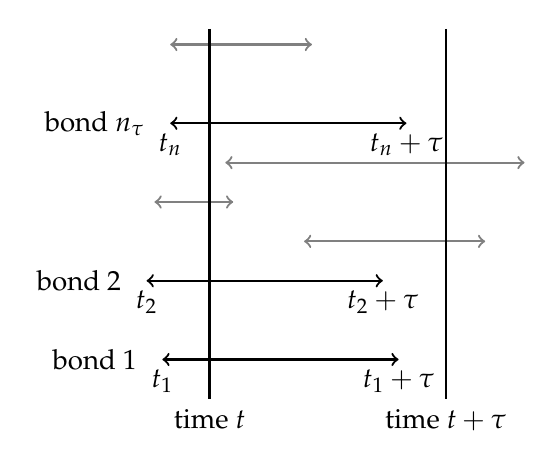
\begin{tikzpicture}[help lines/.style={thin,draw=black!50}]
%%\draw[help lines] (0,0) grid (4,4);
\draw [<->, thick] (0.4,0) node [anchor = north] {$t_1$} -- (3.4,0) node [anchor = north] {$t_1 + \tau$};
\draw (0.2,0) node [anchor = east] {bond $1$};
\draw [<->, thick] (0.2,1) node [anchor = north] {$t_2$} -- (3.2,1) node [anchor = north] {$t_2 + \tau$};
\draw (0,1) node [anchor = east] {bond $2$};
\draw [<->, thick] (0.5,3) node [anchor = north] {$t_n $} -- (3.5,3) node [anchor = north] {$t_n + \tau$};
\draw (0.3,3) node [anchor = east] {bond $n_{\tau}$};
\draw [gray,<->, thick] (1.2,2.5) -- (5.0,2.5);
\draw [gray,<->, thick] (0.3,2) -- (1.3,2);
\draw [gray,<->, thick] (2.2,1.5) -- (4.5,1.5);
\draw [gray,<->, thick] (0.5,4) -- (2.3,4) ;
\draw [thick] (1.0,4.2) -- (1.0,-0.5) node [anchor = north] {time $t$};
\draw [thick] (4.0,4.2) -- (4.0,-0.5) node [anchor = north] {time $t+\tau$};
\end{tikzpicture}
  \caption{\label{fig:P_tc} The H-bonds with lifetime $\tau$ in a certain configuration. 
At time $t$, we assume that there are totally $n_{tot}$ H-bonds can be detected, and $n_{\tau}$ H-bonds are of lifetime $\tau$, therefore,  the fraction of H-bonds that 
have the lifetime $\tau$ in the configuration at time $t$ is $P_{tc}(\tau) =  n_{\tau} /n_{tot}$.
Let $\tau$ take all the values in the interval $[0,\infty]$, we can get the HB lifetime distribution $P_{tc}(t)$.
}
\end{figure}
%\paragraph{Relation Between HB Dynamics and Anisotropy Decay}
%It is interesting to relate the HB kinetics with rotational dynamics (anisotropy decay) of single water molecules.\cite{HX01}
%
\paragraph{Mean First Passage Time Probability Densities}

\paragraph{$k$ and $k'$: Least Squares Fit}
In order to show the effect of water molecule diffusion on the HB dynamics, we can calculate the sum of the functions $c(t)$ and $n(t)$, i.e., $c(t)+n(t)$.
%
\begin{figure}[H]
\centering
\includegraphics [width=0.5\textwidth] {./diagrams/128w_bk_2delta_t_60ps_n}
\setlength{\abovecaptionskip}{0pt}
\caption{\label{fig:128w_bk_2delta_t_60ps_n} 
The time dependence of the population functions $n(t)$ for bulk water, as computed from the ADH (solid line) and AHD (dashed line) criterion of H-bonds.} 
\end{figure}

The probability at time $t$ that a pair of water molecules bonded by H-bonds at the initial moment does not be bonded 
but the distance between their oxygen atoms is still less than $R_{OO}^c$ is 
\begin{eqnarray}
n(t) = \int_0^t dt'k_{in}(t'),
\label{eq:n_from_k_in}
\end{eqnarray}
where $k_{in}(t) = -\langle \dot h(0)[1-h(t)]h^d(t) \rangle/\langle h\rangle$ is the restricted rate function. 
Both Fig. \ref{fig:128w_bk_2delta_t_60ps_n} and Fig.\ref{fig:128w_bk_2delta_t_60ps_n_from_k_in} show the same function $n(t)$. They are calculated from 
$n(t) = \langle h(0)[1-h(t)]h^d(t) \rangle/\langle h\rangle$ and $n(t) = \int_0^t dt'k_{in}(t')$, respectively. 
In each figure, we have drawn the $n(t)$ function corresponding to the two different HB definitions. 
It can be found that neither the calculation method of $n(t)$ nor the definition of HB affects the change trend of $n(t)$, that is, 
as $t$ increases, $n(t)$ increases rapidly from 0, and it reaches the maximum value at $t=10$ ps, and then gradually decreases slowly. [EXPLAIN THE RESULTs]

%
\begin{figure}[H]
\centering
\includegraphics [width=0.5\textwidth] {./diagrams/128w_bk_2delta_t_60ps_n_from_k_in}
\setlength{\abovecaptionskip}{0pt}
\caption{\label{fig:128w_bk_2delta_t_60ps_n_from_k_in} 
The population functions $n(t)$ for bulk water, as computed from the ADH (solid line) and AHD (dashed line) criterion of H-bonds with the definition 
$n(t) = \int_0^t dt'k_{in}(t')$.} 
\end{figure}
Khaliullin and K\"uhne have studied the H-bonding kinetics of pure water using AIMD simulations. [\cite{Khaliullin2013}]
Based on the concepts of $h(t)$, $h^{(d)}(t)$, $n(t)$ and $k(t)$, they have used the simulation data 
obtained by the AIMD simulation method to obtain the ratio $k/k'$ in the bulk water, and then the lifetime and relaxation time 
of the HB.  Here, we also use the AIMD simulation method to study the HB dynamics at the interface of LiI, NaI, and KI aqueous 
solutions. We can obtain the optimal solution range of $k$ and $k'$ from the relationship 
between the reactive flux and the HB population correlation function $c(t)$ and $n(t)$, and the parameters $k$ and $k'$, i.e.,
\begin{eqnarray}
  k(t) = kc(t)-k'n(t).
\label{eq:fitting_k_rates}
\end{eqnarray}
%
%[Answer Q3]
We can find the optimal value of the parameters, $k$ and $k'$, 
by a least squares fit of the calculated data $k(t)$, $c(t)$ and $n(t)$ beyond the transition phase.  
%In order to study the HB dynamics after the transition phase, which is roughly at 0.1 ps (see Fig.\thinspace\ref{fig:121}) and lasts for hundreds of picoseconds. 
For water/vpaor interfaces of neat water and the aqueous solution interfaces, 
the optimal $k$ and $k'$ given by these results have been listed in Table \ref{tab:k_k_prime_pure_and_solutions}. 
These values are comparable in magnitude to those obtained by Ref.\thinspace[{\cite{Khaliullin2013}}] 
% 
\begin{table}[htbp]
\centering
\caption{\label{tab:k_k_prime_pure_and_solutions} 
    The $k$ and $k'$ for the water/vapor interface of the aqueous solution interfaces.} 
\begin{tabular}{cccc}
 Criterion & $k$ (ps$^{-1}$) & $k'$ (ps$^{-1}$) & $\tau_{\text{R}}$ (ps) \\
\hline
  ADH & 0.12 & 0.03 & 8.35 \\
  ADH(from $k_{in}$) & 0.12  & 0.04 & 8.35 \\
  AHD & 0.14 & 0.07 & 14.5 \\
  AHD(from $k_{in}$) & 0.12  & 0.04 & 8.35 \\
\end{tabular}
\end{table}

\section{Water-water Pair Based Hydrogen Bond Dynamics}
The method described in this paragraph is used more in the literature. 
The basis is the population operator $h(t)$ of the HB formed between two water molecules. 
We use the correlation function \CHB to describe the relaxation of H-bonds between two water molecules: [\cite{Luzar1994,AL96,AC00}]
\begin{eqnarray}
C_{\text{HB}}(t)=\langle h(0)h(t) \rangle/\langle h\rangle
\label{eq:C_HB}.
\end{eqnarray}
Similarly, with the aid of the ergodic principle, the ensemble average $\langle \cdots\rangle$ is implemented by time average.
The $\langle h\rangle$ is the probability that a pair of randomly chosen water molecules in the system is
H-bonded at any time $t$. 

The function \CHB is interpreted as the probability that the HB between a certain pair of water molecules is intact at time  $t$, 
if the pair of water molecules are H-bonded at time zero. 
In a large system that consist of many water molecules, the probability that a specific pair of water molecules are H-bonded is extremely small. 
Therefore, the \CHB relaxes to zero, when $t$ is large enough. 
The \CHB measures correlation in $h(t)$ independent of any possible bond breaking events. 
It is one of the intermittent HB correlation functions, introduced by Rapaport, [\cite{DCR83}] 
and can be studied by a continuous function, probability densities.
From the \CHB, the HB relaxation time is computed as [\cite{Lee2007}]


Fig.\ref{fig:128w_bk_2delta_t_60ps_water_pair_c_ns40} shows the correlation function $C_{HB}(t)$ defined by $C_{HB}(t) = \langle h(0)h(t)\rangle/\langle h \rangle$ for bulk water over time. The result is calculated by DFTMD simulation, and the temperature is 300 K. 
\begin{figure}[H]
\centering
\includegraphics [width=0.5\textwidth] {./diagrams/128w_bk_2delta_t_60ps_water_pair_c_ns40}
\setlength{\abovecaptionskip}{0pt}
\caption{\label{fig:128w_bk_2delta_t_60ps_water_pair_c_ns40} 
The correlation functions $C_{HB}(t)$ for bulk water, based on water-water pair hydrogen bond population operator $h(t)$, as computed from the ADH (solid line) and AHD (dashed line) criterion of H-bonds. [DESCRIBE THE FIGURE][COMPARE THE RESULTs TO hbond-based CORRELATION FUNCTION]} 
\end{figure}


\section{Rotational Anisotropy Decay of Water at the Interface of Alkali-Iodine Solutions}\label{CHAPETR_AD}
Using the transition dipole auto-correlation function, 
we determined the rotational anisotropy decay and therefore the OH-stretch relaxation at water/vapor interface of alkali iodide solutions.
%The effects of ion environment on structure and dynamics of water are obtained by comparing the second-order Legendre polynomial, i.e.,  $P_2(x)=\frac{1}{2}(3x^2-1)$,  orientational correlation function of the transition dipole.
The anisotropy decay can be determined from experimental signal in two different polarization configurations---parallel and perpendicular polarizations, by 
\begin{equation}
        R(t)=\frac{S_{\parallel}(t)-S_{\perp}(t)}{S_{\parallel}(t)+2S_{\perp}(t)}
\label{eq:ad}
\end{equation}
where $t$ is the time between pump and probe laser pulses.  The anisotropy decay can also be obtained by simulations, and calculated by the third-order response functions $R(t)$. [\cite{Jansen10,Jansen06}]
%
%In the first shell with a radius 3 \A, the entropy difference betweem the \Li shell and \Na shell,
%$\Delta S=k_B\text{ln}\frac{\Omega_\text{Na}}{\Omega_\text{Li}}=k_B\text{ln}\frac{n_\text{Na}/V_\text{Na}}{n_\text{Li}/V_\text{Li}} =k_B\text{ln}1.05$.
%
%\paragraph{Probability Distribution of Ions}
%The probability distribution, shown in Fig.~\ref{fig: prob_124_LiI_Sans_double_axis}, of the ions in the water/vapor interface of LiI and NaI solutions with repect to the depth of the ions in the solutions 
%indicates that the \I ions prefer to staying at the topmost layer of surface of solutions.
%(molar concentration: 0.9 M, temperature: 330 K) 
%It shows that \I ions tend to the surface of the solutions, while \Na and \Li tend to stay in the bulk. This result is consistent with the calculations from Ishiyama and Morita\cite{TI07,TI14}.
The orientational anisotropy $C_2(t)$ is given by the rotational time-correlation function 
\begin{equation}
C_2(t)=\langle P_2(\hat{u}(0)\cdot\hat{u}(t)) \rangle,
\label{eq:tcf2}
\end{equation}
where $\hat{u}(t)$ is the time dependent unit vector of the transition dipole, $P_2(x)$ is the second Legendre polynomial, and $\langle \rangle$ indicate 
equilibrium ensemble average. [\cite{Corcelli05,LinYS2010}] %\cite{2010Lin} % angular brackets

The anisotropy decay $C_2(t)$ for the water/vapor interface of LiI solution is shown in Fig.\space\ref{fig:c2_2LiI_16_inset}.
This function decays faster than that of neat water, indicating that H-bonds
at the interfaces of alkali-iodine solutions reorient faster than in neat water. The inset shows the first 0.4 ps of $C_2(t)$, from which we see a 
quick change during the first $\sim 0.1$ ps primarily due to librations.
%
\begin{figure}[h]
\centering
\includegraphics [width=0.6\textwidth] {./diagrams/c2_2LiI_16_inset} 
\setlength{\abovecaptionskip}{0pt}
  \caption{\label{fig:c2_2LiI_16_inset} The time dependence of the $C_2(t)$ of OH bonds at the water/vapor interfaces of 0.9 M LiI solution and of neat water (dashed line) at 330 K, calculated by DFTMD simulations. The water/vapor interface of neat water is modeled with a slab made of 121 water molecules in a simulation box of size $15.6 \times 15.6 \times 31.0$ \A$^3$.}
\end{figure}
%
We also calculated the $C_2(t)$ for the interface of other alkali-iodine solutions LiI and KI. 
The results of $C_2(t)$ for the water/vapor interfaces of these solutions are shown in Fig.\space\ref{fig:c2_2KI_2NaI_2LiI_16}.
In all the cases $C_2(t)$ decays faster than in neat water, indicating that H-bonds
at the interfaces of the three alkali-iodine solutions are orientated faster than that of neat water.
They show that \I ions can accelerate the dynamics of molecular reorientation of water molecules at interfaces.   

%
\begin{figure}[htbp]
\centering
\includegraphics [width=0.6 \textwidth] {./diagrams/c2_2KI_2NaI_2LiI_16} 
\setlength{\abovecaptionskip}{0pt}
  \caption{\label{fig:c2_2KI_2NaI_2LiI_16} The time dependence of the $C_2(t)$ of OH bonds in water molecules at the water/vapor 
  interface of 0.9 M alkali-iodine solutions and of neat water (dashed line) at 330 K, calculated by DFTMD simulations.}
\end{figure} 

We have obtained non-single-exponential kinetics for the rotation of water molecules both at the surface 
and in bulk water (Appendix \ref{single_exp}).
%This result is true for water molecules bound to ions. 
Therefore, the rotational motion of water molecules are not simply characterized by well-defined rate constants. 
%Then the problem is to understand the kinetics.
Similar non-single-exponential kinetics is also obtained in the HB kinetics
in liquid water [\cite{AL96,Dirama05}] and in the time variation of the average frequency shifts of the 
remaining modes after excitation in hole burning technique [\cite{Rey2002,Moller2004}] and using BLYP functional. [\cite{Bankura2014}]
Luzar and Chandler interpreted 
the non-single-exponential kinetics as the result of an interplay between 
diffusion and HB dynamics. [\cite{AL96}] 
We can understand the non-single-exponential kinetics of rotational 
anisotropy decay by fitting the rotational anisotropy decay by a 
biexponential function.

To obtain the effects of diffusion and HB decay of water molecules
in solutions respectively, we assume that there are two independent 
decays in the process of an anisotropy decay. 
Therefore, the $C_2(t)$ has the form [\cite{TanHS05}]
\begin{equation}
C_2(t)=A_1e^{-\kappa_1 t} +A_2e^{-\kappa_2 t},
\label{eq:tcf3}
\end{equation}
where $A_i$ are constants and $\kappa_i$ are decay rates ($i=1, 2$). 
The time constants and amplitudes of the biexponentials fits for 
the $C_2(t)$ are listed in Table ~\ref{tab:2LiI_c2_biexp} and Table ~\ref{tab:2NaI_c2_biexp}.
The biexponential fit is very close to the calculated $C_2(t)$, which can be seen in Fig.\space\ref{fig:2LiI-124w_c2_fit_5ps_biexp} (compare Fig.\space\ref{fig:2LiI-124w_c2_fit_5_single-exp}).
%
\begin{table}[hbt]
\centering
\caption{\label{tab:2LiI_c2_biexp}%
	Biexponential fitting (5 ps) of the $C_2(t)$ for water molecules in 0.9 M LiI solution.}
%\begin{ruledtabular}
\begin{tabular}{lccccc}
water molecules & $A_1$  & $\kappa_1$ (THz) & $A_2$ & $\kappa_2$ (THz) \\
\hline
I$^-$-shell & 0.44 & 0.25 & 0.39 & 0.26\\
Li$^+$-shell & 0.88 & 0.07 & 0.07 & 8.24\\
bulk & 0.84 & 0.11 & 0.09 & 4.88 \\
surface & 0.73 & 0.27 & 0.22 & 13.47 \\
\end{tabular}
%\end{ruledtabular}
\end{table}
%--

\begin{table}
\centering
  \caption{\label{tab:2NaI_c2_biexp}%
	Biexponential fitting (5 ps) of the $C_2(t)$ for water molecules in 0.9 M NaI solution.}
  \begin{tabular}{lccccc}
  water molecules & $A_1$  & $\kappa_1$ (THz) & $A_2$ & $\kappa_2$ (THz) \\
  \hline
  I$^-$-shell & 0.86 & 0.14 & 0.08 &9.86 \\
  Na$^+$-shell & 0.71 & 0.06 & 0.18 &0.79 \\
  bulk & 0.81 & 0.06 & 0.10 & 1.25 \\
  surface & 0.77 & 0.11 & 0.13 & 2.31 \\
  \end{tabular}
\end{table}
%
%图
\begin{figure}[htbp]
\centering
\includegraphics [width= \textwidth] {./diagrams/2LiI-124w_c2_fit_5_biexp} 
  \caption{\label{fig:2LiI-124w_c2_fit_5ps_biexp} The time dependence of the $C_2(t)$ of OH bonds 
  in water molecules at the water/vapor interface of LiI solution.}
\end{figure} 
%
%[Notes: The 63-water-slab models is listed here as a reference. The number of water molecules is small; The data for KI/vapor and LiI/vapor interfaces come from  KI\_16 and LiI\_16 systems.  
%Water(63) &0.831$\pm(1\times10^{-4})$ &  0.08760 $\pm(2\times 10^{-5})$&0.100$\pm(2\times10^{-4})$ & 1.029 $\pm(4\times10^{-3})$  \\ ]
%
%\begin{figure}[htbp]
%\centering
%\includegraphics [width=0.4 \textwidth] {./diagrams/c2_121-pure_2KI_2LiI_16_inset_fit_biexp} 
%\setlength{\abovecaptionskip}{10pt}
%\caption{\label{fig:c2_121-pure_2KI_2LiI_16_inset_fit_biexp} The fitted and calculated anisotropy decay of OH bonds in water molecules in LiI solution/vapor interface (red), LiI solution/vapor interface (blue) and neat water/vapor interface (black). The corresponding fitted functions are denoted by dashed lines. The concentration of LiI and KI solution is 0.9 M.}
%\end{figure} 

Then we considered the effect of ion species in solutions on the anisotropy decay of water molecules.
From Table \ref{tab:2LiI_c2_biexp} and Table \ref{tab:2NaI_c2_biexp}, we find that 
for both LiI and NaI solutions, there are two decay processes in the dynamics --- amplitude $\sim 1$,
decay constant $\sim$ 0.1 THz, and for the other describe the initial fast decay 
of the anisotropy, with amplitude $\sim 0.1$, decay constant $\sim$ (1--10) THz, 
due to the inertial-librational motion preceding the orientational diffusion.
That is, two decay processes exist in the dynamics of water molecules 
at the water/vapor interfaces of alkali-iodine solutions. 
%The one describe the initial fast decay of the anisotropy, 
%with amplitude $\sim$ 0.1, decay constant $\sim$ (1--10) THz,
%results from the inertial-librational motion preceding the orientational diffusion.
%
\begin{table}[H]
\centering
\caption{\label{tab:fitting_c2_for_each_type_of_water}%
  Biexponentially fitting (2 ps) of the $C_2(t)$ for different types of water molecules at the water/vapor interface of LiI solutions.}
\begin{tabular}{lccccc}
water molecules & $A_1$  & $\kappa_1$ (THz) & $A_2$ & $\kappa_2$ (THz) \\
\hline
$DDAA$ & 0.85 & 0.25   & 0.10 & 16.0\\
$DD'AA$ & 0.89 & 0.14  & 0.06 & 14.1 \\
$D'AA$ & 0.38 & 0.99 & 0.38 & 0.99 \\
\end{tabular}
\end{table}
%
\begin{table}[H] %[!hbtp]
\centering
\caption{\label{tab:table_CoordNo}%
The coordination number of the atoms in LiI (NaI) solutions.}
\begin{tabular}{lccc}
name & radius of the first shell (\AA) & coordination number \\
\hline
$n_\text{I-H}(\text{LiI})$ & 3.3 & 5.5 \\
$n_\text{I-H}(\text{NaI)}$ & 3.3 & 5.1 \\
$n_\text{I-O}(\text{LiI)}$ & 4.3 & 5.8 \\
$n_\text{I-O}(\text{NaI)}$ & 4.3 & 6.0 \\
$n_\text{Li-O}(\text{LiI)}$ & 3.0 & 4.0 \\
$n_\text{Na-O}(\text{NaI)}$ & 3.5 & 6.0 
\end{tabular}
\end{table}

\section{I$^-$--Water Hydrogen Bonds in Aqueous Solutions}
In the case of water--water hydrogen bonds, the critical distance of $R_c^{OO}=3.5$ \AA are the position of the first minimum of the oxygen--oxygen RDF.
For the anion--oxygen hydrogen bonds, we can use the similar criteria. The cutoff values for $X$--oxygen distance are obtained from the positions of the first
minimum of the $X$--oxygen RDF, i.e., $R_c^{XO}=4.1$, 3.7 \A, for $X$ = I$^-$ and nitrate O. We have still used $30^{\circ}$ for the anglar cutoff.\cite{Chowdhuri2006}
\begin{figure}[htbp]
\centering
\includegraphics [width=0.6 \textwidth] {./diagrams/gdr_127_LiNO3} 
\setlength{\abovecaptionskip}{0pt}
  \caption{\label{fig:gdr_127_LiNO3} (a)Li--water O, Li--water H RDFs; (b) Nitrate O--water O, nitrate O-water H RDFs for LiNO$_3$ solutions at 300 K. The RDFs were computed from DFTMD.}
\end{figure}
The function $C_{HB}$ of I$^-$--water and water--water hydrogen bonds describes the structural relaxation of these H- bonds. The results of the $C_{HB}(t)$ are shown in Figure \ref{fig:X-O_c_lii}. 
\begin{figure}[htbp]
\centering
\includegraphics [width=0.6 \textwidth] {./diagrams/X-O_c_lii} 
\setlength{\abovecaptionskip}{0pt}
  \caption{\label{fig:X-O_c_lii} Time dependence of the intermittent correlation functions of I$^-$--water (I$^-$--W) and water--water hydrogen bonds at 300 K.}
\end{figure}
The results of the continuous correlation functions for both definitions (ADH and AHD criterions) for the H-bonds are shown in Figure \ref{fig:wat-wat_s_lii} 
for I$^-$--water hydrogen bonds. The results of water--water hydrogen bonds are also included for comparison in both Figure \ref{fig:wat-wat_s_lii} (a) and (b).
\begin{figure}[htbp]
\centering
\includegraphics [width=0.6 \textwidth] {./diagrams/wat-wat_s_lii} 
\setlength{\abovecaptionskip}{0pt}
  \caption{\label{fig:wat-wat_s_lii} Time dependence of the continuous correlation functions of I$^-$--water (I$^-$--W) and water--water hydrogen bonds at 300 K.}
\end{figure}
For both definitions for the H-bonds, it is found that the I$^-$--water hydrogen bonds show faster dynamics than water--water hydrogen bonds. 
(consistent to the previous MD results.) Therefore, the time scales of the relaxation of these H-bonds can be obtained for both definitions. 
In Table \ref{tab:properties_anion-water_hbs}, we have included the average lifetimes $\langle\tau_{a}\rangle$, which can be cumputed from Eq.\ref{eq:calculate_hb_lifetime}, 
for both water--water and I$^-$--water hydrogen bonds. We performing the fitting in the time region 0.2 ps < $t$ < 12 ps to calculate the forward and backward rate constants
for HB breaking.
%
\begin{table}[htbp]
\centering
\caption{\label{tab:k_k_prime_pure_and_solutions} 
    The Dynamical properties of anion--water and water--water hydrogen bonds at 300 K. Data are from DFTMD for the aqueous solutions. The values are expressed in ps.} 
\begin{tabular}{ccccc}
\label{tab:properties_anion-water_hbs}
 Quantity & Criterion & W--W & I$^-$--W & NO$_3^-$--W  \\
\hline
  $\langle\tau_a\rangle$  & ADH & 190.3 & 0.10 & 4.35 \\
  $\langle\tau_a\rangle$ & AHD & 186.8  & 0.11 & 7.91 \\
  $1/k$ & ADH & 9.82 & 2.80 & 4.15 \\
  $1/k$ & AHD & 8.97 & 2.40 & 6.02\\
\end{tabular}
%
% Data from: LiI solution:  gang@XPS /home/gang/Github/water_pair_HB_dynamics/src/least_square_fit
% Data from: LiNO3 solution:  /home/gang/Github/water_pair_HB_dynamics/src/least_square_fit/LiNO3 
\end{table}
\begin{figure}[htbp]
\centering
\includegraphics [width=0.6 \textwidth] {./diagrams/I--wat_n_lii} 
\setlength{\abovecaptionskip}{0pt}
  \caption{\label{fig:I--wat_n_lii} Time dependence of the correlation functions $n_{HB}(t)$ of I$^-$--water (I$^-$--W) and water--water hydrogen bonds at 300 K.}
\end{figure}

 
\chapter{Hydrogen Bond Dynamics of Water/Vapor Interfaces }\label{CHAPTER_HB_WATER}
%The influence of ions propensity for the aqueous surface on the water's HB network are also of special interest to the atmospheric chemistry community.
In this chapter, we explore the effects of nitrate ions, iodide ions and alkali metal cations 
on the HB dynamics at the water/vapor interface of alkali nitrate solutions and alkali
iodine solutions, by DFTMD 
and we provide a microscopic interpretation of recent experimental results. \cite{HuaWei2014}

\section{Effects of ions on HBD}
The configuration criterion above allows us to define a variable $h[r(t)] = h(t)$, HB population. 
The $h(t)$ has a value 1 when the particular tagged pair of molecules are bonded, and 0 otherwise. 
%=================
% added 2020-5-27: to show that h(t) is actually the fluctuation of itself (\delta h).
We know that the instantaneous fluctuation or deviation in a dynamical variable $A(t)$ from its time-independent equilibrium average $\langle A\rangle$ , 
is defined by [\cite{DC87}] 
$$
\delta A = A(t) - \langle A\rangle.
$$
For the $h(t)$, since the probability that a specific pair of molecules is bonded in a large system is extremely small, i.e., 
the time average of $h$ is zero, or  
$\langle h \rangle = 0$,
then 
$$
\delta h(t) = h(t).
$$
Therefore, the $h(t)$ describe the instantaneous fluctuation $\delta h(t)$  of the HB population.  
%The behaviour of $r_{OO}(t)$  is depicted in Fig.\ref{fig:Ex30ps_hb}(a). We find that in the equilibrium system, $r_{OO}(t)$ looks chaotic.
%=================

While the equilibrium average of the $\delta h(t)$ is zero, but we can obtain useful information by considering the equilibrium 
correlations between fluctuations at different times. The correlation between the $\delta h(t)$ and the $\delta h(0)$ can be written as 
$$
\langle \delta h(0) \delta h(t)\rangle = \langle h(0)h(t)\rangle-\langle h \rangle^2 = \langle h(0)h(t)\rangle,
$$
where the averaging $\langle\cdots\rangle$ is to be performed over the ensemble of initial conditions $(r^N, p^N)$.


\FloatBarrier
\section{Environment Effects on Hydrogen Bond Dynamics}
For the water/vapor interface of neat water, we focus on the reactive flux $k(t)$, 
which had been used in the study of HB dynamics of liquid water. [\cite{AL96,Khaliullin2013}]
The $k(t)$ calculated from the positional trajectory of water molecules in DFTMD simulations, is reported in Fig.\space\ref{fig:121}. 
In the case of water/vapor interface, the $k(t)$ quickly changes from its initial value on a time scale of less than 0.2 ps 
(see the inset of Fig.\space\ref{fig:121}). 
Beyond this transient period, the $k(t)$ decays to zero monotonically, and the slop of the $\ln{k(t)}$ increases monotonically with $t$ (see Fig.\space\ref{fig:121_log_rf}). 
These two properties were also found for bulk water using the SPC water model by Luzar and Chandler. [\cite{AL96}] 
This log-log plot of the $k(t)$ shows that, as in the case of liquid water, this decay behaviour does not coincide with a power-law decay for water/vapor interface of neat water.
This result is also the same as that of the classical molecular simulation of pure water. [\cite{AL96b,Luzar1996}]
%
\begin{figure}[htpb]
\centering
\includegraphics [width=0.5\textwidth] {./diagrams/121}
\setlength{\abovecaptionskip}{0pt}
  \caption{\label{fig:121}The time dependence of the $k(t)$ for the water/vapor interface of neat water, calculated by DFTMD simulations.
  The inset shows the log-log plot of the $k(t)$.}
\end{figure}
%

We focus on the value of the $k(t)$ when $t$ is sufficiently large ($t \in [1, 10]$ ps). 
The $k(t)$ in Fig. \ref{fig:hbrf_4pl} are calculated by the interface 
under the same condition. The difference is that Fig.\thinspace\ref{fig:hbrf_4pl} (a) is the result of the interface of pure water,
and Fig. \ref{fig:hbrf_4pl} (b), (c) and (d) are the result of the interface of the LiI, NaI and KI solutions, respectively. 
%
\begin{figure}[htpb]
\centering
\includegraphics [width=0.5\textwidth] {./diagrams/121_pure_ns20_log_rf}
\setlength{\abovecaptionskip}{0pt}
  \caption{\label{fig:121_log_rf}The time dependence of the $\ln{k(t)}$ for the water/vapor interface of neat water, calculated by DFTMD simulations.}
\end{figure}
\begin{figure}[H]
\centering
\includegraphics [width=1.0\textwidth] {./diagrams/hbrf_4pl}
\setlength{\abovecaptionskip}{0pt}
  \caption{\label{fig:hbrf_4pl}The time dependence of the $k(t)$ for the water/vapor interfaces 
  with different thickness $d$ ($d$= 2, 3, 4 and 5 \AA) of four interface models calculated by DFTMD simulations. 
  The value of $h(t)$ is calculated every 0.1 ps. 
  (a): neat water; (b): 0.9 M LiI solution; (c): 0.9 M NaI solution; (d): 0.9 M KI solution.} 
\end{figure} 
%
\begin{table}[htbp]
\centering
\caption{\label{tab:hbrf_neat} 
   The average value of $k(t)$ (unit: ps$^{-1}$) over different time periods of 2 ps for layers of the water/vapor interface of neat water.  
   $\overline{k(t)}_{\Delta t}$ denotes the average value of $k(t)$ over the time period $\Delta t$.} 
\begin{tabular}{cccc}
  Thickness($d$) & $\overline{k(t)}_{\text{2--4 ps}}$ & $\overline{k(t)}_{\text{4--6 ps}}$ & $\overline{k(t)}_{\text{6--8 ps}}$\\
\hline
  2\AA & 0.027 & 0.019 & 0.019\\
  3\AA & 0.028 & 0.021 & 0.020 \\
  4\AA & 0.031 & 0.025 & 0.022 \\
  5\AA & 0.028 & 0.019 & 0.014 
\end{tabular}
\end{table}
%
%For the water/vapor interface of alkali-iodine solutions, the $k(t)$ is also calculated.  The result for the interface of 0.9 M LiI solution is shown in Fig.\thinspace\ref{fig:hbrf_4pl} (b). The log-log plot of $k(t)$ is not a straight line, indicating that, for water/vapor interface of the LiI solution, this decay does not coincide with a power-law decay, neither.


%{As can be seen from Fig. \ref{fig:hbrf_4pl}, the fluctuations of the $k (t)$ for $d = 2$ \AA (blue solid line) are significantly larger 
%than that of other cases with larger $d$. 
%This phenomenon is due to the relatively small number of water molecules in the thin layer 
%and the insufficient sampling, resulting in large fluctuations in $k(t)$.
%For these four models, as the thickness $d$ of the interface increases, the $k(t)$ gradually converges to a function with smaller fluctuations.
%%
%This conclusion is consistent with the two conclusions we obtained earlier (see Section \ref{sfg_alkali_iodide_interface}): 
%(1) \I is a strong structure-breaking anion; %[\cite{Trevani2000}] 
%(2) compared to pure water, the OH stretching peak at the interface of a solution containing iodide ions will blue shift. [\cite{Tongraar2010}] 
%Comparing these black solid curves, we can see that the interface of the solution containing ions has lower $k(t)$.
%In other words, compared to the pure water interface, 
%the ratio of H-bonds that were initially bonded at the solution interface and broken at time $t$ is lower.
%Because the effect of iodide ions is to increase the $k(t)$ of the interface, the decrease of $k (t)$ of the interface with a larger thickness
%may only be due to the contribution of cations located under the first layer of water molecules at the interface. 
%Therefore, although the iodide ion increases the HB rupture rate at the top layer of the interface, 
%in general, the HB rupture rate of the entire solution interface is reduced due to the presence of cations under the first layer of water molecules. 
%To verify this conclusion, we calculated the $k(t)$ at the interface of NaI (Fig. \ref{fig:hbrf_4pl} (c)) and KI (Fig. \ref{fig:hbrf_4pl} (d)) aqueous solution. 
%The results for both interface systems support our conclusions above.
%}
%\stkout{ What is the differences between bulk and interface? 
%Let us examine the difference in the $k(t)$ between interface water and bulk water. 
%No matter from pure water (Fig. \ref{fig:hbrf_4pl} (a)) 
%or solution (Fig. \ref{fig:hbrf_4pl} (b), (c) or (d)), we find that when the interface thickness is thin, the fluctuation of $k(t)$ is larger.
%Because the thinner the interface, the fewer pairs of water molecules that can form hydrogen bonds. 
%In our calculations, the fewer samples are used to average, so the fluctuation of $k (t)$ is greater. 
%We can find that at the interface of pure water, when $t> 0.2$ ps, the $k(t)$ value of the interface with different thickness is almost equal 
%at any time period $\Delta t$. For example, $\Delta t$ is selected as $\sim$ 2 ps, 
%and its average value is shown in Table \ref{tab:hbrf_neat}. In each time period of 2 ps, the values of $k(t)$ for different layers are approximately equal
%($\pm 0.004$ ps$^{-1}$). Therefore, as far as the nature of HB reactive flux is concerned, the difference between interface and bulk phase of neat water is not obvious. 
%}

In order to show the effect of water molecule diffusion on the HB dynamics, we can calculate the sum of the functions $c(t)$ and $n(t)$, i.e., $c(t)+n(t)$.
%Here, we take the LiI solution as an example.
Fig.\space\ref{fig:124_2LiI_ns20_c_plus_n} shows the time dependence of the correlation functions $c(t)$, $n(t)$ and $c(t)+n(t)$ of the interface of 
the LiI solution at a concentration of 0.9 M in the AIMD simulation.
As can be seen, although the change in the total population, $c(t)+n(t)$, is very small in the range of 0--10 ps, it is not a constant.
Therefore, the $n(t)$ relaxes not only by conversion back to HB \emph{on} state, 
but is also depleted due to the diffusion process. We can estimate the time scale of water molecule diffusion at the interface of the aqueous solution by $c(t)+n(t) = 1/e$, 
which is much larger than 10 ps. Therefore, when we analyze the HB dynamics of the solution interfaces, we do not consider the effect of water molecule diffusion.
%
\begin{figure}[H]
\centering
\includegraphics [width=0.5\textwidth] {./diagrams/124_2LiI_ns20_c_plus_n}
\setlength{\abovecaptionskip}{0pt}
\caption{\label{fig:124_2LiI_ns20_c_plus_n} 
The time dependence of the functions $c(t)$, $n(t)$ and $c(t)+n(t)$, where $c(t)$ represents the $C_{\text{HB}}(t)$, 
for the interfaces of 0.9 M LiI solution.} 
\end{figure}
%
\begin{figure}[H]
\centering
\includegraphics [width=0.5\textwidth] {./diagrams/128w_bk_2delta_t_60ps_n}
\setlength{\abovecaptionskip}{0pt}
\caption{\label{fig:128w_bk_2delta_t_60ps_n} 
The time dependence of the population functions $n(t)$ for bulk water, as computed from the ADH (solid line) and AHD (dashed line) criterion of H-bonds.} 
\end{figure}

Khaliullin and K\"uhne have studied the H-bonding kinetics of pure water using AIMD simulations. [\cite{Khaliullin2013}]
Based on the concepts of $h(t)$, $h^{(d)}(t)$, $n(t)$ and $k(t)$, they have used the simulation data 
obtained by the AIMD simulation method to obtain the ratio $k/k'$ in the bulk water, and then the lifetime and relaxation time 
of the HB.  Here, we also use the AIMD simulation method to study the HB dynamics at the interface of LiI, NaI, and KI aqueous 
solutions. We use the least squares fitting method to obtain the optimal solution range of $k$ and $k'$ from the relationship 
between the reactive flux and the HB population correlation function $c(t)$ and $n(t)$, and the parameters $k$ and $k'$, i.e.,
\begin{eqnarray}
  k(t) = kc(t)-k'n(t).
\label{eq:fitting_k_rates}
\end{eqnarray}
%
%[Answer Q3]
We can find the optimal value of the parameters, $k$ and $k'$, 
by minimizing the function $\Delta(k,k') = \int_{t_1}^{t_2} \big|\ln[kc(t)-k'n(t)] - \ln[k(t)]\big|dt$. 
In order to study the HB dynamics after the transition phase, which is roughly at 0.1 ps (see Fig.\thinspace\ref{fig:121}) and lasts for hundreds of picoseconds, 
we set $t_1 = 1$ ps and $t_2 = 10$ ps in the fitting.
For water/vpaor interfaces of neat water and the aqueous solution interfaces, the fitting results we obtained are plotted in 
Fig.\thinspace\ref{fig:121_pure_ns20_fit_map}--\ref{fig:124_2KI_ns20_fit_map}, 
and the optimal values of $k$ and $k'$ given by these results have been listed in Table \ref{tab:k_k_prime_pure_and_solutions}. 
These values are comparable in magnitude to those obtained by Ref.\thinspace[{\cite{Khaliullin2013}}] 
% pure water fitting map
\begin{figure}[htbp]
\centering
\includegraphics [width=0.5\textwidth] {./diagrams/121_pure_ns20_fit_map}
\setlength{\abovecaptionskip}{0pt}
\caption{\label{fig:121_pure_ns20_fit_map} 
The contour plot of the function $\Delta(k,k')$ for the interfaces of neat water.} 
\end{figure}
% 
\begin{figure}[htbp]
\centering
\includegraphics [width=0.5\textwidth] {./diagrams/124_2LiI_ns20_fit_map}
\setlength{\abovecaptionskip}{0pt}
\caption{\label{fig:124_2LiI_ns20_fit_map} 
The contour plot of the function $\Delta(k,k')$ for the interfaces of 0.9 M LiI solution.} 
\end{figure}
%
\begin{figure}[htbp]
\centering
\includegraphics [width=0.5\textwidth] {./diagrams/124_2NaI_ns20_fit_map}
\setlength{\abovecaptionskip}{0pt}
\caption{\label{fig:124_2NaI_ns20_fit_map}
The contour plot of the function $\Delta(k,k')$ for the interfaces of 0.9 M NaI solution.} 
\end{figure}
%
\begin{figure}[htbp]
\centering
\includegraphics [width=0.5\textwidth] {./diagrams/124_2KI_ns20_fit_map}
\setlength{\abovecaptionskip}{0pt}
\caption{\label{fig:124_2KI_ns20_fit_map}
The contour plot of the function $\Delta(k,k')$ for the interfaces of 0.9 M KI solution.} 
\end{figure}
%
\begin{table}[htbp]
\centering
\caption{\label{tab:k_k_prime_pure_and_solutions} 
    The $k$ and $k'$ for the water/vapor interface of the aqueous solution interfaces.} 
\begin{tabular}{cccc}
 Interface & $k$ (ps$^{-1}$) & $k'$ (ps$^{-1}$) & $\tau_{\text{R}}$ (ps) \\
\hline
  Neat Water & 0.10 $\pm$ 0.02 & 0.20 $\pm$ 0.02 & 11.50 \\
  LiI & 0.10 $\pm$ 0.04 & 0.30 $\pm$ 0.05 & 5.33 \\
  NaI & 0.20 $\pm$ 0.10 & 0.30 $\pm$ 0.05 & 5.77 \\
  KI  & 0.10 $\pm$ 0.04 & 0.40 $\pm$ 0.10 & 6.96 
\end{tabular}
\end{table}
It can be seen from Table \ref{tab:k_k_prime_pure_and_solutions} that the HB breaking reaction rate ($k$) at the interface of pure water is basically equivalent to 
that at the solution interface, but the HB reforming rate ($k'$) is smaller than that at the solution interface by 30\% to 50\%.
Correspondingly, we can find the HB relaxation times of the three solution interfaces are: $\tau=\frac{1}{k+k'} \sim $2.0--2.5 ps. 
For pure water interface, the relaxation time is $\tau \sim $ 3.3 ps. 
Our conclusion is that the difference between the relaxation time of H-bonds at the interface of solutions such as LiI, NaI, KI 
and the interface of pure water is mainly due to the difference in the reforming rate $k'$ of H-bonds caused by the presence of ions,
rather than the difference in the breaking rate $k$ of H-bonds.

As for the effect of water/vapor interface on the HB dynamics in alkali-iodine solutions,
we also calculate the survival probability for interfaces with different sizes of thickness. 
The result for the interface of the LiI solution exhibits that H-bonds at water/vapor 
interface decay faster than that in bulk water.
The result for the logarithm of \SHB is displayed in Fig.\space\ref{fig:2LiI-124w_S_layers} in Appendix \ref{thickness_interface}, 
in which the thickness of the alkali-iodine solutions can be determined.
Therefore, as the interface thickness increases, the \SHB converges to a curve, 
which characterizes the HB dynamics of bulk solutions. 
In particular, it gives the average continuum HB lifetime in bulk solutions.
\FloatBarrier
\paragraph{Effects of the Ions Concentration}
Effects of ions' concentration on HB dynamics have been studied extensively by Chandra. [\cite{AC00}]
%Pal and coworkers provided details on the structure of water around the micellar surface.\cite{SP05} 
We calculated the \CHB for the water/vapor interfaces of the alkali-iodine solutions, 
and the relaxation time $\tau_{\text{R}}$ for each of them can be determined. 
%\begin{eqnarray}
%    C_{\text{HB}}(\tau_\text{{R}})=1/e. \nonumber
%\label{eq:relaxation_time}
%\end{eqnarray}
Here, the \emph{interface} means \emph{all} the water molecules in each model. 
The $\tau_{\text{R}}$ for the water/vapor interfaces of the LiI (NaI) solutions are displayed in 
Table \ref{tab:tau_hb}. Generally, they are in the range 1--10 ps. 
The values of $\tau_{\text{R}}$ decrease as the concentration of the solutions increases.
\begin{table}[htbp]
\centering
\caption{\label{tab:tau_hb} 
  The relaxation time $\tau_{\text{R}}$ (unit: ps) of the correlation function \CHB  for the water/vapor interface of the LiI (NaI) solutions, calculated by DFTMD simulations.}
\begin{tabular}{ccc}
  concentration  & $\tau_{\text{R}}$ (LiI) & $\tau_{\text{R}}$ (NaI) \\
\hline
  0 & 11.50 & 11.50 \\
  0.9 M & 7.04 & 10.60 \\
  1.8 M & 4.40 & 1.96 
\end{tabular}
\end{table}

The concentration dependence of the HB dynamics can be also found in the \SHB. 
Fig.\space\ref{fig:124_2LiI-2NaI_hbacf_S}(a) gives the \SHB 
for the water/vapor interfaces of 0.9 M and 1.8 M LiI solutions.
The same quantity for NaI solutions is displayed in Fig.\space\ref{fig:124_2LiI-2NaI_hbacf_S}(b).
This result indicates that, for the interface of alkali-iodine solution, the continuum HB lifetime  
decrease as the concentration of LiI (or NaI) solution increase.
\begin{figure}
\centering
\includegraphics [width=1.1\textwidth, center] {./diagrams/124_2LiI-2NaI_hbacf_S} 
\setlength{\abovecaptionskip}{0pt}
  \caption{\label{fig:124_2LiI-2NaI_hbacf_S} The time dependence of the \SHB  of 
  H-bonds at the water/vapor interfaces of (a) LiI and (b) NaI solutions at 330 K.
	The insets show the plots of ln$S_{\text{HB}}(t)$.} 
\end{figure}
%%
\FloatBarrier
\paragraph{Effect of Nitrate ions}
%I simulate the alkali nitrate solution/vapor interface to find how the nitrate affect the structure of the interface.
\begin{figure}[htbp] % or \begin{SCfigure}
\centering
\includegraphics [width=0.6\textwidth] {./diagrams/256_LiNO3_hbacf_sh_no3} %fig.5.10
\setlength{\abovecaptionskip}{0pt}
\caption{\label{fig:256_LiNO3_hbacf_sh_no3} The \SHB of water--water (W--W) and nitrate--water (N--W) H-bonds at the water/vapor
  interface of the \LiN solution. The inset is the plot of ln\SHB. 
  These results are calculated for the temporal resolution $t_t=1$ fs. For the definition of $t_t$, please refer to the Appendix \ref{thickness_interface}. }
\end{figure}
%
%\begin{figure}[H]
%\centering
%\includegraphics [width=0.4\textwidth] {./diagrams/256_LiNO3_hbacf_hh_all_traj_sh_no3}
%\setlength{\abovecaptionskip}{20pt}
%\caption{\label{fig:256_LiNO3_hbacf_hh_all_traj_sh_no3}The functions ln\SHB of water--water H-bonds (black) and Nitrate -water H-bonds (red) in the the \LiN solution-vapor interface at 300 K. The lifetime of H-bonds $\tau_{\text{HB}}$ is calculated by the integration of \SHB over t$\in$(0,$\infty$), which give 0.42  and 0.20 ps, for water--water H-bonds and Nitrate -water H-bonds, respectively.}
%\end{figure}
%The density profile is a indicator of a table interfacial system (see Fig.\space\ref{fig:density_4MPlus_alkali-I}).
%\begin{figure}[htbp]
%\centering
% \includegraphics [width=0.6\textwidth] {./diagrams/density_4MPlus_alkali-I} %fig5.11
%\setlength{\abovecaptionskip}{20pt}
%\caption{\label{fig:density_4MPlus_alkali-I}The density as a function of the slab coordinate \Z. The result is calculated by MD with SPC water model.}
%\end{figure}

As shown in Fig.\space\ref{fig:vdos_LiNO3-256w_w_near_nitrate} in chapter ~\ref{CHAPTER_SFG_Calculation}, 
from the VDOS, the water molecules bound to \nitrate have higher OH stretching frequency (55 cm$^{-1}$ larger) 
than those H-bonded to other water molecules. 
%
Now, the difference between nitrate--water and water--water H-bonds 
can be also analyzed in terms of the survival probability $S_{\text{HB}}(t)$, [\cite{AKS86,JT90,AL96}] 
reported in Fig.\thinspace\ref {fig:256_LiNO3_hbacf_sh_no3}.
The integration of \SHB from 0 to $t_{\max}=5.0$ ps, [\cite{Steinel2004}] gives the relaxation time $\tau_\text{HB}$, which can be interpreted as 
the average HB lifetime. [\cite{SC02}] 
The values of $\tau_{\text{HB}}$ is dependent on a temporal resolution $t_t$, during which the H-bonds that break and reform are treated as intact. [\cite{AL00}] 
%
Here, we choose the temporal resolution as $t_t=1$ fs. 
Then, Fig.\thinspace\ref {fig:256_LiNO3_hbacf_sh_no3} gives $\tau_\text{HB}=0.20$ ps for nitrate--water H-bonds at interfaces, and $\tau_\text{HB}=0.42$ ps for water--water H-bonds.
This result of $\tau_\text{HB}$ is consistent with the experimental result of Kropman and Bakker ($\tau_\text{HB}=0.5\pm0.2$ ps). [\cite{MFK01}]
The smaller value of $\tau_\text{HB}$ for nitrate--water H-bonds implies that the nitrate--water H-bonds are weaker than bonds between water molecules. 
This is also consistent with the VDOS analysis and the blue-shifted frequency of the OH stretching in the nitrate-water HB. 
%[DELETED From both the VDOS and HB dynamics calculations, we conclude that it is the weak HBs between nitrate and water make the higher surface propensity 
%of nitrate anions, and then induce the depletion of SFG intensity at 3200 \cm for the alkali nitrate salty interfaces.]

%Fig. ~\ref{fig:256_LiNO3_hbacf_Nitrate_effect} shows that the nitrate ions accelerate the HB dynamics at the vapor/water interface of alkali nitrate solution.
%\begin{figure}[H]
%\centering 
% \includegraphics [width=0.6\textwidth] {./diagrams/256_LiNO3_hbacf_Nitrate_effect} %fig5.12
%\setlength{\abovecaptionskip}{20pt}
%\caption{\label{fig:256_LiNO3_hbacf_Nitrate_effect}The functions \CHB of bulk water--water H-bonds (W-W (Bulk)) and nitrate--water H-bonds (N-W) 
%at interfaces of alkali nitrate solution  (LiNO$_3$(H$_2$O$_{256}$)  at 300 K. }
%\end{figure} 
%NOT CLEAR, TO EXPLAIN BETTER The HB relaxation time is about $2.5$ ps, which is the same as that
%for nitrate--water H-bonds at interfaces of alkali nitrate solution.
%[NOT CLEAR: For bulk water, the HB relaxation time $\tau$ is $3.7$ ps. The difference between the HB dynamics of H-bonds outside the first shell of \Li and HB dynamics for nitrate--water H-bonds at interfaces
%is not visible from the values of the HB relaxation time. They reflect the difference between HB
%dynamics between bulk water and water/vapor interfaces.]
\FloatBarrier
\paragraph{Effects of Alkali Metal Ions and \I on HB Dynamics}
%\begin{figure}[!ht]
%\centering
%\includegraphics [width=\textwidth] {./diagrams/C_S_HB_124_2LiI-2NaI-2KI} %fig5.15
%\setlength{\abovecaptionskip}{0pt}
%  \caption{\label{fig:C_S_HB_124_2LiI-2NaI-2KI} The time dependence of functions (a) \CHB and (b) \SHB of water--water H-bonds at water/vapor interfaces of 0.9 M alkali-iodine solutions.} 
%\end{figure}
%
\begin{table}[hbtp]
\centering
\caption{\label{tab:tau_hb_alkali_iodine} 
The continuum HB lifetime $\tau_{\text{HB}}$ (unit: ps) in the first hydration shell of I$^-$ ion and of alkali metal ion at the water/vapor interface of 0.9 M LiI (NaI, KI) solution.}
\begin{tabular}{cccc}
  &\I-shell &cation-shell& interface \\
\hline
 LiI & 0.22 & 0.24 & 0.23\\
 NaI & 0.24 & 0.28 & 0.26\\
 KI  & 0.20 & 0.23 & 0.20\\
\end{tabular}
\end{table} 
%Water/Vapor & -&-&
Table \ref{tab:tau_hb_alkali_iodine} lists the continuum HB lifetime in the first hydration shell of I$^-$ ion and of alkali metal ion
at the  interfaces of the three alkali-iodine solutions. It shows that, for all three alkali-iodine solutions, the continuum HB lifetime $\tau_{\text{HB}}$ in the 
solvation shell of alkali metal (iodine) ions is larger (smaller) than 
that of H-bonds at the water/vapor interfaces of the same solutions, 
respectively. For LiI solution, the water molecules bound to the cation ion
\Li, on average, have a continuum HB lifetime $\tau_{\text{HB}} \sim 0.24$ ps. This
 continuum HB lifetime is longer than that of molecules bound to \I or at the interface of the LiI solution. 
%
\begin{figure}[H]
\centering
\includegraphics [width=\textwidth] {./diagrams/hbacf_C_sh2_2p}
\setlength{\abovecaptionskip}{0pt}
\caption{\label{fig:hbacf_C_sh2_2p}The \CHB of water--water H-bonds in the ion solvation shell 
  of (a) cations and (b) I$^-$ at the interfaces of 0.9 M LiI, NaI and KI solutions, respectively.
  The dashed line shows \CHB for the interface (the thickness $d = 8$ \A) of the LiI solution.  
  This interface contains H-bonds between water molecules similar to those in pure bulk water, that is,
  water molecules participating in these H-bonds are not in the solvation shell of ions.} 
\end{figure}
%Fecko and co-workers' study of liquid D$_2$O by IR spectroscopy reveals that the vibrational dynamics observed are dominated by underdamped displacement of the hydrogen-bond coordinate at very short times ( less than 200 fs).\cite{CJF03,CJF05} 
Fig.\space\ref{fig:hbacf_C_sh2_2p} (a) and (b) show that the \CHB of H-bonds within the alkali cations and \I decay faster than those in bulk water and at the surface of LiI solution.
From Fig.\space\ref{fig:hbacf_C_sh2_2p} (b), we find that, for all three alkali-iodine solutions, the \CHB for hydration shell water molecules of \I decays faster than that for molecules at the water/vapor interface.
%The simulation produces similar result as Omta and coworker's experiments of femtosecond pump-probe spectroscopy, which demonstrate that anions ( $\text{SO}^{2-}_4$, $\text{ClO}^-_4$, etc) have no influence on the dynamics of bulk water, even at high concentration up to 6 M.\cite{AWO03} 
%Here, we find that the cations \Li and \Na does not alter the H-bonding network outside the first hydration shell of cations. It is concluded that no long-range structural-changing effects for alkali metal cations.
The radii of hydration shells are 5.0 \AA for \li, 5.38 \AA for \na,
5.70 \AA for \pot, and 6.0 \AA for \I ions, which are obtained from the RDFs.
The RDFs $g_{\text{ion-O}}$ (ion=\li, \na) for the interfaces 
of LiI (NaI) solutions are shown in Fig.\space\ref{fig:124_2NaI-2LiI_gdr_Li-O_Na-O_1501}(a),
and the coordination numbers are in Fig.\space\ref{fig:124_2NaI-2LiI_gdr_Li-O_Na-O_1501}(b).
\begin{figure}[H]
\centering
\includegraphics [width=0.5 \textwidth]{./diagrams/124_2NaI-2LiI_gdr_Li-O_Na-O_1501}%fig.6.1 
\setlength{\abovecaptionskip}{0pt}
\caption{\label{fig:124_2NaI-2LiI_gdr_Li-O_Na-O_1501}
  (a) The RDF $g_{\text{ion-O}}(r)$(ion=\li, \na) and (b) the coordination number of \Li (\na) ions at the interfaces of LiI (NaI) solution. 
	For \Na, the coordination number $n_\text{Na}$=5; while for \Li, $n_\text{Li}$=4.} 
\end{figure} % There is a first shell exist for both \Li and \Na cations.
%\section{Hydrogen Bond Dynamics by Classical Molecular Dynamics Simulations}
%\begin{figure}[H]
%\centering
% \includegraphics [width=0.5\textwidth] {./diagrams/4MPlus-alkali-I_hbacf_C1603}
%\setlength{\abovecaptionskip}{20pt}
%\caption{\label{fig:4MPlus-alkali-I_hbacf_C1603}The function \CHB of water--water H-bonds at interfaces with different alkali metal ions in 4.0 M water solution at 300 K.}
%\end{figure}
%The HB dynamics obtained from classical MD simulations can not catch the fast HB relaxation, and it give a totally different HB dynamics for the water molecules in these alkali halide solution/vapor interfaces.

\section{HBD in Interfaces of Other Alkali Nitrate Solutions}
The probability distribution of O and H atoms in the model of LiNO3 interface is showed in Fig. \ref{fig:prob_wat--ln_itp}. In this paragraph, we study the HBD of the LiNO$_3$ interface.
\begin{figure}[h!]
\centering
\includegraphics [width=0.6 \textwidth] {./diagrams/prob_wat--ln_itp}
\setlength{\abovecaptionskip}{0pt}
\caption{\label{fig:prob_wat--ln_itp} The probability distributions $P(z)$, along the normal direction,
  of O and H atoms in LiNO$_3$ solution-air interface, through the trajectory of 20 ps.
Computational details: The simulated interfacial system consisted of 127 water molecules and a Li$^+$-Nitrate pair in a periodic
box of size $15.7787 \times 15.7787 \times 31.5574$ \AA$^3$, which corresponds to
a density of 0.997 g/cm$^3$. All simulations were performed at 300 K within
the canonical NVT ensemble. The discretized integration time step $\Delta t$ was
set to 0.5 fs. At each MD step the corrector was applied
only once, which implies just one preconditioned gradi-
ent calculation. The Brillouin zone was sampled at the $\Gamma$-point only and, the BLYP XC functional has been
employed.}
\end{figure}



\FloatBarrier
\section{Rotational Anisotropy Decay of Water at the Interface of Alkali-Iodine Solutions}\label{CHAPETR_AD}
Using the transition dipole auto-correlation function, 
we determined the rotational anisotropy decay and therefore the OH-stretch relaxation at water/vapor interface of alkali iodide solutions.
%The effects of ion environment on structure and dynamics of water are obtained by comparing the second-order Legendre polynomial, i.e.,  $P_2(x)=\frac{1}{2}(3x^2-1)$,  orientational correlation function of the transition dipole.
The anisotropy decay can be determined from experimental signal in two different polarization configurations---parallel and perpendicular polarizations, by 
\begin{equation}
        R(t)=\frac{S_{\parallel}(t)-S_{\perp}(t)}{S_{\parallel}(t)+2S_{\perp}(t)}
\label{eq:ad}
\end{equation}
where $t$ is the time between pump and probe laser pulses.  The anisotropy decay can also be obtained by simulations, and calculated by the third-order response functions $R(t)$. [\cite{Jansen10,Jansen06}]
%
%In the first shell with a radius 3 \A, the entropy difference betweem the \Li shell and \Na shell,
%$\Delta S=k_B\text{ln}\frac{\Omega_\text{Na}}{\Omega_\text{Li}}=k_B\text{ln}\frac{n_\text{Na}/V_\text{Na}}{n_\text{Li}/V_\text{Li}} =k_B\text{ln}1.05$.
%
%\paragraph{Probability Distribution of Ions}
%The probability distribution, shown in Fig.~\ref{fig: prob_124_LiI_Sans_double_axis}, of the ions in the water/vapor interface of LiI and NaI solutions with repect to the depth of the ions in the solutions 
%indicates that the \I ions prefer to staying at the topmost layer of surface of solutions.
%(molar concentration: 0.9 M, temperature: 330 K) 
%It shows that \I ions tend to the surface of the solutions, while \Na and \Li tend to stay in the bulk. This result is consistent with the calculations from Ishiyama and Morita\cite{TI07,TI14}.
The orientational anisotropy $C_2(t)$ is given by the rotational time-correlation function 
\begin{equation}
C_2(t)=\langle P_2(\hat{u}(0)\cdot\hat{u}(t)) \rangle,
\label{eq:tcf2}
\end{equation}
where $\hat{u}(t)$ is the time dependent unit vector of the transition dipole, $P_2(x)$ is the second Legendre polynomial, and $\langle \rangle$ indicate 
equilibrium ensemble average. [\cite{Corcelli05,LinYS2010}] %\cite{2010Lin} % angular brackets

The anisotropy decay $C_2(t)$ for the water/vapor interface of LiI solution is shown in Fig.\space\ref{fig:c2_2LiI_16_inset}.
This function decays faster than that of neat water, indicating that H-bonds
at the interfaces of alkali-iodine solutions reorient faster than in neat water. The inset shows the first 0.4 ps of $C_2(t)$, from which we see a 
quick change during the first $\sim 0.1$ ps primarily due to librations.
%
\begin{figure}[h]
\centering
\includegraphics [width=0.6\textwidth] {./diagrams/c2_2LiI_16_inset} 
\setlength{\abovecaptionskip}{0pt}
  \caption{\label{fig:c2_2LiI_16_inset} The time dependence of the $C_2(t)$ of OH bonds at the water/vapor interfaces of 0.9 M LiI solution and of neat water (dashed line) at 330 K, calculated by DFTMD simulations. The water/vapor interface of neat water is modeled with a slab made of 121 water molecules in a simulation box of size $15.6 \times 15.6 \times 31.0$ \A$^3$.}
\end{figure}
%
We also calculated the $C_2(t)$ for the interface of other alkali-iodine solutions LiI and KI. 
The results of $C_2(t)$ for the water/vapor interfaces of these solutions are shown in Fig.\space\ref{fig:c2_2KI_2NaI_2LiI_16}.
In all the cases $C_2(t)$ decays faster than in neat water, indicating that H-bonds
at the interfaces of the three alkali-iodine solutions are orientated faster than that of neat water.
They show that \I ions can accelerate the dynamics of molecular reorientation of water molecules at interfaces.   

%
\begin{figure}[htbp]
\centering
\includegraphics [width=0.6 \textwidth] {./diagrams/c2_2KI_2NaI_2LiI_16} 
\setlength{\abovecaptionskip}{0pt}
  \caption{\label{fig:c2_2KI_2NaI_2LiI_16} The time dependence of the $C_2(t)$ of OH bonds in water molecules at the water/vapor 
  interface of 0.9 M alkali-iodine solutions and of neat water (dashed line) at 330 K, calculated by DFTMD simulations.}
\end{figure} 

We have obtained non-single-exponential kinetics for the rotation of water molecules both at the surface 
and in bulk water (Appendix \ref{single_exp}).
%This result is true for water molecules bound to ions. 
Therefore, the rotational motion of water molecules are not simply characterized by well-defined rate constants. 
%Then the problem is to understand the kinetics.
Similar non-single-exponential kinetics is also obtained in the HB kinetics
in liquid water [\cite{AL96,Dirama05}] and in the time variation of the average frequency shifts of the 
remaining modes after excitation in hole burning technique [\cite{Rey2002,Moller2004}] and using BLYP functional. [\cite{Bankura2014}]
Luzar and Chandler interpreted 
the non-single-exponential kinetics as the result of an interplay between 
diffusion and HB dynamics. [\cite{AL96}] 
We can understand the non-single-exponential kinetics of rotational 
anisotropy decay by fitting the rotational anisotropy decay by a 
biexponential function.

To obtain the effects of diffusion and HB decay of water molecules
in solutions respectively, we assume that there are two independent 
decays in the process of an anisotropy decay. 
Therefore, the $C_2(t)$ has the form [\cite{TanHS05}]
\begin{equation}
C_2(t)=A_1e^{-\kappa_1 t} +A_2e^{-\kappa_2 t},
\label{eq:tcf3}
\end{equation}
where $A_i$ are constants and $\kappa_i$ are decay rates ($i=1, 2$). 
The time constants and amplitudes of the biexponentials fits for 
the $C_2(t)$ are listed in Table ~\ref{tab:2LiI_c2_biexp} and Table ~\ref{tab:2NaI_c2_biexp}.
The biexponential fit is very close to the calculated $C_2(t)$, which can be seen in Fig.\space\ref{fig:2LiI-124w_c2_fit_5ps_biexp} (compare Fig.\space\ref{fig:2LiI-124w_c2_fit_5_single-exp}).
%
\begin{table}[hbt]
\centering
\caption{\label{tab:2LiI_c2_biexp}%
	Biexponential fitting (5 ps) of the $C_2(t)$ for water molecules in 0.9 M LiI solution.}
%\begin{ruledtabular}
\begin{tabular}{lccccc}
water molecules & $A_1$  & $\kappa_1$ (THz) & $A_2$ & $\kappa_2$ (THz) \\
\hline
I$^-$-shell & 0.44 & 0.25 & 0.39 & 0.26\\
Li$^+$-shell & 0.88 & 0.07 & 0.07 & 8.24\\
bulk & 0.84 & 0.11 & 0.09 & 4.88 \\
surface & 0.73 & 0.27 & 0.22 & 13.47 \\
\end{tabular}
%\end{ruledtabular}
\end{table}
%--

\begin{table}
\centering
  \caption{\label{tab:2NaI_c2_biexp}%
	Biexponential fitting (5 ps) of the $C_2(t)$ for water molecules in 0.9 M NaI solution.}
  \begin{tabular}{lccccc}
  water molecules & $A_1$  & $\kappa_1$ (THz) & $A_2$ & $\kappa_2$ (THz) \\
  \hline
  I$^-$-shell & 0.86 & 0.14 & 0.08 &9.86 \\
  Na$^+$-shell & 0.71 & 0.06 & 0.18 &0.79 \\
  bulk & 0.81 & 0.06 & 0.10 & 1.25 \\
  surface & 0.77 & 0.11 & 0.13 & 2.31 \\
  \end{tabular}
\end{table}
%
%图
\begin{figure}[htbp]
\centering
\includegraphics [width= \textwidth] {./diagrams/2LiI-124w_c2_fit_5_biexp} 
  \caption{\label{fig:2LiI-124w_c2_fit_5ps_biexp} The time dependence of the $C_2(t)$ of OH bonds 
  in water molecules at the water/vapor interface of LiI solution.}
\end{figure} 
%
%[Notes: The 63-water-slab models is listed here as a reference. The number of water molecules is small; The data for KI/vapor and LiI/vapor interfaces come from  KI\_16 and LiI\_16 systems.  
%Water(63) &0.831$\pm(1\times10^{-4})$ &  0.08760 $\pm(2\times 10^{-5})$&0.100$\pm(2\times10^{-4})$ & 1.029 $\pm(4\times10^{-3})$  \\ ]
%
%\begin{figure}[htbp]
%\centering
%\includegraphics [width=0.4 \textwidth] {./diagrams/c2_121-pure_2KI_2LiI_16_inset_fit_biexp} 
%\setlength{\abovecaptionskip}{10pt}
%\caption{\label{fig:c2_121-pure_2KI_2LiI_16_inset_fit_biexp} The fitted and calculated anisotropy decay of OH bonds in water molecules in LiI solution/vapor interface (red), LiI solution/vapor interface (blue) and neat water/vapor interface (black). The corresponding fitted functions are denoted by dashed lines. The concentration of LiI and KI solution is 0.9 M.}
%\end{figure} 

Then we considered the effect of ion species in solutions on the anisotropy decay of water molecules.
From Table \ref{tab:2LiI_c2_biexp} and Table \ref{tab:2NaI_c2_biexp}, we find that 
for both LiI and NaI solutions, there are two decay processes in the dynamics --- amplitude $\sim 1$,
decay constant $\sim$ 0.1 THz, and for the other describe the initial fast decay 
of the anisotropy, with amplitude $\sim 0.1$, decay constant $\sim$ (1--10) THz, 
due to the inertial-librational motion preceding the orientational diffusion.
That is, two decay processes exist in the dynamics of water molecules 
at the water/vapor interfaces of alkali-iodine solutions. 
%The one describe the initial fast decay of the anisotropy, 
%with amplitude $\sim$ 0.1, decay constant $\sim$ (1--10) THz,
%results from the inertial-librational motion preceding the orientational diffusion.
%
\begin{table}[H]
\centering
\caption{\label{tab:fitting_c2_for_each_type_of_water}%
  Biexponentially fitting (2 ps) of the $C_2(t)$ for different types of water molecules at the water/vapor interface of LiI solutions.}
\begin{tabular}{lccccc}
water molecules & $A_1$  & $\kappa_1$ (THz) & $A_2$ & $\kappa_2$ (THz) \\
\hline
$DDAA$ & 0.85 & 0.25   & 0.10 & 16.0\\
$DD'AA$ & 0.89 & 0.14  & 0.06 & 14.1 \\
$D'AA$ & 0.38 & 0.99 & 0.38 & 0.99 \\
\end{tabular}
\end{table}
%
\begin{table}[H] %[!hbtp]
\centering
\caption{\label{tab:table_CoordNo}%
The coordination number of the atoms in LiI (NaI) solutions.}
\begin{tabular}{lccc}
name & radius of the first shell (\AA) & coordination number \\
\hline
$n_\text{I-H}(\text{LiI})$ & 3.3 & 5.5 \\
$n_\text{I-H}(\text{NaI)}$ & 3.3 & 5.1 \\
$n_\text{I-O}(\text{LiI)}$ & 4.3 & 5.8 \\
$n_\text{I-O}(\text{NaI)}$ & 4.3 & 6.0 \\
$n_\text{Li-O}(\text{LiI)}$ & 3.0 & 4.0 \\
$n_\text{Na-O}(\text{NaI)}$ & 3.5 & 6.0 
\end{tabular}
\end{table}
%In the first shell with a radius 3 \A, the entropy difference between the \Li shell and \Na shell,
%$\Delta S=k_B\text{ln}\frac{\Omega_\text{Na}}{\Omega_\text{Li}}=k_B\text{ln}\frac{n_\text{Na}/V_\text{Na}}{n_\text{Li}/V_\text{Li}} =k_B\text{ln}1.05$.

%\paragraph{The anisotropy decay}
%

\FloatBarrier
\paragraph{Classification of Water Molecules Based on H-Bonds}
We also studied the relation between the anisotropy decay of water molecules and their environment. 
Following the definition used in Ref.[\cite{TianCS08}], we use the following labels to denote water molecules in solution: 
$D$ denotes that the water molecule donates a HB, $D'$ donates that the water donates a H-I bond, and $A$ donates that the water accepts a HB. %\cite{2008NJ} 
$DDAA$ represents a water molecule with two H-Bonds donated to water molecules and two H-Bonds accepted from water molecules (see Fig.\space\ref{fig:Multiple_figs}(a));
$DD'AA$ represents a water molecule with two HBs donated to a water molecule and \I, and with two H-Bonds accepted from other water molecules (see Fig.\space\ref{fig:Multiple_figs}(c)), 
$D'AA$ represents a water molecule bonded to \I at the water/vapor interface and other H-Bonds to water molecules (see Fig.\space\ref{fig:Multiple_figs}(d)).
Clearly, we can see that $D'AA$ molecules are of free OH stretching during the dynamics. All four types of water molecules are displayed in Fig.\space\ref{fig:Multiple_figs}. 
% 
\begin{figure}[ht]%[!htbp]
\centering
\includegraphics [width=0.4 \textwidth] {./diagrams/Multiple_figs} 
\caption{\label{fig:Multiple_figs} Four types of water molecules at the water/vapor interfaces of LiI solution, regarding the HB environments: (a) $DDAA$; (b) $DDA$; (c) $DD'AA$; (d) $D'AA$. The cyan balls denote \I ions. }
\end{figure} 

It is evident, from our calculations (Fig.\space\ref{fig:2LiI-124w_c2_fit_biexp_7wat_2ps_class_150324}), that the $C_2(t)$ for $DDAA$ and $DD'AA$ molecules do not decay exponentially (Table \ref{tab:fitting_c2_for_each_type_of_water}).
%[BUT Table \ref{tab:fitting_c2_for_each_type_of_water} CAN NOT GIVE THE EVIDENCE. STH. IS MISSING!] 
This result is similar to the reactive flux HB correlation function $k(t)$, i.e., 
the escaping rate kinetics of H-bonds in bulk water. [\cite{Luzar1996}] 
The relaxation of H-bonds in water appears complicated, with no simple characterization in terms of a few relaxation rate constants. 
Most of the authors believe that the cooperativity between neighbouring H-bonds, [\cite{Sciortino1989, Ohmine1995}] or 
self evident coupling between translational diffusion and HB dynamics is the source of the complexity. [\cite{Luzar1996}] 
However, for $D'AA$ molecules at the interface of the LiI solution,
the $C_2(t)$ decays exponentially, i.e.
\begin{eqnarray}
  C_2(t) &=& C e^{-{\kappa}t},
\label{eq:C_2_D_prime_AA}
\end{eqnarray}
where the amplitude is $C=0.76$, and the reorientation rate is $\kappa = 0.99$ ps$^{-1}$.
The single exponential decay of $C_2(t)$ for $D'AA$ molecules, indicates that each $D'AA$  molecule reorientate independently to each other. 

Furthermore, the $C_2(t)$ for $D'AA$ molecules decays much faster than that for $DDAA$ or $DD'AA$ molecules.
From the definitions, the $D'AA$ water molecule owns only three H-bonds, while both $DDAA$ and $DD'AA$ water molecules own four H-bonds.
Therefore, the correlation between H-bonds around the $D'AA$ molecule is weaker than those around the $DDAA$ or $DD'AA$ molecule. 
Faster decay of $C_2(t)$ for $D'AA$ molecules shows that the reorientation process of $D'AA$
molecules is much smaller than those water molecules in bulk phase, e.g., the $DDAA$, and $DD'AA$ molecules.

Finally, for $D'AA$ molecules, the inertial-librational motion can not be seen (Fig.\space\ref{fig:2LiI-124w_c2_fit_biexp_7wat_2ps_class_150324}). 
This result implies that the rotational anisotropy decay of $D'AA$ molecules
are of the same time scale of the inertial libration, i.e., $\sim$ 0.2 ps.

Rotational anisotropy decay of water molecules is found at the interface of LiI solution. 
The result comes from a different HB types from the usual $DDAA$ HB type in pure bulk water.
The faster anisotropy decay for $D'AA$ molecules reflects the less correlation between different H-bonds for $D'AA$ molecules, which comes from Hydrogen--Iodide bond at the interfaces, the existence of free OH stretching.
From Fig.\space\ref{fig:prob_124_LiI_double_axis}, we have known that in the LiI solution, 
\I ions prefer to locate at the water/vapor interface.  
Therefore, we infer that the reduction of the inter-correlations between H-bonds occurs at the water/vapor interfaces. 

%
In conclusion, single exponential type rotational anisotropy decay exists for water molecules at the water/vapor interface of the alkali-iodine solutions,
and this faster anisotropy decay of water molecules at the water/vapor interface is the effects of Hydrogen--Iodide (H--I) bond at the interface. 
Since the iodide's surface propensity is high, this difference of HB structure 
from neat water/vapor interface is the source of 
the HB dynamics as well as the Im$\chi^{(2)}$ spectrum of the interface of alkali-iodine solutions.  
%-------
%deleted
%\st{The effects of H--I bond on the HB dynamics at the interfaces, and the relation between the interfacial HB
%dynamics and rotational anisotropy decay can also be studied in the future.}{\color{red}[Question: This i don't understand ... is not what you have discussed so far?? Answer: It was a plan.]}
%-------
%图
\begin{figure}[H] %[!htbp]
\centering
\includegraphics [width=0.6 \textwidth] {./diagrams/2LiI-124w_c2_fit_biexp_7wat_2ps_class_150324} 
\caption{\label{fig:2LiI-124w_c2_fit_biexp_7wat_2ps_class_150324} The time dependence of the $C_2(t)$ for water molecules in different HB environments at the water/vapor interface of LiI solution.}
\end{figure}  

%\subsection{\LiN Solution/vapor Interface}
%The anisotropy decay of OH bonds in water molecules in 0.4 M LiNO3 solution/vapor interface is shown in Fig.\space\ref{fig:c2_LiNO3_inset}.  In the model of the interface, there is one \Li and one \nitrate in the 15.6 \AA$\times$15.6 \AA$\times$31.0 \AA simulation box. 
%The larger decay rate consistent to the conclusion infered from the VDOS for the interfaces, although the concentration of \LiN is lower. This result obtained from another DFTMD trajectory consistent with the previous one, and it reflects that the \nitrate on the surface of the alkali nitrate solution weaken the H-bonds and  accelerate the anisotropy decay of water molecules at the interfaces.
%\begin{figure}[htbp]
%\centering
%\includegraphics [width=0.4\textwidth] {./diagrams/c2_LiNO3_inset} 
%\setlength{\abovecaptionskip}{10pt}
%\caption{\label{fig:c2_LiNO3_inset} The anisotropy decay of OH chromophores in water molecules in LiNO3 solution/vapor interface.}
%\end{figure} 
 

%----------------------------------------------------------------------------------------
%	THESIS CONTENT - APPENDICES
%----------------------------------------------------------------------------------------

\appendix % Cue to tell LaTeX that the following "chapters" are Appendices

% Include the appendices of the thesis as separate files from the Appendices folder
% Uncomment the lines as you write the Appendices

%% Appendix A

\chapter{Frequently Asked Questions} % Main appendix title

\label{AppendixA} % For referencing this appendix elsewhere, use \ref{AppendixA}

\section{How do I change the colors of links?}

The color of links can be changed to your liking using:

{\small\verb!\hypersetup{urlcolor=red}!}, or

{\small\verb!\hypersetup{citecolor=green}!}, or

{\small\verb!\hypersetup{allcolor=blue}!}.

\noindent If you want to completely hide the links, you can use:

{\small\verb!\hypersetup{allcolors=.}!}, or even better: 

{\small\verb!\hypersetup{hidelinks}!}.

\noindent If you want to have obvious links in the PDF but not the printed text, use:

{\small\verb!\hypersetup{colorlinks=false}!}.

\chapter{Calculation of Nonlinear Optical Susceptibilities}\label{calculation_of_chi}

%Here are some useful identities:\cite{Neipert06}
%\begin{equation}
%i\int_0^\infty dt e^{-it(a-ib)}i\int_0^\infty dt' e^{-it'(a-ib)}=\frac{1}{(a-bi)^2}.
%\label{integral_identity2}
%\end{equation}
%
\paragraph{Proof of Eq.\space\ref{integral_identity1a}}
Since 
\begin{equation}
  i\int_0^\infty dt e^{-it(a-ib)}=\frac{1}{a-bi},
  \label{integral_identity1}
\end{equation}
set $a = (\omega_{v'} - \omega_{v}) - \omega$, and $b = \gamma_{v'v}$,
then we have
 \begin{align}
 \int_0^\infty dt e^{-it((\omega_{v'}-\omega_v)-\omega-i\gamma_{v'v})}=\frac{-i}{(\omega_{v'} -\omega_v)-\omega-i\gamma_{v'v}},\nonumber
 \end{align}
which is Eq. \ref{integral_identity1a}.

%\paragraph{Derivation of Eq.\space\ref{eq:chi}}
%Now we give the derivation of the expression of $\chi^{\text{(2),R}}$
%\begin{align}
%   \chi^{\text{(2),R}}_{\eta\xi\kappa}&=\frac{-i}{k_{\text{B}}T \omega} \int_0^\infty dt e^{i \omega t}\left\langle \dot{A}_{\eta\xi}(t) \dot{M}_{\kappa}(0)\right\rangle
%\end{align}
%Derivation: 
%The resonant term $\chi^{(2),R}_{\eta\xi\kappa}$ is given by \cite{Morita2008}
%\begin{align}
%  \chi^{\text{(2),R}}_{\eta\xi\kappa}&=\frac{i\omega}{k_{\text{B}}T} \int_0^\infty dt e^{i \omega t}\left\langle {A}_{\eta\xi}(t) {M}_{\kappa}(0)\right\rangle,
%\end{align}
\paragraph{Definitions and Relations Used for Calculating SFG Spectra}
1. Definition of double product of a $m$-order tensor $A$ and a $n$-order tensor $B$ is a tensor with order $m+n-2$.
\begin{equation}
    A:B=A_{ij}B_{lm}\delta_{jl}\delta_{im}.
\label{tensor_double_product}
\end{equation}

2. The components of product of $AB$ is defined by 
\begin{equation}
    (AB)_{ijlm}=A_{ij}B_{lm}.
\label{tensor_product}
\end{equation}

3. For vectors $\bf{a}$, $\bf{b}$, $\bf{c}$ and $\bf{d}$, ${\bf{ab}}:{\bf{cd}}=({\bf{a}}\cdot {\bf{d}})({\bf{b}}\cdot{\bf{c}})$.

Proof:
\begin{align}
    {\bf{ab}}:{\bf{cd}}&=({\bf{ab}})_{ij}({\bf{cd}})_{lm}\delta_{jl}\delta_{im} \nonumber \\
    &=({\bf{ab}})_{ij}({\bf{cd}})_{ji} \nonumber\\
    &=(a_i b_j)(c_j d_i) \nonumber\\
    &=({\bf{b}}\cdot{\bf{c}})({\bf{a}}\cdot{\bf{d}})
\end{align}

\paragraph{Molecular Dipole Moment and Dipole Polarizibility Derivatives} \label{calculate_derivatives} 
The polarizability tensor $\boldsymbol{\alpha}$ is defined by the relation
\begin{equation}
  \delta \boldsymbol{\mu} = \boldsymbol{\alpha} \boldsymbol{\mathscr{E}}
  \label{eq:def_alpha}
\end{equation}
where $\delta \boldsymbol{\mu}$ is the electric dipole moment (a vector) induced in the molecule by
the electric field $\boldsymbol{\mathscr{E}}$, with the components $\mathscr{E}_x$,$\mathscr{E}_y$ and $\mathscr{E}_z$.
Now we describe the main algorithm to implement the parametrization of the molecular dipole moment 
derivative $\frac{\partial \mu_k}{\partial r}$ and dipole polarizibility derivative $\frac{\partial\alpha_{\eta\xi}}{\partial r}$. 
This result can be used in the velocity ACF-based method for calculating the VSFG spectroscopy intensity.

Given a DFT MD trajectory of total length $\sim 10^2$ ps for bulk water, sampled with a frequency $\sim 1$ ps$^{-1}$.
For the $j$-th water molecule in the $n$-th snapshot of the trajectory, 
we denote the two OH bonds as H$^{n,j,\epsilon=1}$ and H$^{n,j,\epsilon=-1}$. We will calculate statistical average over all time steps and all OH bonds, therefore, 
we just denote the corresponding OH bonds by ${\epsilon=1}$ and ${\epsilon=-1}$, respectively. 
The H atoms in a water molecule are denoted by H$^{\epsilon=1}$ and H$^{\epsilon=-1}$, and the O atom by O$^{0}$.
%For the bond OH$_{\epsilon}$, we alculate vector OH$_{\epsilon}$, and $|\text{OH}_{\epsilon}|$ in the lab framework,
%then the direction cosines ($\cos\alpha_{\epsilon}$, $\cos\beta_{\epsilon}$, $\cos\gamma_{\epsilon}$) of the vector OH$_{\epsilon}$ in the molecular frame MF$_{n,j}$.
%The size of the array to store the direction cosines is $ 40\times 32\times 3 \times 3$.
%Calculate the direction cosine matrix between bond framework and molecular framework. 

We used three different frameworks: the lab framework ($x^{\text{l}},y^{\text{l}},z^{\text{l}}$), the molecular framework
($x^{\text{m}},y^{\text{m}},z^{\text{m}}$) and the bond framework ($x^{\text{b}},y^{\text{b}},z^{\text{b}}$) (see Fig.\space\ref{fig:frameworks}).
In the lab framework, the $z^{\text{l}}$-axis is perpendicular to the interface.
The molecular frame will be used to decompose the signal into normal modes of water monomers.
For the $j$-th molecule, the $z^{\text m}$ axis is along the bisector of the H-O-H angle, the $x^{\text m}$ axis is in the molecular plane,
and the $y^{\text m}$ axis is out of the molecular plane. [\cite{Khatib2017}]
In the bond framework, $z^{\text{b},\epsilon}$ axis is along the bond $\epsilon$ of a molecule, $z^{\text{b},\epsilon}$
is in the molecular plane and $y^{\text{b},\epsilon}$ is out of the molecular plane.

There are two direction cosine matrices between the bond frameworks and molecular framework,
we name them as ${\bf D}^{\text{b},\epsilon=-1}$ and  ${\bf D}^{\text{b},\epsilon=1}$, [\cite{Khatib2017}]
or ${\bf D}^{\text{b},-1}$ and  ${\bf D}^{\text{b},1}$ for short. 
Then the direction matrix ${\bf D}^{\text{b},\epsilon} $ can be represented by direction cosines between ${\bf x}^{\text{b},\epsilon}$ and ${\bf x}^m$, 
where $\epsilon=\pm 1$ and $\theta$ denotes the H-O-H angle in the $j$-th water molecule for the $n$-step:
\begin{subequations}
\begin{align}
  &\hat x^{\text{b},\epsilon}_1 = \epsilon \cos\frac{\theta}{2} \hat x^m_1 +  \sin\frac{\theta}{2} \hat x^m_3 \\
  &\hat x^{\text{b},\epsilon}_2 = \epsilon \hat x^m_2 \\
  &\hat x^{\text{b},\epsilon}_3 = -\epsilon \sin\frac{\theta}{2} \hat x^m_1 + \cos\frac{\theta}{2} \hat x^m_3
\end{align}
\end{subequations}
i.e., 
\begin{equation}
  {\bf D}^{\text{b},\epsilon} =\left(
  \begin{matrix}
    \epsilon\text{cos}\frac{\theta}{2} &  0  & \text{sin}\frac{\theta}{2}\\
    0 & \epsilon & 0\\
    -\epsilon\text{sin}\frac{\theta}{2} & 0 & \text{cos}\frac{\theta}{2}
  \end{matrix}
  \right).
\end{equation}
  The molecular framework is given by the direction cosine matrix ${\bf D}^\text{m,l}$ (or ${\bf D}^\text{m}$) between molecular framework  and the lab framework
  %How to determine  $({\bf D}^\text{m,l})$?  
%Since we can know the coordinates of $(\hat x^m_3)$ in the lab framework: 
%\begin{equation}
%(\hat x^m_3) = (a_{31}) \hat x^l_1 + (a_{32}) \hat x^l_2 + (a_{31})_{nj} \hat x^l_3,
%\end{equation}
%Therefore, the realation between the unit vecotor  $(\hat x^m_1)$ and $(\hat x^m_2)$ are
%
\begin{subequations}
\begin{align}
  \hat {\bf x}^m ={\bf D}^\text{m} \hat{\bf x}^l.
\end{align}
\end{subequations}
%i.e., we obtain  $({\bf D}^\text{m})$.

% 2a1c.
%\begin{subequations}
%  \begin{align}\left(
%  \begin{matrix}
%  \{\bf D} x^{\epsilon} \\
%  \Delta y^{\epsilon} \\
%  \Delta z^{\epsilon} 
%  \end{matrix}
%    \right)
%    =\Delta r \left(
%  \begin{matrix}
%  \cos\alpha^{\epsilon}\\
%  \cos\beta^{\epsilon}\\
%  \cos\gamma^{\epsilon}
%  \end{matrix}
%    \right)
%\end{align}
%\end{subequations}
%i.e., $\Delta {\bf r}^{\epsilon} =(\Delta x^{\epsilon}, \Delta y^{\epsilon} ,\Delta z^{\epsilon} )^\text{T}$.
%        
%2a2.
%\begin{subequations}
%\begin{align}
%  &   (x'_H)_{\epsilon} -(x_O)_{0} = (x_H)_{\epsilon} -(x_O)_{0} + \Delta  x_{\epsilon} \\
%  &   (y'_H)_{\epsilon} -(y_O)_{0} = (y_H)_{\epsilon} -(y_O)_{0} + \Delta  y_{\epsilon} \\
%  &   (z'_H)_{\epsilon} -(z_O)_{0} = (z_H)_{\epsilon} -(z_O)_{0} + \Delta  z_{\epsilon}
%\end{align}
%\end{subequations}
%
%2a4.We need to calculate the dipole moment of each molecule for $\Delta r \in [-0.05,0.05]$. 
The dipole moment of each OH bond with different length is requird to determine the dipole moment derivative. 
    %(For convionient, we have defined $ \text{inc} =\Delta r/|\Delta r|$.)
    %We elongate (reduce) the bond OH$_{n, j,\epsilon}$, and keep other bonds still, then we obtain a updated coordinate file ${\text{pos}}nj\epsilon\text{inc}.\text{xyz}$, where $(n, j,\epsilon)$ is the index of the H in OH$_{\epsilon}$.
Therefore, we elongate (reduce) one bond ${\epsilon}$ by $\Delta r = 0.05$ \AA ($\Delta r = -0.05 $ \A), and keep other 
bonds in the total system still, then we obtain a updated coordinate.
Then the MLWF centers for the system can be calculated from the updated coordinate, using force and energy calculation at the DFT level.
%which is represented by the coordinate file ${\text{pos}}nj\epsilon\text{inc}.\text{xyz}$.
    %2a5a: before next step, we generated a template input file 1.inp. 
    %2a5b: From the template input file 1.inp, we generate an input file for the disturbed position represented by ${\text{pos}}nj\epsilon\text{inc}.\text{xyz}$ with the elongated bond OH$_{\epsilon}$: $n j \epsilon\text{inc}.\text{inp}$
    %2a5c: Using DFTMD, we use the input file $nj\epsilon\text{inc}.\text{inp}$ to calculate and write out the Wannier centers for the system  ${\text{pos}}n j \epsilon\text{inc}.\text{xyz}$. The output: ${\text{HOMO}}n j \epsilon \text{inc}.\text{xyz}$.
    %2a6: From the Wannier centers of the water molecule (can be found in the output ${\text{HOMO}}nj \epsilon \text{inc}.\text{xyz}$), we can calculate the dipole moment for the elongated (reduced) bond OH$_{\epsilon}$.  The $k$ component of the dipole moment: $(\mu^{b,r+\Delta r}_k)_{\epsilon}$.
    From the Wannier centers of the $j$-th water molecule, we can calculate the dipole moment for the elongated (reduced) 
   % MAYBE I DO NOT NEED TO DO BOTH ELONGATING AND REDUCING THE BOND,IE.,I JUST TAKE $\Delta r=0.05$\AA OR $\Delta r=0.05 $\AA IS ENOUGH!) 
    bond ${\epsilon}$. 
    %Therefore, the $k$ component of the dipole moment $(\mu^{b,r+\Delta r}_k)_{\epsilon}$ can be obtained.
    In the bond frame, $|\mu^b| =|\mu^b_z|$. 
    Therefore, we can calculate the $k=z$ component of the dipole moment for ${\epsilon}$ in water molecule $j$ from the MLWF centers. [\cite{Silvestrelli1999}] 
      The MLWF centers are computed [\cite{Silvestrelli1999}] and the partial dipole moment for a given molecular species $I$ is defined as [\cite{Salanne08}]
      %
      \begin{equation}
        \mu^I = \sum_{i\in I}(Z_i {\bf R}_i - 2\sum_{n\in i} {\bf r}^w_n).
      \end{equation}
       %
In particular, here it is expressed as 
%\begin{equation}
%  \mu^{\text{b},r+\Delta r,\epsilon} = \frac{1}{2}Z_O {\bf R}^{0} +Z_H{\bf R}^{\epsilon} +1\times (-2) \times r^{w,\epsilon} +\frac{1}{2}\times 2\times (-2)\times r^{w,0},
%\end{equation}
\begin{equation}
  \mu^{\text{b},r+\Delta r,\epsilon} = \frac{1}{2}Z_{\text{O}} {\bf R}^{0} +Z_{\text{H}}{\bf R}^{\epsilon} -2r^{w,\epsilon} -2r^{w,0},
\end{equation}
where $\epsilon=\pm 1$.
%3c: 
In the $\epsilon$ frame, the $k=z$ component dipole moment derivative with respect to bond length [\cite{Wilson1955}] for the single OH bond $\epsilon$ in water molecule $j$ is
        %
        \begin{equation}
          \frac{\partial \mu^{\text{b},\epsilon}}{\partial r} = (\mu^{\text{b},r+\Delta r,\epsilon}-\mu^{\text{b},r,\epsilon})/\Delta r.
        \end{equation}
       % for both the case of elongating the OH bond, i.e., $\Delta r > 0$ and reducing the OH bond.
        %3d
       % We represent this vector $\frac{\partial \mu^{\text{b},\epsilon}}{\partial r}$ as $( 0, 0, \frac{\partial \mu^{\text{b},\epsilon}}{\partial r} )^\text{T}$.
        Since the components of the dipole moment in the molecular framework are given by the transformation:
        \begin{subequations}
          \begin{align}
            \left(
            \begin{matrix}
              (\frac{\partial \mu^\text{m}}{\partial r})_1\\
              (\frac{\partial \mu^\text{m}}{\partial r})_2\\
              (\frac{\partial \mu^\text{m}}{\partial r})_3
            \end{matrix}
            \right)
            = {\bf D}^{\text{b},\epsilon}
            \left(
            \begin{matrix}
              0\\
              0\\
              \frac{\partial \mu^{\text{b},\epsilon}}{\partial r}
            \end{matrix}
            \right),
            \end{align}
        \end{subequations}
    % END of r-loop 
    then, to calculate the individual polarizability for a OH bond from Wannier centers, 
    calculations involving finite electric fields (of 0.0001 au intensity) were performed independently 
    along $x$, $y$, and $z$ directions at each sampled time step. [\cite{sulpizi2013}]
        %4a: 
    For the electric field $\mathscr{E} \in \{\mathscr{E}_x,\mathscr{E}_y, \mathscr{E}_z\}$,
            %similar to 2a5a, but add an electric filed $ \varepsilon$. %The template input file is: 2.inp.
            %4a1: from the template input file, generate a input file $nj\epsilon\varepsilon.\text{inp}$, where if extra electric filed $\varepsilon=\varepsilon_x$, that means we add a electric field along $x$ axis. Similar for $\varepsilon_y$ and $\varepsilon_z$.
            %4a2: similar to 2a5c, for the position file ${\text{pos}}nj\epsilon.\text{xyz}$, the output Wannier centers are in   ${\text{HOMO}}nj\epsilon\varepsilon.\text{xyz}$.
       like in the case of no external electric field, the MLWF centers are calculated. %in ${\text{HOMO}}nj\epsilon\varepsilon.\text{xyz}$.
 For a finite $\Delta r$, the dipole moment is given by 
%\begin{equation}
%  \mu^{b,r+\Delta r,\epsilon,\varepsilon} = Z_H{\bf R}^{\epsilon,\varepsilon} + 
%  \frac{1}{2}Z^0 {\bf R}^{0,\varepsilon} + 
%  1\times (-2) \times {\bf r}^{\text{w},\epsilon,\varepsilon} +\frac{1}{2}\times 2\times (-2)\times ({\bf r}^\text{w})^{0,\varepsilon}
%\end{equation}
\begin{equation}
  \mu^{b,r+\Delta r,\epsilon,\mathscr{E}} = Z_H{\bf R}^{\epsilon,\mathscr{E}} + 
  \frac{1}{2}Z^0 {\bf R}^{0,\mathscr{E}} -2 {\bf r}^{\text{w},\epsilon,\mathscr{E}} -2{\bf r}^{\text{w},0,\mathscr{E}}.
\end{equation}
        %END $ \Delta r$-loop  
%4a4 the polarizability tensors $\alpha^{b,r+|\Delta r|}$ and $\alpha^{b,|r-\Delta r|}$. 
From the relation ( obtained from Eq.\space\ref{eq:def_alpha})
      \begin{subequations}
          \begin{align}
            & 0 = \alpha^{b,r+\Delta r}_{11}\mathscr{E}_{1} + \alpha^{b,r+\Delta r}_{12}\mathscr{E}_{2} + \alpha^{b,r+\Delta r}_{13}\mathscr{E}_{3}\\
            & 0 = \alpha^{b,r+\Delta r}_{21}\mathscr{E}_{1} + \alpha^{b,r+\Delta r}_{22}\mathscr{E}_{2} + \alpha^{b,r+\Delta r}_{23}\mathscr{E}_{3}\\
            & \delta \mu^{b,r+\Delta r}_{3} = \alpha^{b,r+\Delta r}_{31}\mathscr{E}_{1} + \alpha^{b,r+\Delta r}_{32}\mathscr{E}_{2} + \alpha^{b,r+\Delta r}_{33}\mathscr{E}_{3}.
          \end{align}
      \end{subequations}
%
where
\begin{equation}
  \delta \mu^{b,r+\Delta r}_{3} = \mu^{b,\epsilon,r+\Delta r,\mathscr{E}}_{3} - \mu^{b,\epsilon,r+\Delta r}_{3}.
\end{equation}
%
and the expressions of the electric filed ${\mathscr{E}^\text{b}}$ in a OH framework for the 3 cases of external eletric field 
which is along $x$, $y$ and $z$ axis in the lab framework, respectively, we obtain 9 equations.
%
For
\begin{equation}
  {\bf\mathscr{E}}^{\text{l}} = (\mathscr{E}_0, 0,0)^T \nonumber
\end{equation}  
where $\mathscr{E}_0 = 0.0001$ au, we can obtain the intensity of the external electric filed in the molecular framework  
\begin{subequations}
  \begin{align}
    &\mathscr{E}^\text{m}_1 = {\bf D}^{\text{m}}_{12} \mathscr{E}^\text{l}_2\\
    &\mathscr{E}^\text{m}_2 = {\bf D}^{\text{m}}_{22} \mathscr{E}^\text{l}_2\\
    &\mathscr{E}^\text{m}_3 = {\bf D}^{\text{m}}_{32} \mathscr{E}^\text{l}_2,
    \end{align}
\end{subequations}
where ${\bf D}^{\text{m}}_{pq}$ is the $pq$-component of ${\bf D}^\text{m}$.
%
In OH bond framework,  
\begin{equation}
  \mathscr{E}^{\text b} = {\bf D}^{\text b} \mathscr{E}^{\text{m}}.
\end{equation}
Similarly, we obtain similar (but different) expansions of the intensity of the electric field for the other two cases: 
when $\mathscr{E}^{\text{l}} = (0,\mathscr{E}_0, 0)^\text{T}$ and when $\mathscr{E}^{\text{l}} = (0,0,\mathscr{E}_0)^\text{T}$, respectively.
Here, $\mathscr{E}_x$ is the electric field along $x$-axis in the lab frame. 
    %4a5: 
    %If we just elongate each single bond, ie., let $\Delta r > 0$,
    Then the dipole polarizability for the bond ${\epsilon}$ is as follows:
\begin{subequations}
  \begin{align}
    &\frac{\partial \alpha^{b,\epsilon}_{31}}{\partial r} = (\alpha^{b,\epsilon,r+\Delta r}_{31} -\alpha^{b,\epsilon,r}_{31})/\Delta r\\
    &\frac{\partial \alpha^{b,\epsilon}_{32}}{\partial r} = (\alpha^{b,\epsilon,r+\Delta r}_{32} -\alpha^{b,\epsilon,r}_{32})/\Delta r\\
    &\frac{\partial \alpha^{b,\epsilon}_{33}}{\partial r} = (\alpha^{b,\epsilon,r+\Delta r}_{33} -\alpha^{b,\epsilon,r}_{33})/\Delta r.
  \end{align}
\end{subequations}
    %If we just reduce each single bond, ie., let $\Delta r < 0$, then the dipole polarizability for the bond ${\epsilon}$ is as follows:
%\begin{subequations}
  %\begin{align}
   % &\frac{\partial \alpha^{b,\epsilon}_{31}}{\partial r} = (\alpha^{b,\epsilon,r}_{31} -\alpha^{b,\epsilon,r+\Delta r}_{31})/|\Delta r|\\
   % &\frac{\partial \alpha^{b,\epsilon}_{32}}{\partial r} = (\alpha^{b,\epsilon,r}_{32} -\alpha^{b,\epsilon,r+\Delta r}_{32})/|\Delta r|\\
   % &\frac{\partial \alpha^{b,\epsilon}_{33}}{\partial r} = (\alpha^{b,\epsilon,r}_{33} -\alpha^{b,\epsilon,r+\Delta r}_{33})/|\Delta r|.
  %\end{align}
%\end{subequations}
          %END 4a
      %END $j$-loop
%END $n$-loop

Therefore, the average for $(\frac{\partial \mu^{\text{b},\epsilon}}{\partial r})_\kappa$ and $(\frac{\partial \alpha^{\text{b},\epsilon}}{\partial r})_{\eta\xi}$ 
(The subscripts $\kappa, \eta, \xi = x^m, y^m, z^m$, or $1, 2, 3$) over all OH bonds gives the molecular dipole and polarizability derivatives. 


\chapter{Molecular Dipole Moment and Dipole Polarizibility Derivatives} \label{calculate_derivatives} 
The polarizability tensor $\boldsymbol{\alpha}$ is defined by the relation
\begin{equation}
  \delta \boldsymbol{\mu} = \boldsymbol{\alpha} \boldsymbol{\mathscr{E}}
  \label{eq:def_alpha}
\end{equation}
where $\delta \boldsymbol{\mu}$ is the electric dipole moment (a vector) induced in the molecule by
the electric field $\boldsymbol{\mathscr{E}}$, with the components $\mathscr{E}_x$,$\mathscr{E}_y$ and $\mathscr{E}_z$.
Now we describe the main algorithm to implement the parametrization of the molecular dipole moment 
derivative $\frac{\partial \mu_k}{\partial r}$ and dipole polarizibility derivative $\frac{\partial\alpha_{\eta\xi}}{\partial r}$. 
This result can be used in the velocity ACF-based method for calculating the VSFG spectroscopy intensity.

Given a DFT MD trajectory of total length $\sim 10^2$ ps for bulk water, sampled with a frequency $\sim 1$ ps$^{-1}$.
For the $j$-th water molecule in the $n$-th snapshot of the trajectory, 
we denote the two OH bonds as H$^{n,j,\epsilon=1}$ and H$^{n,j,\epsilon=-1}$. We will calculate statistical average over all time steps and all OH bonds, therefore, 
we just denote the corresponding OH bonds by ${\epsilon=1}$ and ${\epsilon=-1}$, respectively. 
The H atoms in a water molecule are denoted by H$^{\epsilon=1}$ and H$^{\epsilon=-1}$, and the O atom by O$^{0}$.
%For the bond OH$_{\epsilon}$, we alculate vector OH$_{\epsilon}$, and $|\text{OH}_{\epsilon}|$ in the lab framework,
%then the direction cosines ($\cos\alpha_{\epsilon}$, $\cos\beta_{\epsilon}$, $\cos\gamma_{\epsilon}$) of the vector OH$_{\epsilon}$ in the molecular frame MF$_{n,j}$.
%The size of the array to store the direction cosines is $ 40\times 32\times 3 \times 3$.
%Calculate the direction cosine matrix between bond framework and molecular framework. 

We used three different frameworks: the lab framework ($x^{\text{l}},y^{\text{l}},z^{\text{l}}$), the molecular framework
($x^{\text{m}},y^{\text{m}},z^{\text{m}}$) and the bond framework ($x^{\text{b}},y^{\text{b}},z^{\text{b}}$) (see Fig.\space\ref{fig:frameworks}).
In the lab framework, the $z^{\text{l}}$-axis is perpendicular to the interface.
The molecular frame will be used to decompose the signal into normal modes of water monomers.
For the $j$-th molecule, the $z^{\text m}$ axis is along the bisector of the H-O-H angle, the $x^{\text m}$ axis is in the molecular plane,
and the $y^{\text m}$ axis is out of the molecular plane. [\cite{Khatib2017}]
In the bond framework, $z^{\text{b},\epsilon}$ axis is along the bond $\epsilon$ of a molecule, $z^{\text{b},\epsilon}$
is in the molecular plane and $y^{\text{b},\epsilon}$ is out of the molecular plane.

There are two direction cosine matrices between the bond frameworks and molecular framework,
we name them as ${\bf D}^{\text{b},\epsilon=-1}$ and  ${\bf D}^{\text{b},\epsilon=1}$, [\cite{Khatib2017}]
or ${\bf D}^{\text{b},-1}$ and  ${\bf D}^{\text{b},1}$ for short. 
Then the direction matrix ${\bf D}^{\text{b},\epsilon} $ can be represented by direction cosines between ${\bf x}^{\text{b},\epsilon}$ and ${\bf x}^m$, 
where $\epsilon=\pm 1$ and $\theta$ denotes the H-O-H angle in the $j$-th water molecule for the $n$-step:
\begin{subequations}
\begin{align}
  &\hat x^{\text{b},\epsilon}_1 = \epsilon \cos\frac{\theta}{2} \hat x^m_1 +  \sin\frac{\theta}{2} \hat x^m_3 \\
  &\hat x^{\text{b},\epsilon}_2 = \epsilon \hat x^m_2 \\
  &\hat x^{\text{b},\epsilon}_3 = -\epsilon \sin\frac{\theta}{2} \hat x^m_1 + \cos\frac{\theta}{2} \hat x^m_3
\end{align}
\end{subequations}
i.e., 
\begin{equation}
  {\bf D}^{\text{b},\epsilon} =\left(
  \begin{matrix}
    \epsilon\text{cos}\frac{\theta}{2} &  0  & \text{sin}\frac{\theta}{2}\\
    0 & \epsilon & 0\\
    -\epsilon\text{sin}\frac{\theta}{2} & 0 & \text{cos}\frac{\theta}{2}
  \end{matrix}
  \right).
\end{equation}
  The molecular framework is given by the direction cosine matrix ${\bf D}^\text{m,l}$ (or ${\bf D}^\text{m}$) between molecular framework  and the lab framework
  %How to determine  $({\bf D}^\text{m,l})$?  
%Since we can know the coordinates of $(\hat x^m_3)$ in the lab framework: 
%\begin{equation}
%(\hat x^m_3) = (a_{31}) \hat x^l_1 + (a_{32}) \hat x^l_2 + (a_{31})_{nj} \hat x^l_3,
%\end{equation}
%Therefore, the realation between the unit vecotor  $(\hat x^m_1)$ and $(\hat x^m_2)$ are
%
\begin{subequations}
\begin{align}
  \hat {\bf x}^m ={\bf D}^\text{m} \hat{\bf x}^l.
\end{align}
\end{subequations}
%i.e., we obtain  $({\bf D}^\text{m})$.

% 2a1c.
%\begin{subequations}
%  \begin{align}\left(
%  \begin{matrix}
%  \{\bf D} x^{\epsilon} \\
%  \Delta y^{\epsilon} \\
%  \Delta z^{\epsilon} 
%  \end{matrix}
%    \right)
%    =\Delta r \left(
%  \begin{matrix}
%  \cos\alpha^{\epsilon}\\
%  \cos\beta^{\epsilon}\\
%  \cos\gamma^{\epsilon}
%  \end{matrix}
%    \right)
%\end{align}
%\end{subequations}
%i.e., $\Delta {\bf r}^{\epsilon} =(\Delta x^{\epsilon}, \Delta y^{\epsilon} ,\Delta z^{\epsilon} )^\text{T}$.
%        
%2a2.
%\begin{subequations}
%\begin{align}
%  &   (x'_H)_{\epsilon} -(x_O)_{0} = (x_H)_{\epsilon} -(x_O)_{0} + \Delta  x_{\epsilon} \\
%  &   (y'_H)_{\epsilon} -(y_O)_{0} = (y_H)_{\epsilon} -(y_O)_{0} + \Delta  y_{\epsilon} \\
%  &   (z'_H)_{\epsilon} -(z_O)_{0} = (z_H)_{\epsilon} -(z_O)_{0} + \Delta  z_{\epsilon}
%\end{align}
%\end{subequations}
%
%2a4.We need to calculate the dipole moment of each molecule for $\Delta r \in [-0.05,0.05]$. 
The dipole moment of each OH bond with different length is requird to determine the dipole moment derivative. 
    %(For convionient, we have defined $ \text{inc} =\Delta r/|\Delta r|$.)
    %We elongate (reduce) the bond OH$_{n, j,\epsilon}$, and keep other bonds still, then we obtain a updated coordinate file ${\text{pos}}nj\epsilon\text{inc}.\text{xyz}$, where $(n, j,\epsilon)$ is the index of the H in OH$_{\epsilon}$.
Therefore, we elongate (reduce) one bond ${\epsilon}$ by $\Delta r = 0.05$ \AA ($\Delta r = -0.05 $ \A), and keep other 
bonds in the total system still, then we obtain a updated coordinate.
Then the MLWF centers for the system can be calculated from the updated coordinate, using force and energy calculation at the DFT level.
%which is represented by the coordinate file ${\text{pos}}nj\epsilon\text{inc}.\text{xyz}$.
    %2a5a: before next step, we generated a template input file 1.inp. 
    %2a5b: From the template input file 1.inp, we generate an input file for the disturbed position represented by ${\text{pos}}nj\epsilon\text{inc}.\text{xyz}$ with the elongated bond OH$_{\epsilon}$: $n j \epsilon\text{inc}.\text{inp}$
    %2a5c: Using DFTMD, we use the input file $nj\epsilon\text{inc}.\text{inp}$ to calculate and write out the Wannier centers for the system  ${\text{pos}}n j \epsilon\text{inc}.\text{xyz}$. The output: ${\text{HOMO}}n j \epsilon \text{inc}.\text{xyz}$.
    %2a6: From the Wannier centers of the water molecule (can be found in the output ${\text{HOMO}}nj \epsilon \text{inc}.\text{xyz}$), we can calculate the dipole moment for the elongated (reduced) bond OH$_{\epsilon}$.  The $k$ component of the dipole moment: $(\mu^{b,r+\Delta r}_k)_{\epsilon}$.
    From the Wannier centers of the $j$-th water molecule, we can calculate the dipole moment for the elongated (reduced) 
   % MAYBE I DO NOT NEED TO DO BOTH ELONGATING AND REDUCING THE BOND,IE.,I JUST TAKE $\Delta r=0.05$\AA OR $\Delta r=0.05 $\AA IS ENOUGH!) 
    bond ${\epsilon}$. 
    %Therefore, the $k$ component of the dipole moment $(\mu^{b,r+\Delta r}_k)_{\epsilon}$ can be obtained.
    In the bond frame, $|\mu^b| =|\mu^b_z|$. 
    Therefore, we can calculate the $k=z$ component of the dipole moment for ${\epsilon}$ in water molecule $j$ from the MLWF centers. [\cite{Silvestrelli1999}] 
      The MLWF centers are computed [\cite{Silvestrelli1999}] and the partial dipole moment for a given molecular species $I$ is defined as [\cite{Salanne08}]
      %
      \begin{equation}
        \mu^I = \sum_{i\in I}(Z_i {\bf R}_i - 2\sum_{n\in i} {\bf r}^w_n).
      \end{equation}
       %
In particular, here it is expressed as 
%\begin{equation}
%  \mu^{\text{b},r+\Delta r,\epsilon} = \frac{1}{2}Z_O {\bf R}^{0} +Z_H{\bf R}^{\epsilon} +1\times (-2) \times r^{w,\epsilon} +\frac{1}{2}\times 2\times (-2)\times r^{w,0},
%\end{equation}
\begin{equation}
  \mu^{\text{b},r+\Delta r,\epsilon} = \frac{1}{2}Z_{\text{O}} {\bf R}^{0} +Z_{\text{H}}{\bf R}^{\epsilon} -2r^{w,\epsilon} -2r^{w,0},
\end{equation}
where $\epsilon=\pm 1$.
%3c: 
In the $\epsilon$ frame, the $k=z$ component dipole moment derivative with respect to bond length [\cite{Wilson1955}] for the single OH bond $\epsilon$ in water molecule $j$ is
        %
        \begin{equation}
          \frac{\partial \mu^{\text{b},\epsilon}}{\partial r} = (\mu^{\text{b},r+\Delta r,\epsilon}-\mu^{\text{b},r,\epsilon})/\Delta r.
        \end{equation}
       % for both the case of elongating the OH bond, i.e., $\Delta r > 0$ and reducing the OH bond.
        %3d
       % We represent this vector $\frac{\partial \mu^{\text{b},\epsilon}}{\partial r}$ as $( 0, 0, \frac{\partial \mu^{\text{b},\epsilon}}{\partial r} )^\text{T}$.
        Since the components of the dipole moment in the molecular framework are given by the transformation:
        \begin{subequations}
          \begin{align}
            \left(
            \begin{matrix}
              (\frac{\partial \mu^\text{m}}{\partial r})_1\\
              (\frac{\partial \mu^\text{m}}{\partial r})_2\\
              (\frac{\partial \mu^\text{m}}{\partial r})_3
            \end{matrix}
            \right)
            = {\bf D}^{\text{b},\epsilon}
            \left(
            \begin{matrix}
              0\\
              0\\
              \frac{\partial \mu^{\text{b},\epsilon}}{\partial r}
            \end{matrix}
            \right),
            \end{align}
        \end{subequations}
    % END of r-loop 
    then, to calculate the individual polarizability for a OH bond from Wannier centers, 
    calculations involving finite electric fields (of 0.0001 au intensity) were performed independently 
    along $x$, $y$, and $z$ directions at each sampled time step. [\cite{sulpizi2013}]
        %4a: 
    For the electric field $\mathscr{E} \in \{\mathscr{E}_x,\mathscr{E}_y, \mathscr{E}_z\}$,
            %similar to 2a5a, but add an electric filed $ \varepsilon$. %The template input file is: 2.inp.
            %4a1: from the template input file, generate a input file $nj\epsilon\varepsilon.\text{inp}$, where if extra electric filed $\varepsilon=\varepsilon_x$, that means we add a electric field along $x$ axis. Similar for $\varepsilon_y$ and $\varepsilon_z$.
            %4a2: similar to 2a5c, for the position file ${\text{pos}}nj\epsilon.\text{xyz}$, the output Wannier centers are in   ${\text{HOMO}}nj\epsilon\varepsilon.\text{xyz}$.
       like in the case of no external electric field, the MLWF centers are calculated. %in ${\text{HOMO}}nj\epsilon\varepsilon.\text{xyz}$.
 For a finite $\Delta r$, the dipole moment is given by 
%\begin{equation}
%  \mu^{b,r+\Delta r,\epsilon,\varepsilon} = Z_H{\bf R}^{\epsilon,\varepsilon} + 
%  \frac{1}{2}Z^0 {\bf R}^{0,\varepsilon} + 
%  1\times (-2) \times {\bf r}^{\text{w},\epsilon,\varepsilon} +\frac{1}{2}\times 2\times (-2)\times ({\bf r}^\text{w})^{0,\varepsilon}
%\end{equation}
\begin{equation}
  \mu^{b,r+\Delta r,\epsilon,\mathscr{E}} = Z_H{\bf R}^{\epsilon,\mathscr{E}} + 
  \frac{1}{2}Z^0 {\bf R}^{0,\mathscr{E}} -2 {\bf r}^{\text{w},\epsilon,\mathscr{E}} -2{\bf r}^{\text{w},0,\mathscr{E}}.
\end{equation}
        %END $ \Delta r$-loop  
%4a4 the polarizability tensors $\alpha^{b,r+|\Delta r|}$ and $\alpha^{b,|r-\Delta r|}$. 
From the relation ( obtained from Eq.\space\ref{eq:def_alpha})
      \begin{subequations}
          \begin{align}
            & 0 = \alpha^{b,r+\Delta r}_{11}\mathscr{E}_{1} + \alpha^{b,r+\Delta r}_{12}\mathscr{E}_{2} + \alpha^{b,r+\Delta r}_{13}\mathscr{E}_{3}\\
            & 0 = \alpha^{b,r+\Delta r}_{21}\mathscr{E}_{1} + \alpha^{b,r+\Delta r}_{22}\mathscr{E}_{2} + \alpha^{b,r+\Delta r}_{23}\mathscr{E}_{3}\\
            & \delta \mu^{b,r+\Delta r}_{3} = \alpha^{b,r+\Delta r}_{31}\mathscr{E}_{1} + \alpha^{b,r+\Delta r}_{32}\mathscr{E}_{2} + \alpha^{b,r+\Delta r}_{33}\mathscr{E}_{3}.
          \end{align}
      \end{subequations}
%
where
\begin{equation}
  \delta \mu^{b,r+\Delta r}_{3} = \mu^{b,\epsilon,r+\Delta r,\mathscr{E}}_{3} - \mu^{b,\epsilon,r+\Delta r}_{3}.
\end{equation}
%
and the expressions of the electric filed ${\mathscr{E}^\text{b}}$ in a OH framework for the 3 cases of external eletric field 
which is along $x$, $y$ and $z$ axis in the lab framework, respectively, we obtain 9 equations.
%
For
\begin{equation}
  {\bf\mathscr{E}}^{\text{l}} = (\mathscr{E}_0, 0,0)^T \nonumber
\end{equation}  
where $\mathscr{E}_0 = 0.0001$ au, we can obtain the intensity of the external electric filed in the molecular framework  
\begin{subequations}
  \begin{align}
    &\mathscr{E}^\text{m}_1 = {\bf D}^{\text{m}}_{12} \mathscr{E}^\text{l}_2\\
    &\mathscr{E}^\text{m}_2 = {\bf D}^{\text{m}}_{22} \mathscr{E}^\text{l}_2\\
    &\mathscr{E}^\text{m}_3 = {\bf D}^{\text{m}}_{32} \mathscr{E}^\text{l}_2,
    \end{align}
\end{subequations}
where ${\bf D}^{\text{m}}_{pq}$ is the $pq$-component of ${\bf D}^\text{m}$.
%
In OH bond framework,  
\begin{equation}
  \mathscr{E}^{\text b} = {\bf D}^{\text b} \mathscr{E}^{\text{m}}.
\end{equation}
Similarly, we obtain similar (but different) expansions of the intensity of the electric field for the other two cases: 
when $\mathscr{E}^{\text{l}} = (0,\mathscr{E}_0, 0)^\text{T}$ and when $\mathscr{E}^{\text{l}} = (0,0,\mathscr{E}_0)^\text{T}$, respectively.
Here, $\mathscr{E}_x$ is the electric field along $x$-axis in the lab frame. 
    %4a5: 
    %If we just elongate each single bond, ie., let $\Delta r > 0$,
    Then the dipole polarizability for the bond ${\epsilon}$ is as follows:
\begin{subequations}
  \begin{align}
    &\frac{\partial \alpha^{b,\epsilon}_{31}}{\partial r} = (\alpha^{b,\epsilon,r+\Delta r}_{31} -\alpha^{b,\epsilon,r}_{31})/\Delta r\\
    &\frac{\partial \alpha^{b,\epsilon}_{32}}{\partial r} = (\alpha^{b,\epsilon,r+\Delta r}_{32} -\alpha^{b,\epsilon,r}_{32})/\Delta r\\
    &\frac{\partial \alpha^{b,\epsilon}_{33}}{\partial r} = (\alpha^{b,\epsilon,r+\Delta r}_{33} -\alpha^{b,\epsilon,r}_{33})/\Delta r.
  \end{align}
\end{subequations}
    %If we just reduce each single bond, ie., let $\Delta r < 0$, then the dipole polarizability for the bond ${\epsilon}$ is as follows:
%\begin{subequations}
  %\begin{align}
   % &\frac{\partial \alpha^{b,\epsilon}_{31}}{\partial r} = (\alpha^{b,\epsilon,r}_{31} -\alpha^{b,\epsilon,r+\Delta r}_{31})/|\Delta r|\\
   % &\frac{\partial \alpha^{b,\epsilon}_{32}}{\partial r} = (\alpha^{b,\epsilon,r}_{32} -\alpha^{b,\epsilon,r+\Delta r}_{32})/|\Delta r|\\
   % &\frac{\partial \alpha^{b,\epsilon}_{33}}{\partial r} = (\alpha^{b,\epsilon,r}_{33} -\alpha^{b,\epsilon,r+\Delta r}_{33})/|\Delta r|.
  %\end{align}
%\end{subequations}
          %END 4a
      %END $j$-loop
%END $n$-loop

Therefore, the average for $(\frac{\partial \mu^{\text{b},\epsilon}}{\partial r})_\kappa$ and $(\frac{\partial \alpha^{\text{b},\epsilon}}{\partial r})_{\eta\xi}$ 
(The subscripts $\kappa, \eta, \xi = x^m, y^m, z^m$, or $1, 2, 3$) over all OH bonds gives the molecular dipole and polarizability derivatives. 


\chapter{Structural Characterization of Water Clusters}\label{structure_of_clusters}
The structural parameters of the considered water clusters are shown here.
Table \ref{tab:3_nitrate_bond} gives the average HB lengths $r_a$ (with standard deviations)in NO$_3^-$(H$_2$O)$_3$.  
Table \ref{tab:3w_nitrate} (\ref{tab:table_geo_opt}) reports the selected distances characterizing 
NO$_3^-$(H$_2$O)$_3$ (RNO$_3$(H$_2$O)$_3$), and Table \ref{tab:table_rnitrate_3w} the selected parameters for RNO$_3$   
 (H$_2$O)$_3$ (R=Li, Na, K).
The unit for length and angle are \AA and degree ($^\circ$), respectively.
% 
\begin{table}[!h]
\centering
\caption{\label{tab:3_nitrate_bond}%
The HB lengths $r_a$ in the cluster NO$_3^-$(H$_2$O)$_3$ at 300 K.} 
\begin{tabular}{cc} \\\toprule
 HB bound to & \multicolumn{1}{c}{ $r_a$} \\
\hline
 w1 &2.40$\pm$0.52; 3.02$\pm$0.72 \\
 w2 &2.56$\pm$0.48; 3.20$\pm$0.41 \\
 w3 &2.29$\pm$0.47; 3.11$\pm$0.72
\end{tabular}
\end{table}
%
\begin{table}[!htbp]
\centering
\caption{\label{tab:3w_nitrate}%
The parameters of water molecules and HBs in NO$_3^-$(H$_2$O)$_3$ at 300 K.}
\begin{tabular}{lccc}
water &$R_\text{OH}$ &$\angle$HOH & $r_\text{OH}$ \\
\hline
w1 &0.98$\pm$0.02 &101$\pm$4 & 2.40$\pm$0.52, 3.02$\pm$0.72 \\
w2 &0.98$\pm$0.02 &101$\pm$5 & 2.56$\pm$0.48, 3.20$\pm$0.41 \\
w3 &0.98$\pm$0.02 &101$\pm$4 & 2.29$\pm$0.47, 3.11$\pm$0.72
\end{tabular}
\end{table}
%
\begin{table}[!htbp]
\centering
\caption{\label{tab:table_geo_opt}%
  The structural parameters of RNO$_3$(H$_2$O)$_3$ from geometry optimization.} 
\begin{tabular}{l*{4}ccc}
Parameters  & LiNO$_3$(H$_2$O)$_3$& NaNO$_3$(H$_2$O)$_3$ & KNO$_3$(H$_2$O)$_3$\\
\hline
$r_\text{HB1}$& 1.67 & 1.71 & 1.82 \\
$r_\text{HB2}$& 1.91 & 1.78 & 1.92\\
$r_\text{HB3}$& 1.82 & 1.69 & 1.94\\
$r_\text{R-O(w1)}$ & 1.91 & 2.31 & 2.70\\
$r_\text{R-O(w2)}$ & 1.90 & 2.26 & 2.70\\
$r_\text{R-O(\nitrate)}$ & 1.84 & 2.29 & 2.69 \\
$\angle$HOH(w1)& 109 & 106 &107 \\
$\angle$HOH(w2)& 106 & 105&105 \\
$\angle$HOH(w3)& 108 & 107 &106
\end{tabular}
\end{table}
%
\begin{table}[H] %[!htbp]
\centering
\caption{\label{tab:table_rnitrate_3w}%
The parameters of RNO$_3$(H$_2$O)$_3$ at 300 K, obtained from the averaging during a DFTMD trajectory. 
  For RNO$_3$(H$_2$O)$_3$, $R_\text{OH}$ and $R'_\text{OH}$ 
  denote the lengths of O-H bonds in which H atoms is H-bonded and is free, respectively.
  }
\begin{tabular}{l*{4}lll}
Parameters & LiNO$_3$(H$_2$O)$_3$& NaNO$_3$(H$_2$O)$_3$ & KNO$_3$(H$_2$O)$_3$\\
\hline
$r_\text{HB1}$ & $1.83\pm0.14$ & $1.78\pm0.09$ & $1.82\pm0.13$\\
$r_\text{HB2}$ & $2.00\pm0.25$ & $1.91\pm0.24$ & $1.80\pm0.12$\\
$r_\text{HB3}$ &$1.79\pm0.16$ & $1.76\pm0.11$ & $1.89\pm0.18$\\
$R_\text{OH}$(w1) &$0.97\pm0.01$ &$0.98\pm0.04$ &$0.97\pm0.03$ \\
$R'_\text{OH}$(w1) &$1.00\pm0.02$ &$1.00\pm0.02$ & $1.00\pm0.03$ \\
$R_\text{OH} $(w2) &$0.97\pm0.01$ &$0.98\pm0.02$ &$0.97\pm0.02$ \\ 
$R'_\text{OH}$(w2) &$0.99\pm0.01$ &$1.00\pm0.02$ & $1.00\pm0.03$ \\
$R_\text{OH}$(w3) &$0.97\pm0.01$ & $0.97\pm0.02$&$0.97\pm0.03$ \\
$R'_\text{OH}$(w3) &$1.00\pm0.02$ &$1.00\pm0.02$ & $1.00\pm0.03$ \\
$r_\text{R-O(w1)}$ & $1.95\pm0.09$ & $2.34\pm0.08$ & $2.76\pm0.11$\\
$r_\text{R-O(w3)}$ & $1.92\pm0.07$ & $2.32\pm0.11$ & $2.74\pm0.13$\\
$r_\text{R-O(\nitrate)}$ & $1.91\pm0.08$ & $2.31\pm0.09$ & $2.74\pm0.12$ \\
$\angle$HOH (w1) &$107\pm4$ & $106\pm4$ &$105\pm5$ \\
$\angle$HOH (w2) &$106\pm6$ & $105\pm4$ &$106\pm4$ \\
$\angle$HOH (w3) &$108\pm5$ & $106\pm3$ &$106\pm3$ 
\end{tabular}
\end{table}

\chapter{Free Energy Difference between the Water Separated and the Contact Ion Pair}\label{calculate_free_energy} 
From the blue-moon ensemble method, we obtain the constraint force (unit: a.u.force) acting on the atoms. 
The distance (unit: \A) is chosen as the reaction coordinate. 
The formula for calculating the free energy (unit: kcal/mol) is given as follows.
First, note that
\begin{equation}
  1\ \text{a.u.force} =8.2387\times 10^{-8}\ \text{N}\nonumber;
\label{eq:au2n}
\end{equation}
\begin{equation}
  1\ \text{\A} = 10^{-10}\ \text{m} \nonumber;
\label{eq:aa}
\end{equation}
\begin{equation}
  1\ \text{J} = 1.44\times 10^{20}\ \text{ kcal/mol}.\nonumber
\label{eq:j2kcpm}
\end{equation}
We can obtain the relative free energy by
%\begin{equation}
%  F = \sum_{i}^{N}f_i{\Delta{r}} \ \text{ a.u.energy},
%  \label{eq:f-e}
%\end{equation}
\begin{equation}
  F = \sum_{i}^{N}f_i{\Delta{r}},\nonumber
  \label{eq:f-e}
\end{equation}
where $i$ denote a point on the 1D reaction coordinate, 
$N$ is the number of the sampling points of the reaction coordinates,
and $f_i$ denotes the average force on atoms over the trajectory when $i$ is fixed. 
%Furthermore,
%\begin{equation}
%  \begin{split}
%  &F = \sum_{i}^{N}f_i{\Delta{r}}\times 8.2387\times10^{-18}\text{ J}\\
%  &= \sum_{i}^{N}f_i{\Delta{r}}\times 8.2387\times10^{-18}\times1.44\times10^{20}\text{ kcal/mol}.
%  \end{split}
%\label{eq:f-e2}
%\end{equation}

Now we estimate the error of the free energy $\delta{F}$ from the summation approximation. It reads
\begin{equation}
  \delta{F} = \frac{1}{N}\sum_{i}^{N}\delta{f_i}{\Delta{r}}.
  \label{eq:dleta_f}
\end{equation}
Usually, $\delta{f_i}\approx\delta{f}$, thus
\begin{equation}
  \delta{F} = \frac{1}{N}\delta{f}\sum_{i}^{N}{\Delta{r}}.
\label{eq:dleta_f-2}
\end{equation}
Particularly, if $\Delta{r}= 0.2$ \AA, $\delta{f}=0.0075\ \text{a.u.force}$, we get 
%\begin{equation}
%\begin{split}
%  &\delta{F} = \frac{0.0075\times\sum_{i}^{N}237}{N}\ \text{kcal/mol}\\
%  &          \approx 1.78\ \text{kcal/mol}.
%\end{split}
%\label{eq:dleta_f-3}
%\end{equation}
\begin{equation}
\begin{split}
  &\delta{F} \approx 1.78\ \text{kcal/mol}.\nonumber
\end{split}
\label{eq:dleta_f-3}
\end{equation}
%  &= 0.0075\times237\ \text{kcal/mol}\\


\chapter{Thickness of the Interface of the Aqueous Solutions} \label{thickness_interface}
To determine the thickness of the water/vapor interface of alkali solutions,
we chose several different thickness values of slab of the interface and calculate 
the corresponding susceptibility for these slabs, respectively.
Take the water/vapor interface of LiNO$_3$ solution as an example. We chose seven different thickness 
values---from 2 to 8 \A, and calculate VSFG intensities $I_{SSP} \propto |\chi^{(2),\text{R}}_{SSP}|^2$ 
for the water/vapor interface with a thickness of each of these values. 
The result is given in Figure ~\ref{fig:117_2LiNO3_30ps_2-6A_150_Im_150720} (a) and (b).
It shows that $|\chi^{(2),\text{R}}_{SSP}|^2$ converges as the thickness increases to 8 \A. 
%
\begin{figure}[!ht]
\centering
\includegraphics [width= \textwidth] {./diagrams/117_2LiNO3_30ps_2-6A_150_Im_150720}
\setlength{\abovecaptionskip}{0pt}
\caption{\label{fig:117_2LiNO3_30ps_2-6A_150_Im_150720} The calculated $|\chi^{(2),\text{R}}_{SSP}|^2$, 
of water molecules at the aqueous/vapor interfaces with different thickness. This calculation is done for a model 
 for the water/vapor interface where a slab of 117 water molecules containing one \Li and one \nitrate is included 
 in a period simulation box of 15.6 \AA$\times$15.6 \AA$\times$31.0 \AA at 300 K.}
\end{figure}
%
%As the limitation of the box scale, we chose 4 different thickness values---$d=2,3,4,5$ \A, for checking. The VSFG intensities $I_{SSP} \propto |\chi^{(2),R}_{SSP}|^2$ for the water/vapor interface of the LiI solution are given in Figure ~\ref{fig:124_2LiI_30ps_2-5A_150_Im_150720} (a) and (b). The results show that $|\chi^{(2),R}_{SSP}|^2$ increases as the thickness increase from 2 \AA to 5 \A. 
%\begin{figure}[!h]
%\centering
%  \includegraphics [width=0.8 \textwidth] {./diagrams/124_2LiI_30ps_2-5A_150_Im_150720}
%\setlength{\abovecaptionskip}{0pt}
%\caption{\label{fig:124_2LiI_30ps_2-5A_150_Im_150720} The calculated $|\chi^{(2),R}_{SSP}|^2$, 
%  of water molecules at water/vapor interfaces with different thickness. This calculation is done for a model 
%  for water/vapor interface where a slab of 118 water molecules containing one \Li and one \I is included 
%  in a period simulation box of 15.6 \AA $\times$ 15.6 \AA $\times$ 15.6 \AA.}
%\end{figure}
%%

The thickness of the water/vapor interface of solutions can also be seen from the calculated RDF. 
For example, the RDFs of interface of the NaI solution is shown in Figure espace\ref{fig:2NaI-124w_gdr_OH_s2_150122}.
It indicates that the thickness of the water/vapor interface is about 8 \A.

\begin{figure}[H] %[!hb]
\centering
\includegraphics [width=0.5\textwidth] {./diagrams/2NaI-124w_gdr_OH_s2_150122}
\setlength{\abovecaptionskip}{0pt}
\caption{\label{fig:2NaI-124w_gdr_OH_s2_150122}The RDF $g_{\text{OH}}(r)$  in the NaI solution/vapor interface. 
The simulation system includes one \Na ion, one \I ion, and 124 water molecules in 15.6 \AA $\times$ 15.6 \AA $\times$ 31.0 \AA 
  simulation box. The solid and dashed lines are corresponding to one of the two interfaces in our simulation, respectively. 
  The simulation time is 22.5 ps.}
\end{figure}
%

%
Furthermore, we also estimated the thickness of a water/vapor interface by calculating the HB dynamics for it. 
Figure \ref{fig:2LiI-124w_S_layers} shows the dependence of the logarithm of survival probability on the thickness of the water/vapor interface 
of the LiI solution. We see that when $d = 8$ \AA the $\ln S_{\text{HB}}$ of the interface 
does not change as the thickness increases, indicating the thickness of the interface. 
\begin{figure}[H]%[!ht]
\centering
\includegraphics [width=0.5\textwidth] {./diagrams/2LiI-124w_S_layers} %fig.5.9
\setlength{\abovecaptionskip}{0pt}
\caption{\label{fig:2LiI-124w_S_layers}The logarithms of the function \SHB for water-water H-bonds at interfaces with different thickness
in 0.9 M LiI solution.}
\end{figure}

In addition, the survival probability \SHB is dependent on the temporal resolution $t_t$,
which is the time interval between two adjacent states in time used to calculate the survival probability.
As an example, the $t_t$ dependence of the $\tau_{\text{HB}}$ of the three alkali-iodine solution interfaces in our AIMD simulations is reported in Figure \ref{fig:hb_lifetime_124_2LiI-2NaI-2KI}. 
It shows that, if we take the $t_t$ as small as possible, the number of times that H-bonds break and form again in this period of time ($t_t$) will be reduced.
Thus, we can obtain the continuum HB lifetime independent of the $t_t$. As shown in Figure \ref{fig:hb_lifetime_124_2LiI-2NaI-2KI}, 
the value of $\tau_{\text{HB}}$ corresponding to the intersections of the $\tau_{\text{HB}}(t_t)$ functions and the line $t_t = 5$ fs approximately give the continuum HB lifetimes.
\begin{figure}[H]
 \centering
 \includegraphics [width=0.6\textwidth] {./diagrams/hb_lifetime_124_2LiI-2NaI-2KI} %fig5.16
 \setlength{\abovecaptionskip}{0pt}
 \caption{\label{fig:hb_lifetime_124_2LiI-2NaI-2KI} The resolution dependence of the continuum lifetime $\tau_{\text{HB}}$ of water--water H-bonds at interfaces of
    different 0.9 M alkali-iodine solutions at 330 K, calculated for six temporal resolutions ($t_t$). [\cite{Ferrario1990,Mountain1995,Root1997}]
    For $t_t = 5$ fs, the calculated continuum HB lifetime is 0.30 ps, 0.31 ps and 0.23 ps, for the interface of LiI, NaI and KI solution, respectively.}
\end{figure} 


\chapter{Fitting $C_2(t)$ with a Single Exponential Function}\label{single_exp}
We assume that the anisotropy decay $C_2(t)$ is a single exponential given by 
\begin{equation}
C_2(t) = A e^{-\kappa t},
\label{eq:tcf2}
\end{equation}
where $\kappa$ is a relaxation rate constant of the anisotropy decay. For each value of $\kappa$, we define the relaxation period as $\tau = 1/\kappa$.
The $C_2(t)$ for water molecules in different environments in LiI solution at 330 K is shown in
Fig.\space\ref{fig:2LiI-124w_c2_fit_5_single-exp}.
%
\begin{figure} [htbp]
\centering
	\includegraphics [width=\textwidth] {./diagrams/2LiI-124w_c2_fit_5_single-exp}
\setlength{\abovecaptionskip}{0pt}
	\caption{\label{fig:2LiI-124w_c2_fit_5_single-exp} The anisotropy decay of OH bonds in water molecules at the water/vapor interface of LiI solutions (5 ps).}
\end{figure} 
It is evident, from the figure, that $C_2(t)$ for water molecules neither in the bulk or at interface of the LiI solution can \emph{not} be described as a single exponential dynamics.  Besides, we also have fitted the $C_2(t)$ for water molecules in NaI solution and the result is the same as above. The fitting parameters for LiI and NaI solution are presented in table \ref{tab:c2_single-exp-fitting_LiI} and \ref{tab:c2_single-exp-fitting_NaI}, respectively.
%-- 
\begin{table}
\centering
\caption{\label{tab:c2_single-exp-fitting_LiI}%
	The single-exponentially fitted parameters---the amplitude $A$, the decay rate $\kappa$, the relaxation period $\tau$, of anisotropy decay for water molecules 
  at the water/vapor interface of 0.9 M LiI solutions, at 330 K.} 
\begin{tabular}{lccc}
	water molecules &  $A$ & $\kappa$ (THz) & $\tau$ (ps)  \\
\hline
	I$^-$-shell  & 0.83  & 0.26  & 3.85  \\
	Li$^+$-shell & 0.89  & 0.07  & 14.29 \\
	bulk & 0.86 & 0.12 & 8.33 \\
	surface & 0.75 & 0.29 & 3.45 \\
\end{tabular}
\end{table}
%-- 
\begin{table}[H]
\centering
\caption{\label{tab:c2_single-exp-fitting_NaI}%
	The single-exponentially fitted parameters---the amplitude $A$, the decay rate $\kappa$, the relaxation period $\tau$, of anisotropy decay for water molecules 
	at the water/vapor interface of 0.9 M NaI solutions, at 330 K.} 
\begin{tabular}{lccc}
	water molecules &  $A$ & $\kappa$ (THz) & $\tau$ (ps)  \\
\hline
	I$^-$-shell  & 0.86  & 0.14  & 7.14 \\
	Na$^+$-shell & 0.79 & 0.07  & 14.29 \\
	bulk & 0.83 & 0.06  & 16.67 \\
	surface & 0.78 & 0.12 & 8.34 \\
\end{tabular}
\end{table}
%--
%\begin{table}
%\centering
%\caption{\label{tab:table_expfit}%
%  The fitted parameters of anisotropy decay of water molecules in LiI (NaI) solutions.}
%\begin{tabular}{lccc}
%water molecules & $c$  &  $\kappa$ (THz) &$T=1/\kappa$ (ps) \\
%\hline
%bonded to \I (LiI) & 0.82 & 0.24 & 4.2 \\
%bonded to \Li (LiI) & 0.88 & 0.07 & 14.3 \\
%bulk (LiI) & 0.85 & 0.12 & 8.4\\
%surface (LiI) & 0.81 & 0.35 & 2.9  \\
%bonded to \I (NaI) & 0.86 & 0.14 & 7.1 \\
%bonded to \Na (NaI) & 0.79 & 0.07 & 14.3 \\
%bulk (NaI) & 0.83 & 0.06 & 16.7 \\
%surface (NaI) & 0.78 & 0.12 & 8.4 \\
%\end{tabular}
%\end{table}

%\include{Appendices/AppendixB}

%----------------------------------------------------------------------------------------
%	BIBLIOGRAPHY
%----------------------------------------------------------------------------------------

\printbibliography[heading=bibintoc]

%----------------------------------------------------------------------------------------

\end{document}  
